\documentclass[a4paper, final, diplominf]{zih-template}

% text width and height is 237mm x 150mm
% margins are hor and vert 30mm

% conventions:
%  - figure/table width is 13cm (max and recommended)
%  - vampir screenshots are 673 pixel wide for 13cm (vampir window is then 679 pixels wide)
%  - two column figure/table layout is ????
%
% \nocite is enabled by default in zih-template.cls. If you want to double check your citations, go there.

\bibfiles{bibliography}
\bibliographystyle{plain}

\usepackage{amsmath}
\usepackage{amssymb}
\usepackage{datetime}
%\usepackage[printwatermark]{xwatermark}
%	\newwatermark[allpages,color=black!5,angle=45,scale=3,xpos=0,ypos=0]{Draft}
\usepackage{enumitem} % remove the following when really writing, enables itemize nesting more than 3 levels
	\setlistdepth{9}
	\setlist[itemize,1]{label=$\bullet$}
	\setlist[itemize,2]{label=$\bullet$}
	\setlist[itemize,3]{label=$\bullet$}
	\setlist[itemize,4]{label=$\bullet$}
	\setlist[itemize,5]{label=$\bullet$}
	\setlist[itemize,6]{label=$\bullet$}
	\setlist[itemize,7]{label=$\bullet$}
	\setlist[itemize,8]{label=$\bullet$}
	\setlist[itemize,9]{label=$\bullet$}
	\renewlist{itemize}{itemize}{9}
\usepackage{graphicx}
	\graphicspath{{images/}}
	\DeclareGraphicsExtensions{.pdf,.png}
\usepackage{hyperref}
	% pdf meta data
	\hypersetup{
		pdfauthor = {Ronny Brendel},
		pdftitle = {Diploma Thesis - Automatic Profile-Based Characterisation of Performance Traces for Highly Parallel Applications},
	}

%\usepackage{marginnote}
\usepackage{relsize} % used for \mathlarger
\usepackage[table]{xcolor}
	\definecolor{lightgray}{gray}{0.95}
	\definecolor{lightgray2}{gray}{0.80}
\usepackage{tikz}
	\usetikzlibrary{arrows, plotmarks, positioning, shapes}
\usepackage{url}
	\renewcommand{\UrlBreaks}{\do\/\do\-\do\.\do\_\do\g\do\h\do\t} % carefully tuned to the needs of the bibliography. It avoids underfull hboxes due to difficult url line breaking. If the bibliography changes, this might have to be reviewed.

\hyphenation{Deut-scher HPCToolkit KCache-grind} % custom hyphenation

\def \todo{\textbf{\textcolor{yellow}{TODO}}}
\def \citationneeded{\textbf{\textcolor{yellow}{CITATION NEEDED}}}

\def \tablevline{\vrule width \arrayrulewidth} % hack, because \rowcolor makes normal vertical lines (|, \vline) disappear in coloured rows

\protected\def\cpp{{C\nolinebreak[4]\hspace{-.05em}\raisebox{.4ex}{\relsize{-3}\bfseries ++}}}

%%%%%%%%%%%%%%%%%%%%%%%%%%%%%%%%%%%%%%%%%%%%%%%%%%%%%%%%%%%%%%%%%%%%%%%%%%%%%%
\newdateformat{titledate}{\ordinalnum{\THEDAY} \monthname[\THEMONTH], \THEYEAR}

%%%%%%%%%%%%%%%%%%%%%%%%%%%%%%%%%%%%%%%%%%%%%%%%%%%%%%%%%%%%%%%%%%%%%%%%%%%%%%
\author{Ronny Brendel}
\birthday{11}
\birthmonth{10}
\birthyear{1985}
\birthplace{Meissen}
\matno{3392512}
\betreuer{Matthias Weber, Dr. Holger Brunst}
\date{\titledate{\today}}

\title{Automatic Profile-Based Characterisation\\[0mm]of Performance Traces \\[3.5mm]for Highly Parallel Applications}

% \copyrightinformation{Hier soll jeder Autor die von ihm eingeholten Zustimmungen der Copyright-Besitzer angeben bzw. die in Web Press Rooms angegebenen generellen Konditionen seiner Text- und Bild"ubernahmen zitieren.}

\taskdescription{
	The goal of this thesis is to develop methods that automatically compare and categorise performance measurements of highly parallel applications.
	Performance data within a single program run as well as between multiple runs is to be compared.
	The analysis should be based on profile data and invocation relationships between functions.
	The work will focus on the following key tasks:
	\begin{itemize}
		\item Develop a similarity metric based on profile data.
		\item Develop a method to efficiently group traces using the developed similarity metric and further properties.
		\item Rank structural and temporal differences between traces according to their significance.
		\item Determine significant anchor-points to assist further trace comparison, based on the analysis methods described above.
		\item Design a novel, informative, and scalable visualisation of profile data, based on the analysis methods described above.
	\end{itemize}
}

\abstractx{
	To exploit today's computers, developers need to design for concurrency.
	At the same time, synchronisation of parallel computation can be costly and cause performance loss.
	Therefore, software performance analysis and visualisation is more important than ever.
	Common analysis workflows compare multiple performance measurements to quantify the impact of optimisation, compare different hardware platforms, or search for load imbalances.

	This thesis introduces novel comparative techniques to advance performance analysis and visualisation.
	It devises measures for detecting structural similarity between processes.
	Along with it, an efficient scheme to store and retrieve the required similarity data is introduced.
	The effectiveness and efficiency of the techniques are demonstrated using 15 different applications with up to 65,000 processes.
	Due to their interesting characteristics, two of these applications are investigated in greater detail.
	The approach is then used to improve a current visualisation.
	Furthermore, a promising, novel profile viewer is proposed, which among other innovations leverages the introduced techniques.
}

\acknowledgments{
	First of all, I want to thank Prof. Wolfgang Nagel for his support and encouragement during the last ten years.
	The Center for Information Services and High Performance Computing is a great place to work and learn at.
	Every employee and student takes part in making it the pleasent work environment it is, and for this I am indebted to them.

	I want to express my gratitude to Holger Brunst, Matthias Weber and Tobias Hilbrich for proofreading my thesis and for giving valuable insight into technical and linguistic aspects of it.
	Claudia Schmidt, Ralph M\"uller-Pfefferkorn, Andreas Kn\"upfer, Hartmut Mix and Holger Brunst guided and supported me throughout my formal training, for which I am sincerely grateful.

	I deeply appreciate the efforts of my parents Constanze and Maik Brendel to raise me well and support me in every facet of life.
	Of my friends, I especially want to thank Emil, Rebecca, Hermann and Frank for being awesome.
}

\pagenumbering{alph} % workaround for the hyperref warning

%%%%%%%%%%%%%%%%%%%%%%%%%%%%%%%%%%%%%%%%%%%%%%%%%%%%%%%%%%%%%%%%%%%%%%%%%%%%%%
\begin{document}

% % fiddling around with different font sizes
% \fontsize{10.95pt}{13.6pt}\selectfont % seems is the default. Maybe off by 0.2pt

% %%%%%%%%%%%%%%%%%%%%%%%%%%%%%%%%%%%%%%%%%%%%%%%%%%%%%%%%%%%%%%%%%%%%%%%%%%%%%%
% \chapter{Test Chapter}
% %%%%%%%%%%%%%%%%%%%%%%%%%%%%%%%%%%%%%%%
% \section{Test Section}
% %%%%%%%%%%%%%%%%%%%
% \subsection{Test Subsection}
%%%%%%% %%%%%%%%
%%%%%%% \subsubsection{Test Subsubsection}
% %%%%%%%%
% \paragraph{Test Paragraph}

%\chapter*{Do not Forget}
%\begin{itemize}
%	\item bibliography: paradis link~\cite{paradis} didn't work last time. Recheck.
%	\item reiterate latex errors/warnings
%	\item final touches
%		\begin{itemize}
%			\item avoid single lines on new pages
%			\item fix instances where margin notes with 'layout' are
%			\item reiterate figure positions
%			\item reiterate figure captions
%		\end{itemize}
%	\item american/british english errors: cat report.tex | grep ize | grep -v itemize | grep -v size
%	\item every large number should contain commas \verb!/[^a-zA-Z\-\_\{][1-9][0-9][0-9][0-9][^a-zA-Z\-\_\}]/!
%	\item i indent equations sometimes using \verb!\qquad! not sure if this is clever. Do it consistently, whatever you do.
%	\item itemize always needs vspace\{-0.5ex\}
%	\item figure positioning rules (following mostly tobias' opinion and ronny brendel's intuition)
%		\begin{itemize}
%			\item try always 'top'
%			\item try to not put them into the previous or next subsection. Use 'bottom', 'here' or 'page' instead.
%			\item if 'here' then don't put them mid-text. Between paragraphs is good.
%			\item don't put figures 'bottom' if there are footnotes. Probably looks ugly.
%			\item generally good positioning: tbhp, tbph, tbh, tb
%		\end{itemize}
%	\item section/chapter referencing rules
%		\begin{itemize}
%			\item chapter $\rightarrow$ Chapter
%			\item section, subsection, paragraph $\rightarrow$ Section
%		\end{itemize}
%	\item words not to use
%		\begin{itemize}
%			\item we/our/us $\rightarrow$ proper subject, passive voice, something else
%			\item metric $\rightarrow$ measure. Except performance metrics.
%			\item Process Profile $\rightarrow$ Process Summary
%			\item TU Dresden $\rightarrow$ (the) Technische Universit\"at Dresden
%			\item process~1, never say process one (holds for all numbers, ofc)
%		\end{itemize}
%\end{itemize}

%%%%%%%%%%%%%%%%%%%%%%%%%%%%%%%%%%%%%%%%%%%%%%%%%%%%%%%%%%%%%%%%%%%%%%%%%%%%%%
\chapter{Introduction}
\label{sec:introduction}
Computers pervade everyday life.
They are part of telephones, watches, TVs, cars and even washing machines.
Every computer program needs to satisfy performance goals.
The reasons are diverse.
Examples include delivering a smooth user experience for the newest mobile phone, real-time constraints in brake systems and timely generation of the weather forecast for tomorrow.
To achieve these goals, performance optimisation has become an integral part of the software development process.

Scientific computing relies on parallelism to leverage the power of large computer systems.
Multiple threads of execution need to synchronise in order to work together effectively.
Synchronisation can be costly and cause performance loss.
Performance analysis and optimisation is, therefore, essential to get the most out of these expensive machines.

Over the last ten years, parallelisation went mainstream.
Even a mobile phone's central processing unit contains up to eight cores, today.
Programmers need to design for concurrency.
Thus, optimisation to leverage parallelism effectively is more important than ever.

Common performance analysis and tuning workflows first analyse a program to find out why it does not meet its performance goal.
After finding a performance problem and implementing an optimisation, one measures its consequences.
These two performance measurements are then compared to quantify the impact of the chosen optimisation.
One can also compare the performance of an application on different hardware platforms in order to decide which one to buy.
Another application of \emph{comparative analysis} is to search for load imbalance problems by examining two processes' timings in contrast.

Large-scale computers have hundreds of thousands of computing units.
Manually comparing performance data of the resulting quantity is impractical.
The need for automatic comparison arises.
One straightforward instance of automatic comparison is the detection of similarly behaving processes to observe only one representative in detail.
This approach also reduces the time and storage overhead of the analysis.
Current software performance analysis tools often store and present raw data and rarely employ automatic comparison techniques.

This thesis introduces a structural similarity measure along with an efficient way to store and retrieve the information necessary for computing this measure.
A modified version of these techniques is then used to discern a special case of dissimilarity.
To demonstrate the effectiveness of the introduced techniques, first the modified variant is employed to verify varying levels of analysis granularity and to discern spawned threads from other differences.
Second, the techniques are applied to improve an existing performance visualisation, as well as to develop a novel visualisation for highly parallel applications.

The structure of this thesis is as follows:
Chapter~\ref{sec:background} gives an introduction to software performance analysis and comparative techniques in particular, and highlights current developments in the field.
Chapter~\ref{sec:new} introduces two measures and proposes an efficient storage mechanism for the required data.
Having presented the core techniques, their usefulness and performance is demonstrated in Chapter~\ref{sec:evaluation}.
To illustrate how the approach can be incorporated into performance visualisation software, two examples are presented.
First, an existing visualisation is improved.
Second, a novel profile viewer, leveraging the developed comparison techniques, is proposed.

%%%%%%%%%%%%%%%%%%%%%%%%%%%%%%%%%%%%%%%%%%%%%%%%%%%%%%%%%%%%%%%%%%%%%%%%%%%%%%
\chapter{Background \& Related Work}
\label{sec:background}
This chapter gives an introduction to performance analysis and iterates current developments in comparative techniques.

%%%%%%%%%%%%%%%%%%%%%%%%%%%%%%%%%%%%%%%
\section{Performance Analysis}
\label{sec:background-performance}
A wealth of different information can be recorded during a program's runtime.
First, function calls and their timing are of interest.
There exist two different kinds of timing -- \emph{exclusive} and \emph{inclusive}.
The former excludes time spent in subroutines, whereas the latter includes it (Figure~\ref{fig:exclusive-inclusive-execution-time}).
Furthermore, recording the volume of calls and the relation between function invocations is important.
In addition to this central information, other metrics like memory usage, hardware performance counters, temperature, network- and disk bandwidth can, for example, be recorded.
\begin{figure}[tbh]
	\centering
	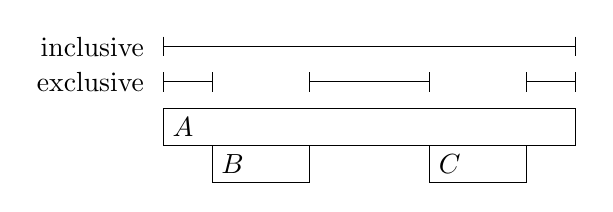
\begin{tikzpicture}[]

\node [draw     , rectangle, text width = 5cm                ] (m) {$A$};
\node [draw=none, text=white, below=-\pgflinewidth of m      ] (x) {$A$};
\node [draw     , rectangle, text width=1cm, left=0.5cm of x ] (a) {$B$};
\node [draw     , rectangle, text width=1cm, right=0.5cm of x] (b) {$C$};

\node [draw=none, rectangle, xshift= \pgflinewidth/2, yshift=0.8cm+\pgflinewidth] at (m.south west) (1) {};
\node [draw=none, rectangle, xshift= \pgflinewidth/2, yshift=0.8cm]               at (a.north west) (2) {};
\node [draw=none, rectangle, xshift=-\pgflinewidth/2, yshift=0.8cm]               at (a.north east) (3) {};
\node [draw=none, rectangle, xshift= \pgflinewidth/2, yshift=0.8cm]               at (b.north west) (4) {};
\node [draw=none, rectangle, xshift=-\pgflinewidth/2, yshift=0.8cm]               at (b.north east) (5) {};
\node [draw=none, rectangle, xshift=-\pgflinewidth/2, yshift=0.8cm+\pgflinewidth] at (m.south east) (6) {};

\node [draw=none, rectangle, yshift=0.45cm] at (1) (7) {};
\node [draw=none, rectangle, yshift=0.45cm] at (6) (8) {};

\path [draw] (1.center) edge (2.center);
	\path [draw] (1.north) edge (1.south);
	\path [draw] (2.north) edge (2.south);
\path [draw] (3.center) edge (4.center);
	\path [draw] (3.north) edge (3.south);
	\path [draw] (4.north) edge (4.south);
\path [draw] (5.center) edge (6.center);
	\path [draw] (5.north) edge (5.south);
	\path [draw] (6.north) edge (6.south);
\path [draw] (7.center) edge (8.center);
	\path [draw] (7.north) edge (7.south);
	\path [draw] (8.north) edge (8.south);

\node [draw=none, left=0cm of 7, anchor=east] () {inclusive};
\node [draw=none, left=0cm of 1, anchor=east] () {exclusive};

\end{tikzpicture}


	\caption{Exclusive and inclusive time of function $A$. It has two subroutines: $B$ and $C$.}
	\label{fig:exclusive-inclusive-execution-time}
\end{figure}

Software performance analysis can roughly be put into two categories---\emph{profiling} and \emph{tracing}.
In tracing, information is exhaustively gathered, whereas profiling measures in intervals.

Profilers present a condensed view of a program's execution.
They accumulate values on a per-function- or per-line-of-source-code-basis.
The latter technique is called call path profiling~\cite{hall92}.
Profiles are typically presented as tables (e.g. Table~\ref{tab:gprof}) or bar charts.
\begin{table}[tbh]
	\centering
	\caption{Output of a profiler for an example \cpp~program run}
	\vspace{0.2cm}
	\begin{tabular}{r r | l}
		\multicolumn{1}{c}{\textbf{Time (\%)}} &
		\multicolumn{1}{c|}{\textbf{Seconds}} &
		\multicolumn{1}{c}{\textbf{Function name}} \\

		\hline

		5.44 & 1.21 & \texttt{QListData::isEmpty} \\
		2.96 & 0.66 & \texttt{QHash::findNode} \\
		2.67 & 0.60 & \texttt{QList::last} \\
		2.52 & 0.56 & \texttt{QList::isEmpty} \\
		2.04 & 0.46 & \texttt{QList::end} \\
		1.71 & 0.38 & \texttt{handleEnter} \\
		1.44 & 0.32 & \texttt{FunctionCall::FunctionCall} \\
		0.58 & 0.13 & \texttt{QHash::find} \\
		0.56 & 0.13 & \texttt{QHashNode::same\_key} \\
		0.34 & 0.08 & \texttt{std::forward} \\
	\end{tabular}
	\label{tab:gprof}
\end{table}

To obtain the required information for generating a profile, the underlying framework uses sampling.
\emph{Sampling} probes the running program in intervals and stores information like the active function call stack, the currently executed CPU\footnote{short for central processing unit} instruction and auxiliary metrics.
The intervals are usually one or ten milliseconds long.
Due to this, one cannot generally guarantee correctness of derived statistics.
An error estimate as a function of event rate and sampling rate can be given.
Profiles are typically small in file size and the generated runtime overhead is low.
By modifying the sampling rate one can adjust the incurred overhead.

There exists a multitude of profilers differing in focus and functionality.
Most prominent is GNU~gprof~\cite{graham82}, which supports profiling single-threaded applications.
The Google Performance Tools~\cite{googleperftools} include a profiler that is similar to gprof, but supports multithreading.
Another similar tool is Callgrind~\cite{callgrind} along with the visualisation program KCachegrind~\cite{weidendorfer08}.
These three profilers have in common that they do not directly support multi-process programming.
An application is assumed to consist of exactly one process.

Much of scientific computing takes places on clusters of computers.
Leveraging their potential requires multi-process programs, which in turn need performance tuning.
Three tools that support this kind of application are Allinea~MAP~\cite{allineamap}, HPCToolkit~\cite{adhianto10} and Open|Speedshop~\cite{schulz08}.

A more detailed way of measuring software performance is tracing.
Unlike profiling, every function call is recorded and, depending on the actual implementation, for each of them all measurements are taken.
As a result of the potentially large amount of recorded information, trace visualisers typically employ interactive presentation techniques.
Figure~\ref{fig:trace-example-screenshot} shows one such visualisation, in which users can zoom in and out, choose different views and filter events to investigate their application's runtime behaviour.
\begin{figure}[tbh]
	% traces/sweep3d
	\centering
	\includegraphics[width=13.08cm]{trace-example-screenshot}
	\caption{Example trace visualisation showing (from top to bottom) a summary view of active functions over the course of the program run, a timeline showing which function is active on different processes/threads, and the call stack over time of process 0. Black lines between processes indicate communication.}
	\label{fig:trace-example-screenshot}
\end{figure}
To be able to record every entry into and exit from a function, tracing environments \emph{instrument} an application.
The added monitoring code writes the measurement results along with a timestamp into a log file.
This file is called the \emph{trace file}.
The amount of application-unrelated work incurred by tracing depends mainly on the rate of recorded events.
Function enter and leave events occur at a rapid pace.
Therefore, tracing overhead is typically very large compared to profiling.
There exist various ways to reduce this overhead including tracing only a subset of functions e.g. only certain API\footnote{short for application programming interface} calls, recording only a limited number of calls to a function, and tracing only during an interval instead of the whole program's runtime.

As a representative of tracing software, the Vampir~Tool-Set~\cite{knuepfer08b}, developed at the Technische Universit\"at Dresden, is widely deployed on high performance computers.
It consists of the open-source trace recording infrastructure VampirTrace~\cite{vampirtrace}, the open-source trace file format OTF~\cite{knuepfer06} and the commercially available visualiser Vampir.
Figure~\ref{fig:vampir-example-screenshot} shows Vampir's tiled user interface.
\begin{figure}[tbh]
	% traces/gromacs-mpmd-jens-doleschal-1
	\centering
	\includegraphics[width=13.08cm]{vampir-example-screenshot}
	\caption{Example screenshot of Vampir visualising a trace. The left display shows which functions are active on different processes and threads during program execution. The top-right display depicts a profile. The bottom-right indicates how many messages a process exchanges with which other processes.}
	\label{fig:vampir-example-screenshot}
\end{figure}
Each so-called \emph{display} presents a different view on the recorded information.
The topmost display is the \emph{Zoom Toolbar}, which provides simple, intuitive navigation.
It presents a summarised view of the program activity over time.
Colours encode different functions or groups of functions.
In this example, inter-process communication functions are red and OpenMP~\cite{openmp} (multithreading-related) functions are light blue.
The \emph{Master Timeline} is located on the left.
Processes, threads and graphics accelerator streams are arranged vertically.
For each of these and each point in time, the currently active function is coded in colour.
Arrows and black lines depict inter-process communication.
The user can zoom in horizontally and vertically to restrict the shown time interval and processes.
At the top-right, a flat profile is depicted as a bar chart.
In this figure, it shows function groups instead of functions.
The \emph{Communication Matrix View} can be found at the bottom-right.
It visualises different metrics related to inter-process communication for each pair of partners.
Here, the number of messages, coded in colour, between processes is depicted.

Another tracing tool chain is Scalasca~\cite{geimer10}, which is developed at the Forschungszentrum J\"ulich.
Aside from recording traces, it has built-in wait state detection and comes with the visualisation program Cube~\cite{song04}.
The jointly developed successor of, both, VampirTrace and Scalasca is the performance measurement infrastructure Score-P~\cite{scorep10}.
Along with it comes the new file format OTF~2.

Similarly to Vampir, the Intel Trace Analyzer~\cite{ita} provides trace visualisation, but with a more limited set of features.
Another trace viewer is Paraver~\cite{pillet95}.
It is more customisable than others and comes with a flexible file format that has no pre-defined semantics.
Everything recorded can be combined and visualised in various ways.

Tau~\cite{shende06} is yet another tracing tool, and offers the full bandwidth of recording, analysis and visualisation.

Most of the mentioned tools use a hybrid approach between profiling and tracing.
API calls of special interest are traced, whereas the rest of the program is recorded via sampling.
Some tracing environments also support sampling.
Most tracing tools can derive a profile from a trace file.
Because of this, a clear distinction cannot be drawn.

The ultimate goal of performance analysis is to help the application developer find performance problems in his code.
Programs are becoming increasingly parallel because of rising core counts and the use of specialised accelerators like GPGPUs\footnote{General-purpose computing graphics processing units}, FPGAs\footnote{Field-programmable gate array} and the Intel XEON Phi Coprocessor~\cite{xeonphi}.
The resulting challenges for performance analysis tools can be divided into two categories---data structures and algorithms on the one hand, and visualisation on the other.
Tools developers need to design for limited main memory size and need to achieve scalability with respect to the degree of parallelism used in the to-be-analysed application, the degree of parallelism used for analysis and the size of the trace file.
Visualisation tools need to cope with a limited number of pixels on the screen and achieve scalability with respect to the degree of parallelism employed in applications.
Cases where plain display of performance data is problematic already exist.
Figure~\ref{fig:more-processes-than-pixels-vertically-vampir-screenshot} is a screenshot of a visualisation for 16,384 processes.
\begin{figure}[tb]
	% fd4-16384p-bluegenep
	\centering
	\includegraphics[width=13.08cm]{more-processes-than-pixels-vertically-vampir-screenshot}
	\caption{Visualisation where the number of processes exceeds the amount of horizontal and vertical pixels.}
	\label{fig:more-processes-than-pixels-vertically-vampir-screenshot}
\end{figure}
Screens do not have as many pixels horizontally nor vertically.
In the near future, there will exist applications with millions of concurrent threads of execution.

Performance analysis tools mostly present raw data.
Profiles accumulate over all threads and each function call.
Trace visualisers present timelines, profiles and communication matrices.
Most tools lack the ability to compare measurements between threads or different function calls.
Surveying the use of comparative techniques in performance analysis will be the topic of the next section.

%%%%%%%%%%%%%%%%%%%%%%%%%%%%%%%%%%%%%%%
\section{Comparative Performance Analysis}
\label{sec:background-comparative}
Being able to compare performance measurements helps in a number of ways.
Developers can improve the visual scalability of existing tools by, for example, collapsing similar processes and just displaying one representative.
This saves precious screen space.
On the other hand new visualisations, which display comparison information, can be implemented.
Showing timing differences between processes helps exposing load imbalance problems in parallel applications.
In-depth comparison of timing before and after an optimisation pass aids developers understanding their programs.
To analyse hardware differences, fine-grained comparison of program runs between platforms or perhaps different compilers seems worthwhile.

Open|SpeedShop~\cite{schulz08} calculates differences between profiles.
Similarly, eGprof~\cite{schulz07} compares two GNU~gprof profiles, and can also show differences between call trees.
A \emph{call tree} is a tree representing all encountered function call stack configurations.
Aside from analysing differences between profiles, Cube can also combine performance information of multiple program runs into new theoretical ones that use untried program configurations.
The goal here is to reduce the number of test runs necessary to analyse a large number of configurations of a program.

Vampir can display an arbitrary number of traces side-by-side to simplify visual inspection of differences.
Intel Trace Analyzer is able to do the same, but additionally computes differences and speedup based on profiles.

By evaluating differences between specific performance metrics over time, Mohror and Karavanic~\cite{mohror09} are able to detect segments of a program run, like loops and I/O phases.
This information is then used to only store one representative segment and thus reduce trace file size and analysis overhead.
Casas et al.~\cite{casas10} suggest to construct discrete signals from sampled metrics, e.g. the signal of active number of compute processes over time.
Wavelet and correlation analysis, known from the field of signal processing, is then performed on these signals to differentiate phases of a program run and speed up analysis by focussing on representative regions.

Kn\"upfer~\cite{knuepfer07,knuepfer08a} proposes the \emph{Compressed Complete Call Graph}.
This in-memory data structure behaves like a trace, but internally uses a lossy compression scheme that relies on similarities in function call structure and relative timing.
The technique is also used to highlight repeating function call patterns in a prototype visualisation.
Ratn et al.~\cite{ratn08} employ comparison techniques to achieve lossless compression of communication traces.

Weber et al.~\cite{weber12, weber13} apply sequence alignment algorithms to the function call stack over time to detect differences between processes.
Based on this, similarity metrics and a prototype visualisation are devised.
Juckeland and Reiniger~\cite{juckeland12, reiniger13} introduced the so-called \emph{Parallel Program Flow Graph}, which unifies the sequence of active functions over time of multiple processes.
Based on this, they propose a visualisation scheme that saves screen space compared to current timeline views.
To compare the function call sequences Kn\"upfer's and Weber's methods are used.

This section suggests that differential profile analysis is well researched, but implementations exist almost exclusively in academia.
Differential trace analysis and visualisation is young and only prototype implementations exist.

As a special type of comparative technique, the next section gives an overview about the use of clustering in performance analysis and motivates the development of specialised, more scalable clustering schemes.

%%%%%%%%%%%%%%%%%%%%%%%%%%%%%%%%%%%%%%%
\section{Clustering}
\label{sec:background-clustering}
One goal of comparative analysis is to group similar processes into clusters.
Jain~\cite{jain10} gives an excellent overview about currently employed techniques.
Common clustering algorithms, for example $k$-means~\cite{forgy65, lloyd82, macqueen67, steinhaus56} and DBSCAN~\cite{ester96}, take as input $n$ points in a $d$-dimensional space or a matrix containing the similarity of each pair of points plus the goal number of clusters $k$.
The output is a set of disjoint sets, called clusters, each of which contains points considered similar.
Here, most of the time points are processes and the dimensions are performance metrics.

Juckeland and Reiniger's method, mentioned in the previous section, provides a clustering in the sense that equal functions are merged and processes are, thus, clustered.

% http://www.bsc.es/computer-sciences/performance-tools/clustering
Gonzales et al.~\cite{gonzalez09a} describe a tool that characterises computation phases, the time between inter-process communication, using two metrics---instructions per second and completed instructions.
It then clusters these periods, using the two metrics as dimensions, applying the DBSCAN algorithm.
The result is a classification of phases, that differ in instructions per second executed in a certain amount of time.
These periods are coloured differently to improve visualisation.
In a follow-up paper~\cite{gonzalez09b} the authors employ alignment techniques to evaluate the quality of their structure detection approach for multiple cases.

To reduce the file size of so-called \emph{effort traces}, Gamblin et al.~\cite{gamblin10} introduced a parallel version of the $k$-medoids~\cite{kaufman87} clustering scheme.
The method is used to detect similar processes of which only one representative is stored.
It is possible to reconstruct the complete effort trace afterwards.

Vampir's \emph{Process Summary} display, proposed by Brunst~\cite{brunst07}, uses clustering to show a condensed view of the profiles of all individual processes.
Figure~\ref{fig:clustering-in-vampir} shows this display, along with the traditional, accumulated profile for context.
To determine the clusters, $k$-means is used.
The dimensions are the ten functions with the largest accumulated exclusive execution time.
Each point is a process with its accumulated exclusive time for each of these functions as values.
Users can choose the goal number of clusters, which defaults to the number of bars that fit into the available drawing height.
The result is a clustering where processes sharing similar profiles are grouped together.
Each cluster is represented as a stacked bar chart.
On the left, next to the bars, the number of processes in the cluster and the positions of them among all processes is depicted.
In each bar there is a staircase representation marking minimum, average and maximum of the accumulated exclusive execution time of this function among the processes in the cluster.
\begin{figure}[tb]
	% traces/gromacs-mpmd-jens-doleschal-1
	\centering
	\includegraphics[width=13.08cm]{clustering-in-vampir}
	\caption{Vampir's Process Summary uses clustering to indicate similarities and differences between profiles of all individual processes. The right shows the traditional profile, which accumulates values for all processes.}
	\label{fig:clustering-in-vampir}
\end{figure}

Common clustering algorithms, including $k$-means and DBSCAN, take at least $\mathcal{O}(n^2)$ steps to cluster $n$ processes.
Calculating the similarity matrix, in preparation for clustering, requires an all-to-all comparison and, therefore, takes at least $\mathcal{O}(n^2)$ steps, too.
For 50,000 processes, regardless of dimensionality and similarity measure, the number of steps is already very large.
Common clustering algorithms, also, make assumptions about the data.
For example, $k$-means requires clusters to be shaped roughly spherically.
Using DBSCAN is problematic when different clusters differ in density.
Another downside is that most algorithms need to be provided with a goal number of clusters, which leads to unnatural clusters.
One suggested remedy is to apply clustering repeatedly and evaluate and compare the quality of the results.
To obtain a natural clustering of processes in less than $\mathcal{O}(n^2)$ steps requires a different approach.

The following chapter introduces a set of techniques to efficiently cluster processes.
The clustering, which depends only on profile information, is used to characterise traces of individual process.
This characterisation can subsequently be used in a variety of ways including choosing representative processes and choosing similar processes for in-depth performance comparison.

%%%%%%%%%%%%%%%%%%%%%%%%%%%%%%%%%%%%%%%%%%%%%%%%%%%%%%%%%%%%%%%%%%%%%%%%%%%%%%
\chapter{New Methods for~Comparative~Performance~Analysis}
\label{sec:new}
After providing some notation and general definitions, a novel structural similarity measure is proposed.
The next section introduces an efficient mechanism to store the measure for all processes.
Completing the picture, computational complexity properties of the introduced techniques are analysed.
In the last section, a variation of the approach is used to detect a special case of dissimilarity.

%%%%%%%%%%%%%%%%%%%
\section{Preliminaries}
\label{sec:new-preliminaries}
This section enumerates conventions that are used throughout the thesis.
\begin{itemize}
	\item Numerous terms exist to describe what is essentially a thread of execution.
		Individual terms vary in technical details and in which context they are used.
		Examples include process, thread and CUDA stream~\cite{cuda}.
		To avoid the lengthy \emph{thread of execution} and the ambiguous \emph{thread}, throughout this thesis \emph{process} is used to describe all of them.\vspace{-0.5ex}
		Usually, the difference between individual terms does not matter, if so, it is highlighted.
	\item In general, everything in particular sets, relations, domains and co-domains of functions are assumed to be finite.
		This does not restrict the applicability of what follows.
		It merely removes some of the intricacies of subsequent definitions and assertions.\vspace{-0.5ex}
	\item $\mathcal{P}$ denotes the set of all processes.
		Individual processes are labelled $P, P_1, P_2, P_3, \ldots$ or have actual names like \texttt{process~1} and \texttt{thread~3}.
		Similarly, $\mathcal{F}$ denotes the set of all program functions.
		Individual functions are labelled $F, F_1, F_2, F_3, \ldots$ or $A, B, C, D, \ldots$ or have actual names like \texttt{main} and \texttt{fopen}.\vspace{-0.5ex}
	\item Let $S$ be a set. $2^S$ denotes the set of all subsets of S, also called the power set of S.
\end{itemize}

%%%%%%%%%%%%%%%%%%%
\section{A Structural Similarity Measure}
\label{sec:new-structural}
A \emph{similarity measure} can be defined as a function $s : \mathcal{P} \times\nobreak \mathcal{P} \to \mathopen[ 0, 1 \mathclose]$ which satisfies the following conditions:
\begin{equation*}
	\begin{aligned}
		& \text{for all}~P_1, P_2 \in \mathcal{P} : 0 \le s(P_1, P_2) \le 1 \\
		& \text{for all}~P_1, P_2 \in \mathcal{P} : s(P_1, P_2) = s(P_2, P_1) \\
		& \text{for all}~P \in \mathcal{P} : s(P, P) = 1
	\end{aligned}
\end{equation*}
That means, it maps two processes to a real number between 0 and 1, is symmetric and yields 1 if both arguments coincide.
The lower the number, the less similar two processes are with regard to the chosen measure.

One approach to capture a process's structure is to record the functions it invokes.
The mapping \emph{functions} assigns each process the set of functions it calls during a program run.
Formally:
\begin{equation*}
	\begin{aligned}
		& \text{functions} : \mathcal{P} \to 2^\mathcal{F} \\
		& \text{functions}(P) := \{ F \in \mathcal{F} \mid F~\text{is called at least once on}~P \}
	\end{aligned}
\end{equation*}

Processes that have many functions in common are likely similar.
Therefore, using the Jaccard index~\cite{jaccard01}, structural similarity of two processes can now be expressed as the number of functions they have in common divided by the number of functions either process calls. More formally:
\begin{equation*}
	\text{functionsimilarity}(P_1, P_2) := \frac{ \mid \text{functions}(P_1) \cap \text{functions}(P_2) \mid }{ \mid \text{functions}(P_1) \cup \text{functions}(P_2) \mid }
\end{equation*}
If both sets are empty, the result is defined to be 1.
As required for being a similarity measure, the result is always between 0 and 1.
The measure is also symmetric, since union and intersection of sets is commutative.
Similarly, comparing a process to itself yields 1, because union and intersection of sets are idempotent.

Figure~\ref{fig:example-call-tree} depicts two example call trees that serve as an illustration for the proposed measure.
Call trees represent all encountered function call stack configurations of a program run.
Here, the function sets are identical, since both processes call the same functions, i.e.:
\begin{equation*}
	\begin{aligned}
		\mathrm{functions}(\texttt{process 1}) & = \mathrm{functions}(\texttt{process 2}) \\
		                                       & = \{ \texttt{main},~ \texttt{MPI\_Init},~ \texttt{fopen},~ \texttt{fclose} \}
	\end{aligned}
\end{equation*}
Therefore, similarity according to function similarity is 1.
\begin{equation*}
	\text{functionsimilarity}(\texttt{process 1}, \texttt{process 2}) = 1
\end{equation*}
A more complex example will be provided below.
Before that, a second structural similarity measure is introduced.
\begin{figure}[tb]
	\centering
	\input{tikz/example-call-tree}
	\caption{Call trees for two processes of an example program run}
	\label{fig:example-call-tree}
\end{figure}

Considering only called functions is limited in expressiveness.
What a program function computes also depends on supplied arguments, global state and external influences.
Incorporating these factors is hard due to the sheer size of argument domains, number of different states and limited predictability.
Therefore, a simpler variant providing some context to function invocations is proposed.
It uses function pairs instead of single functions.
Such a pair consist of a function which calls a function.
Formally:
\begin{equation*}
	\begin{aligned}
		& \text{functionpairs} : \mathcal{P} \to 2^{\mathcal{F} \times \mathcal{F}} \\
		& \text{functionpairs}(P) := \{ (F_1, F_2) \in \mathcal{F} \times \mathcal{F} \mid F_1~\text{calls}~F_2~\text{at least once on}~P \}
	\end{aligned}
\end{equation*}
The previously introduced principles still hold for pairs, thus \emph{function pair similarity} is defined as follows:
\begin{equation*}
	\text{functionpairsimilarity}(P_1, P_2) := \frac{ \mid \text{functionpairs}(P_1) \cap \text{functionpairs}(P_2) \mid }{ \mid \text{functionpairs}(P_1) \cup \text{functionpairs}(P_2) \mid }
\end{equation*}
To improve readability, $F_1 \rightarrow F_2$ denotes the pair $(F_1, F_2)$.

An example, using the above call trees (Figure~\ref{fig:example-call-tree}) shall illustrate the measure.
The function pair set of each process contains exactly the directed edges of the corresponding call tree, i.e.:
\begin{equation*}
	\begin{aligned}
		\text{functionpairs}(\texttt{process 1}) = \{
			& 0 \rightarrow \texttt{main},~\texttt{main} \rightarrow \texttt{MPI\_Init}, \\
			& \texttt{main} \rightarrow \texttt{fopen},~\texttt{main} \rightarrow \texttt{fclose}, \\
			& \texttt{MPI\_Init} \rightarrow \texttt{fopen},~\texttt{MPI\_Init} \rightarrow \texttt{fclose}\} \\
			\text{functionpairs}(\texttt{process 2}) = \{
			& 0 \rightarrow \texttt{main},~\texttt{main} \rightarrow \texttt{MPI\_Init}, \\
			& \texttt{MPI\_Init} \rightarrow \texttt{fopen},~\texttt{MPI\_Init} \rightarrow \texttt{fclose}\}
	\end{aligned}
\end{equation*}
Set semantics removes duplicate elements.
Incidentally, there are no duplicate pairs in this example.
Because, in principle, processes can have multiple functions on the base level, not just \texttt{main}, a virtual root function called 0 is used.
Another problem without this function, would be if the call stack had depth 1.
No pairs would then be recorded.
To obtain the function pair similarity, first the intersection and union of both function pair sets has to be computed.
\begin{equation*}
	\begin{aligned}
		\text{functionpairs}(\texttt{process 1}) \cap \text{functionpairs}(\texttt{process 2}) & = \text{functionpairs}(\texttt{process 2}) \\
		\text{functionpairs}(\texttt{process 1}) \cup \text{functionpairs}(\texttt{process 2}) & = \text{functionpairs}(\texttt{process 1})
	\end{aligned}
\end{equation*}
Next, one can take the size of the sets
\begin{equation*}
	\begin{aligned}
		\mid \text{functionpairs}(\texttt{process 1}) \cap \text{functionpairs}(\texttt{process 2}) \mid & = 4 \\
		\mid \text{functionpairs}(\texttt{process 1}) \cup \text{functionpairs}(\texttt{process 2}) \mid & = 6 \\
	\end{aligned}
\end{equation*}
and, finally, obtain the desired quotient.
\begin{equation*}
	\begin{aligned}
		& \text{functionpairsimilarity}(\texttt{process 1}, \texttt{process 2}) \\
		& \qquad = \frac{ \mid \text{functionpairs}(\texttt{process 1}) \cap \text{functionpairs}(\texttt{process 2}) \mid }{ \mid \text{functionpairs}(\texttt{process 1}) \cup \text{functionpairs}(\texttt{process 2}) \mid } \\
		& \qquad = \frac{2}{3} \approx 66.6\%
	\end{aligned}
\end{equation*}
The processes have four function pairs of a total of six in common.
Therefore, the similarity according to this measure is approximately 66.6\%.
In this work, the focus lies on function pair similarity.
For brevity and ease of presentation, the measure based on single functions is sometimes used.

One alternative to the above techniques is to compare call trees.
Andreas Kn\"upfer~\cite{knuepfer07}, introduced in Section~\ref{sec:background-comparative}, uses tree comparison to compress trace files.
Adapting the approach for call trees, the idea is as follows.
Take the call tree and unite all nodes, bottom-up, that have identical sub-trees.
Using the example from above (Figure~\ref{fig:example-call-tree}), compressing process~1's call tree yields the one depicted in Figure~\ref{fig:ccg-example-1}.
Next, process~2 can be added and then compression can be applied again.
The result is presented in Figure~\ref{fig:ccg-example-2}.
One straightforward way to measure similarity of compressed call trees is to divide the number of shared nodes by the number of all nodes.
\begin{figure}[tb]
	\centering
	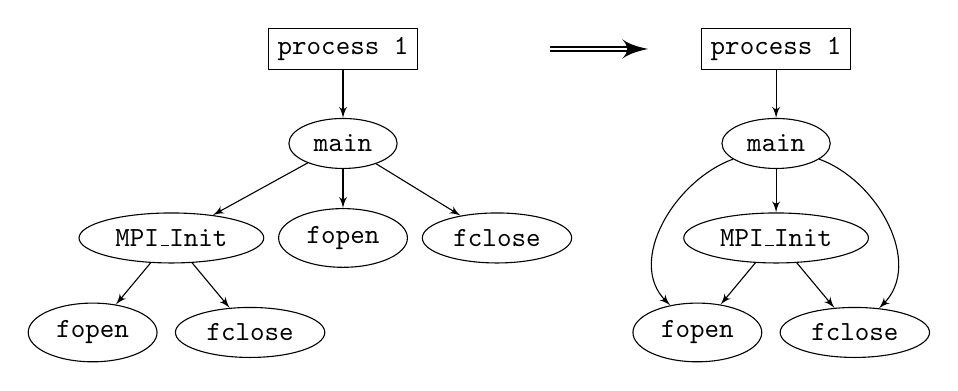
\begin{tikzpicture}[]

\node [draw     , rectangle                                         ] (p1) {\texttt{process 1}};
\node [draw     , ellipse  , below of=p1             , yshift=-0.2cm] (11) {\texttt{main}};
\node [draw     , ellipse  , below of=11             , yshift=-0.2cm] (21) {\texttt{fopen}};
\node [draw     , ellipse  , left  of=21, anchor=east               ] (31) {\texttt{MPI\_Init}};
\node [draw     , ellipse  , right of=21, anchor=west               ] (41) {\texttt{fclose}};
\node [draw=none           , below of=31             , yshift=-0.2cm] (51) {};
\node [draw     , ellipse  , left  of=51                            ] (61) {\texttt{fopen}};
\node [draw     , ellipse  , right of=51                            ] (71) {\texttt{fclose}};

\path [draw, -latex'] (p1) edge (11);

\path [draw, -latex'] (11) edge (21);
\path [draw, -latex'] (11) edge (31);
\path [draw, -latex'] (11) edge (41);

\path [draw, -latex'] (31) edge (61);
\path [draw, -latex'] (31) edge (71);


\node [draw=none, right of=p1, xshift=1.5cm   ] (m1) {};
\node [draw=none, right of=m1, xshift=0.5cm   ] (m2) {};
\path [draw, -latex', double, thick] (m1) -- (m2);


\node [draw     , rectangle, right of=m2, xshift=0.5cm ] (p2) {\texttt{process 1}};
\node [draw     , ellipse  , below of=p2, yshift=-0.2cm] (12) {\texttt{main}};
\node [draw     , ellipse  , below of=12, yshift=-0.2cm] (32) {\texttt{MPI\_Init}};
\node [draw=none           , below of=32, yshift=-0.2cm] (52) {};
\node [draw     , ellipse  , left  of=52               ] (62) {\texttt{fopen}};
\node [draw     , ellipse  , right of=52               ] (72) {\texttt{fclose}};

\path [draw, -latex'] (p2) edge (12);

\path [draw, -latex'] (12) [out=200, in=135] edge (62);
\path [draw, -latex'] (12) [out=-20, in=45 ] edge (72);

\path [draw, -latex'] (12) edge (32);
\path [draw, -latex'] (32) edge (62);
\path [draw, -latex'] (32) edge (72);

\end{tikzpicture}


	\caption{Example compressed call tree for one process}
	\label{fig:ccg-example-1}
\end{figure}
\begin{figure}[tb]
	\centering
	\begin{tikzpicture}[]

\node [draw     , rectangle, right of=m1, xshift=0.5cm  ] (p1) {\texttt{process 1}};
\node [draw     , ellipse  , below of=p1, yshift=-0.2cm ] (11) {\texttt{main}};
\node [draw     , ellipse  , below of=11, yshift=-0.2cm ] (31) {\texttt{MPI\_Init}};
\node [draw=none           , below of=31, yshift=-0.2cm ] (51) {};
\node [draw     , ellipse  , left  of=51                ] (61) {\texttt{fopen}};
\node [draw     , ellipse  , right of=51                ] (71) {\texttt{fclose}};

\path [draw, -latex'] (p1) edge (11);

\path [draw, -latex'] (11) [out=200, in=135] edge (61);
\path [draw, -latex'] (11) [out=-20, in=45 ] edge (71);

\path [draw, -latex'] (11) edge (31);
\path [draw, -latex'] (31) edge (61);
\path [draw, -latex'] (31) edge (71);


\node [draw, rectangle, right of=p1, xshift=2cm   ] (p2) {\texttt{process 2}};
\node [draw, ellipse  , below of=p2, yshift=-0.2cm] (12) {\texttt{main}};

\path [draw, -latex'] (p2) edge (12);
\path [draw, -latex'] (12) edge (31);

\end{tikzpicture}

	\caption{Example compressed call tree for two processes}
	\label{fig:ccg-example-2}
\end{figure}

Merging only absolutely equal sub-trees proved to be subpar for quantifying similarity.
Oftentimes, there are small differences in sub-trees which results in nodes not being merged.
An example, using the call trees in Figure~\ref{fig:ccg-counter-example}, illustrates this.
Processes~1 and 2 are equal to the point where function $C$ calls additionally $D$ on process~1.
No nodes would be merged, since the trees do not contain any equal sub-tree.
The resulting similarity is 0.
Using function pair similarity, instead, yields a more reasonable $\frac{3}{4}$.
Any similarity measure for compressed call trees based on the number of shared nodes has this problem.
\begin{figure}[tb]
	\centering
	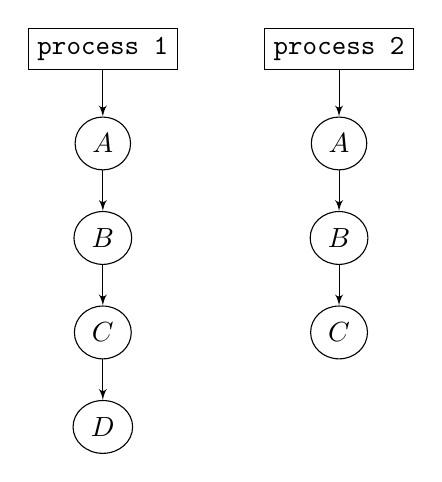
\begin{tikzpicture}[]

\node [draw, rectangle                            ] (p1) {\texttt{process 1}};
\node [draw, ellipse  , below of=p1, yshift=-0.2cm] (a1) {$A$};
\node [draw, ellipse  , below of=a1, yshift=-0.2cm] (b1) {$B$};
\node [draw, ellipse  , below of=b1, yshift=-0.2cm] (c1) {$C$};
\node [draw, ellipse  , below of=c1, yshift=-0.2cm] (d1) {$D$};

\path [draw, -latex'] (p1) edge (a1);
\path [draw, -latex'] (a1) edge (b1);
\path [draw, -latex'] (b1) edge (c1);
\path [draw, -latex'] (c1) edge (d1);

\node [draw, rectangle, right of=p1, xshift=2.0cm ] (p2) {\texttt{process 2}};
\node [draw, ellipse  , below of=p2, yshift=-0.2cm] (a2) {$A$};
\node [draw, ellipse  , below of=a2, yshift=-0.2cm] (b2) {$B$};
\node [draw, ellipse  , below of=b2, yshift=-0.2cm] (c2) {$C$};

\path [draw, -latex'] (p2) edge (a2);
\path [draw, -latex'] (a2) edge (b2);
\path [draw, -latex'] (b2) edge (c2);

\end{tikzpicture}

	\caption{Example Call tree that would not be merged using sub-tree matching}
	\label{fig:ccg-counter-example}
\end{figure}

If call trees are equal, function pair similarity as well yields 1, since having equal sub-trees implies identical function pair sets.
Depending on how recursion is dealt with, function pair similarity of two processes is almost always higher than call tree similarity (number of shared nodes divided by number of all nodes).
% counter example, because of which there is 'almost':
%
% 0     1*
% |\   /|
% | \ / |
% A* B  C*
%
% according to call tree = 1/5
% according to func pair = 1/6

Function pair similarity is influenced by the functions a processes calls and where they are called from.
Inlining functions, for example, changes the similarity value.
The number of calls and their timing does not influence the outcome of comparing two processes.
It, therefore, also ignores how many iterations of a loop are done.
If calls are reordered inside a function, similarity does not change.
Recursion is problematic for some analysis tools and workflows, since the resulting call trees and stacks can get very deep and, compared to the structure of the source code, falsely represent program structure.
Function pair similarity handles this gracefully, because if $F$ is recursive, only the pair $F \rightarrow F$ is added.
Recursion depth is ignored.

Concluding the previous observations, function pair similarity evaluates structure, regardless of timing, iteration counts and recursion depth.
Processes with 100\% similarity form groups.
The number of such groups is supposed to be stable with increasing process counts, and thus should provide a scalable grouping.
Statically compiled source code is expected to not call different functions when problem size or process numbers vary~\cite{allineaddt, arnold07, johnson91}.
Chapter~\ref{sec:evaluation} analyses whether this expectation holds in practice.

Mind that applying the measure is not restricted to processes of one program run.
It can also be employed to compare multiple runs and even different programs.
Similar processes can, therefore, be identified across runs in preparation for in-depth comparative performance analysis.

To be useful for large numbers of processes, calculating the measure for all pairs of processes in sub-quadratic time is key.
In order to achieve this, per-process information, required to compute the measure, needs to be stored in a manner that reduces the data so that subsequent querying for similarity values is quick.
Alternatively, one can store everything in a straightforward manner and devise a sub-quadratic querying algorithm.
The next section elaborates how efficient similarity storage and computation is achieved.

%%%%%%%%%%%%%%%%%%%
\vspace{1.5ex}
\section{Efficient Storage and Calculation of Set-Based Metrics}
\label{sec:new-storage}
\vspace{1.5ex}
To calculate similarity, the set of function pairs for each process is needed.
Imagine straightforwardly storing all processes and set elements in a two-dimensional matrix.
The matrix elements are crosses signalling whether or not an element belongs to the process.
Further, suppose there are 1,000,000 processes with up to 1,000 set elements, and elements are identified using a 32-bit value.
Storing the whole table would then take roughly four gibibytes\footnote{$1,000,000 \times 1,000 \times 4 ~\text{bytes} = 4,000,000 ~\text{bytes}$} of storage space.
Using bit vectors, one could lower the storage need.
But this increases handling complexity and does not improve scalability.
Even requiring 100 mebibytes is still large considering the technique is used to just classify processes in preparation for deeper analysis.
Thus, the primary goal was to find a way to store all set elements and processes with few or no duplicates.

\vspace{1.0ex}
The \emph{concept lattice}, known from the field of \emph{formal concept analysis}~\cite{ganter99} emerged as a suitable data structure.
A concept lattice is a type of \emph{order}.
A \emph{total order} $R \subseteq X \times X$ on a set $X$, for example, is a binary relation that is transitive, antisymmetric and total.
Formally:
\begin{equation*}
	\begin{aligned}
		& \text{for all}~a, b, c \in X & :~ & \text{if}~(a, b) \in R~\text{and}~(b, c) \in R~\text{then}~(a,c) \in R~ & \text{(transitivity)} \\
		& \text{for all}~a, b \in X    & :~ & \text{if}~(a, b) \in R~\text{and}~(b, a) \in R~\text{then}~a = b~ & \text{(antisymmetry)} \\
		& \text{for all}~a, b \in X    & :~ & (a, b) \in R~\text{or}~(b, a) \in R~ & \text{(totality)}
	\end{aligned}
\end{equation*}
An example is the natural numbers ordered by $\le$ (Figure~\ref{fig:total-order-example}).
Removing the need for totality yields the partial order.
A \emph{partial order} $R \subseteq X \times X$ on a set $X$ is a binary relation that is transitive, antisymmetric and reflexive.
Reflexivity means each element in $X$ is related to itself.
Formally:
\vspace{2.0ex}
\begin{equation*}
	\text{for all}~a \in X: ~(a, a) \in R
\end{equation*}
An example of such an order is the natural numbers ordered by divisibility (Figure~\ref{fig:partial-order-example}).
\begin{figure}[tb]
	\centering
	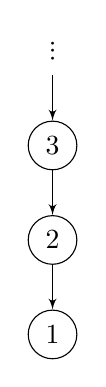
\begin{tikzpicture}[]

\node [draw=none, circle,                          ] (a) {\rotatebox{90}{...}};
\node [draw     , circle, below of=a, yshift=-0.2cm] (3) {3};
\node [draw     , circle, below of=3, yshift=-0.2cm] (2) {2};
\node [draw     , circle, below of=2, yshift=-0.2cm] (1) {1};

\path [draw, -latex'] (a) edge (3);
\path [draw, -latex'] (3) edge (2);
\path [draw, -latex'] (2) edge (1);

\end{tikzpicture}


	\caption{Example totally ordered set: $(\mathbb{N}, \le)$}
	\label{fig:total-order-example}
\end{figure}
\begin{figure}[tb]
	\centering
	\begin{tikzpicture}[]

\node [draw     , circle                                                ] (6) {6};

\node [draw     , circle, below right of=a, xshift=0.2cm , yshift=-0.2cm] (3) {3};
\node [draw     , circle, below left  of=6, xshift=-0.2cm, yshift=-0.2cm] (2) {2};
\node [draw     , circle, below right of=2, xshift=0.2cm , yshift=-0.2cm] (1) {1};

\node [draw=none, circle, above left  of=2, xshift=-0.2cm, yshift=0.2cm ] (a) {\rotatebox{135}{...}};
\node [draw=none, circle,       left  of=2                              ] (b) {...};
\node [draw=none, circle, above left  of=6, xshift=-0.2cm, yshift=0.2cm ] (c) {\rotatebox{135}{...}};
\node [draw=none, circle, above right of=6, xshift=0.2cm , yshift=0.2cm ] (d) {\rotatebox{45}{...}};
\node [draw=none, circle, above right of=3, xshift=0.2cm , yshift=0.2cm ] (e) {\rotatebox{45}{...}};
\node [draw=none, circle,       right of=3                              ] (f) {...};

\path [draw, -latex'] (a) edge (2);
\path [draw, -latex'] (c) edge (6);
\path [draw, -latex'] (d) edge (6);
\path [draw, -latex'] (e) edge (3);
\path [draw, -latex'] (6) edge (3);
\path [draw, -latex'] (6) edge (2);
\path [draw, -latex'] (3) edge (1);
\path [draw, -latex'] (2) edge (1);

\end{tikzpicture}

	\caption{Example partially ordered set: $(\mathbb{N}, \mid)$}
	\label{fig:partial-order-example}
\end{figure}
\vspace{1.0ex}

Another kind of order is the bounded lattice.
A \emph{bounded lattice} $R$ on a set $X$ is a finite partial order where for each pair of elements in $X$ there exists a unique least upper bound $\vee$ (also called supremum or join) and a unique greatest lower bound $\wedge$ (also called infimum or meet).
A supremum $s$ of two elements $a, b \in X$ is an element which satisfies the following:
\begin{equation*}
	\begin{aligned}
		& (a, s) \in R ~\text{and}~ (b, s) \in R \\
		& \text{for all}~ x \in X: ~\text{if}~ (a, x) \in R ~\text{and}~ (b, x) \in R ~\text{then}~ (s, x) \in R
	\end{aligned}
\end{equation*}
It is the smallest element that is larger than both $a$ and $b$ according to $R$.
Similarly, an infimum $i$ of two elements $a, b \in X$ satisfies:
\begin{equation*}
	\begin{aligned}
		& (i, a) \in R ~\text{and}~ (i, b) \in R \\
		& \text{for all}~ x \in X: ~\text{if}~ (x, a) \in R ~\text{and}~ (x, b) \in R ~\text{then}~ (x, i) \in R
	\end{aligned}
\end{equation*}
These properties imply that there is an absolute largest element and an absolute smallest one.
An example is the set $\{ A, B, C \}$ ordered by $\subseteq$ with the join operation being the set union and the meet being set intersection (Figure~\ref{fig:bounded-lattice-example}).
\begin{figure}[tb]
	\centering
	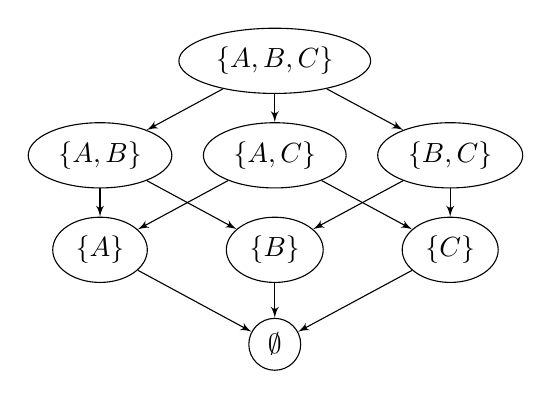
\begin{tikzpicture}[]

\node [draw, ellipse                                          ] (abc) {$\{A, B, C\}$};
\node [draw, ellipse, below of=abc             , yshift=-0.2cm] (ac)  {$\{A, C\}$};
\node [draw, ellipse, left  of=ac , anchor=east, xshift=-0.3cm] (ab)  {$\{A, B\}$};
\node [draw, ellipse, right of=ac , anchor=west, xshift=0.3cm ] (bc)  {$\{B, C\}$};
\node [draw, ellipse, below of=ac              , yshift=-0.2cm] (b)   {$\{B\}$};
\node [draw, ellipse, below of=ab              , yshift=-0.2cm] (a)   {$\{A\}$};
\node [draw, ellipse, below of=bc              , yshift=-0.2cm] (c)   {$\{C\}$};
\node [draw, circle , below of=b               , yshift=-0.2cm] (0)   {$\emptyset$};

\path [draw, -latex'] (abc) edge (ab);
\path [draw, -latex'] (abc) edge (bc);
\path [draw, -latex'] (abc) edge (ac);
\path [draw, -latex'] (ab)  edge (a);
\path [draw, -latex'] (ab)  edge (b);
\path [draw, -latex'] (bc)  edge (b);
\path [draw, -latex'] (bc)  edge (c);
\path [draw, -latex'] (ac)  edge (a);
\path [draw, -latex'] (ac)  edge (c);
\path [draw, -latex'] (a)   edge (0);
\path [draw, -latex'] (b)   edge (0);
\path [draw, -latex'] (c)   edge (0);

\end{tikzpicture}

	\caption{Example bounded lattice: $(\{A, B, C\}, \cup, \cap, \emptyset, \{ A, B, C \})$}
	\label{fig:bounded-lattice-example}
\end{figure}

Extending this, a concept lattice consists of two interlocked bounded lattices.
One is the complement of the other.
Formally, a \emph{formal context}~\cite{ganter99} is a triple $(O, A, I)$ where $O$ is the set of objects, $A$ the set of attributes and $I \subseteq O \times A$ the incidence relation.
Each object has a set of attributes.
For the use case of comparing processes, the set of objects is the set of processes, and attributes are function pairs or functions.
A formal context defines a \emph{concept lattice} by specifying so-called \emph{concepts}, and a partial order on them.
A concept lattice can be represented as a graph where concepts are nodes and the order determines the edges.
In the context of this thesis, it is not important to distinguish between formal context and concept lattice.
They represent the exact same information.

An example shall illustrate this formalism.
Let $(\mathcal{P}, \mathcal{F}, \mathcal{I})$ be a formal context where
\begin{equation*}
	\begin{aligned}
		\mathcal{P} & = \{P_1, P_2, P_3, P_4\} \\
		\mathcal{F} & = \{A, B, C\} \\
		\mathcal{I} & = \big\{(P_1, A),~(P_2, B),~ (P_2, C),~ (P_3, A),~ (P_3, B),~ (P_3, C),~ (P_4, B),~ (P_4, C)\big\}
	\end{aligned}
\end{equation*}
holds. The incidence relation $\mathcal{I}$ can also be represented as a table (Table~\ref{tab:formal-context-example}).
$P_1$ calls just $A$. $P_2$ and $P_4$ both call $B$ and $C$. $P_3$ calls all three functions.
An algorithm then extracts the concepts and the partial order on them from the formal context.
The resulting concept lattice is depicted in Figure~\ref{fig:concept-lattice-example-redundant}.
It can be read as follows:
\begin{itemize}
	\item Process sets subsume  those that are reachable following edges downwards.\vspace{-0.5ex}
	\item Function sets subsume those that are reachable following edges upwards.\vspace{-0.5ex}
	\item The top node indicates that all processes call the empty set of functions.\vspace{-0.5ex}
	\item The bottom node signifies that only $P_3$ calls all functions, and in particular that it calls every function which $P_1$, $P_2$ and $P_4$ call.\vspace{-0.5ex}
	\item $P_1$ is different from $P_2$ and $P_4$.\vspace{-0.5ex}
	\item $P_2$ and $P_4$ call the same functions.
\end{itemize}
This graph contains redundant information.
Removing it, without changing its meaning, yields the more readable graph in Figure~\ref{fig:concept-lattice-example-not-redundant}.
It can be interpreted as follows:
\begin{itemize}
	\item No process calls a common subset of functions.\vspace{-0.5ex}
	\item $P_1$ calls $A$.\vspace{-0.5ex}
	\item $P_2$ and $P_4$ call the same functions, namely $B$ and $C$.\vspace{-0.5ex}
	\item $P_3$ subsumes all other processes and, thus, calls $A$, $B$ and $C$.
\end{itemize}
\begin{figure}[tb]
	\centering
	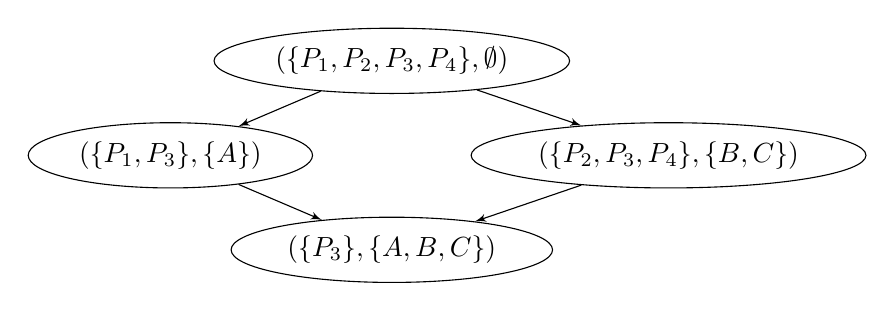
\begin{tikzpicture}[]

\node [draw     , ellipse                            ] (0)   {$(\{P_1, P_2, P_3, P_4\}, \emptyset)$};
\node [draw=none,        , below of=0 , yshift=-0.2cm] (x)   {};
\node [draw     , ellipse, left  of=x , anchor=east  ] (a)   {$(\{P_1, P_3\}, \{A\})$};
\node [draw     , ellipse, right of=x , anchor=west  ] (bc)  {$(\{P_2, P_3, P_4\}, \{B, C\})$};
\node [draw     , ellipse, below of=x , yshift=-0.2cm] (abc) {$(\{P_3\}, \{A, B, C\})$};

\path [draw, -latex'] (0)  edge (a);
\path [draw, -latex'] (0)  edge (bc);
\path [draw, -latex'] (a)  edge (abc);
\path [draw, -latex'] (bc) edge (abc);

\end{tikzpicture}

	\caption{Example concept lattice including redundant information}
	\label{fig:concept-lattice-example-redundant}
\end{figure}
\begin{figure}[tb]
	\centering
	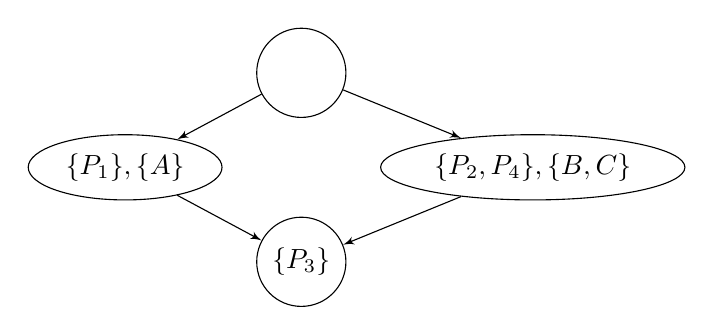
\begin{tikzpicture}[]

\node [draw     , circle , text=white                ] (0)   {$\{P_9\}$};
\node [draw=none,        , below of=0 , yshift=-0.2cm] (x)   {};
\node [draw     , ellipse, left  of=x , anchor=east  ] (a)   {$\{P_1\}, \{A\}$};
\node [draw     , ellipse, right of=x , anchor=west  ] (bc)  {$\{P_2, P_4\}, \{B, C\}$};
\node [draw     , circle , below of=x , yshift=-0.2cm] (abc) {$\{P_3\}$};

\path [draw, -latex'] (0)  edge (a);
\path [draw, -latex'] (0)  edge (bc);
\path [draw, -latex'] (a)  edge (abc);
\path [draw, -latex'] (bc) edge (abc);

\end{tikzpicture}

	\caption{Example concept lattice excluding redundant information}
	\label{fig:concept-lattice-example-not-redundant}
\end{figure}
\begin{table}[tb]
	\centering
	\caption{Example incidence relation: $\mathcal{I}$}
	\vspace{0.2cm}
	\begin{tabular}{r | c c c}
			  & $A$      & $B$      & $C$      \\
		\hline
		$P_1$ & $\times$ &          &          \\
		$P_2$ &          & $\times$ & $\times$ \\
		$P_3$ & $\times$ & $\times$ & $\times$ \\
		$P_4$ &          & $\times$ & $\times$ \\
	\end{tabular}
	\label{tab:formal-context-example}
\end{table}

A concept lattice is a directed acyclic graph of function inheritance.
Nodes inherit attributes from others that are reachable along upward-edges.
Each object and attribute is contained in the concept lattice exactly once.

Two examples shall give an intuition on concept lattices for real-world application runs.
The first one, depicted in Figure~\ref{fig:wrf-64p-concept-lattice}, is the result of a WRF~\cite{michalakes01, wrf} weather simulation run using 64 processes.
Each node contains a set of processes and function pairs.
The size of each set is given in parenthesis, followed by a few example elements.
Because internally, functions are represented by integer identifiers and to save space, numbers are used to denote functions.
In this example, every process except the first has the same function pairs.
Process~1 has 111 additional pairs.
The second example (Figure~\ref{fig:amg2006-512p-concept-lattice}) shows the concept lattice of function pairs for an AMG2006~\cite{amg} run, a differential equation solver, using 512 processes.
This lattice has 14 nodes and 21 edges, and is therefore larger and more complex than the previous lattice.
\begin{figure}[tb]
	% traces/wrf_0064cpus_fpops_l3tcm_io_mem
	\centering
	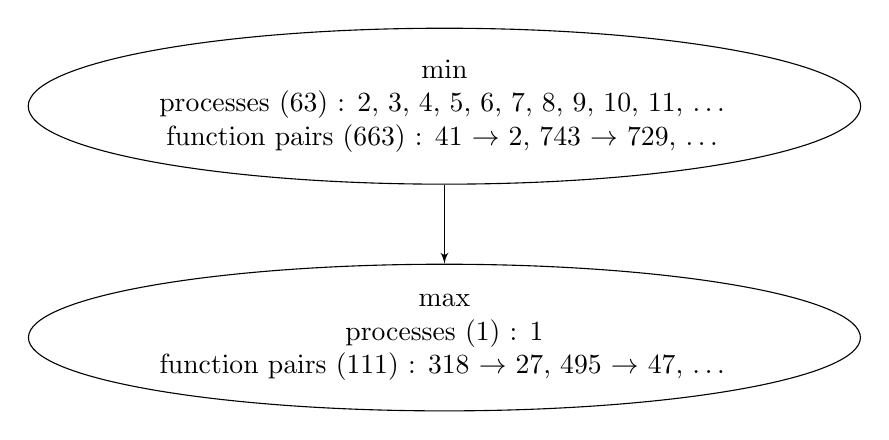
\begin{tikzpicture}[]

\node [draw, ellipse, align=center] (1) {
	min \\
	processes (63) : 2, 3, 4, 5, 6, 7, 8, 9, 10, 11, \ldots \\
	function pairs (663) : 41 $\rightarrow$ 2, 743 $\rightarrow$ 729, \ldots
};

\node [draw, ellipse, align=center, below of=1, anchor=north, yshift=-1.0cm] (2) {
	max \\
	processes (1) : 1 \\
	function pairs (111) : 318 $\rightarrow$ 27, 495 $\rightarrow$ 47, \ldots
};

\path [draw, -latex'] (1)  edge (2);

\end{tikzpicture}

	\vspace{0.5ex}
	\caption{Concept lattice of function pairs for a WRF weather simulation run utilising 64 processes}
	\label{fig:wrf-64p-concept-lattice}
	\vspace{0.5ex}
\end{figure}
\begin{figure}[tb]
	% traces/mawe-neu-2-analysis/amg2006-filt/512-proc
	\centering
	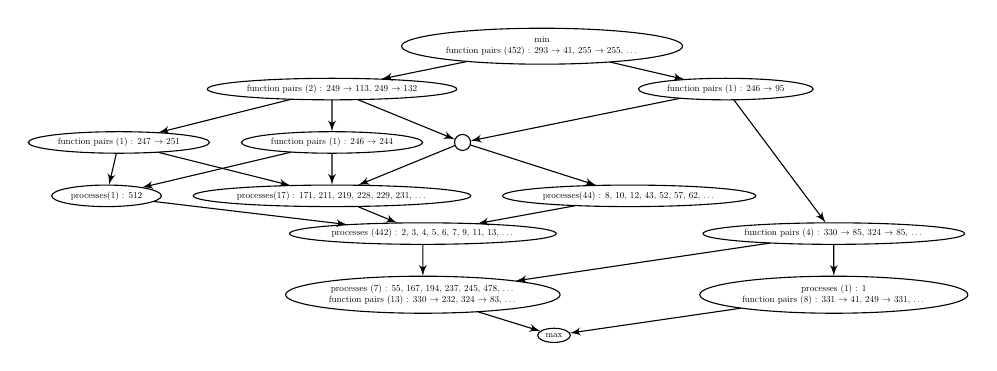
\begin{tikzpicture}[scale=0.33, every node/.style={scale=0.33}]

% top level
\node [draw, ellipse, align=center] (min) {
	min \\ function pairs (452) :  293 $\rightarrow$ 41, 255 $\rightarrow$ 255, \ldots};

% next level
\node [draw, ellipse, below left=0.4cm  of min] (blmin) {
	function pairs (2) : 249 $\rightarrow$ 113, 249 $\rightarrow$ 132};
\node [draw, ellipse, below right=0.4cm of min] (brmin) {
	function pairs (1) : 246 $\rightarrow$ 95};

\path [draw, -latex'] (min) edge (blmin);
\path [draw, -latex'] (min) edge (brmin);

% next level
\node [draw, ellipse, below=0.4cm of blmin             ] (blbmin) {
	function pairs (1) : 246 $\rightarrow$ 244};
\node [draw, ellipse, left=0.4cm  of blbmin            ] (blblmin) {
	function pairs (1) : 247 $\rightarrow$ 251};
\node [draw, circle , right=0.4cm of blbmin, text=white] (blbrmin) {0};

\path [draw, -latex'] (blmin) edge (blbmin);
\path [draw, -latex'] (blmin) edge (blblmin);
\path [draw, -latex'] (blmin) edge (blbrmin);
\path [draw, -latex'] (brmin) edge (blbrmin);

% next level
\node [draw, ellipse, below=0.4cm of blbmin ] (blbbmin) {
	processes(17) : 171, 211, 219, 228, 229, 231, \ldots};
\node [draw, ellipse, left=0.4cm  of blbbmin] (blbblmin) {
	processes(1) : 512};
\node [draw, ellipse, right=0.4cm of blbbmin] (blbbrmin) {
	processes(44) : 8, 10, 12, 43, 52, 57, 62, \ldots};

\path [draw, -latex'] (blblmin) edge (blbblmin);
\path [draw, -latex'] (blblmin) edge (blbbmin);
\path [draw, -latex'] (blbmin)  edge (blbblmin);
\path [draw, -latex'] (blbmin)  edge (blbbmin);
\path [draw, -latex'] (blbrmin) edge (blbbmin);
\path [draw, -latex'] (blbrmin) edge (blbbrmin);

% next level
\node [draw, ellipse, below left=0.4cm  of blbbrmin] (blbbrblmin) {
	processes (442) : 2, 3, 4, 5, 6, 7, 9, 11, 13, \ldots};
\node [draw, ellipse, below right=0.4cm of blbbrmin] (blbbrbrmin) {
	function pairs (4) : 330 $\rightarrow$ 85, 324 $\rightarrow$ 85, \ldots};

\path [draw, -latex'] (blbblmin) edge (blbbrblmin);
\path [draw, -latex'] (blbbmin)  edge (blbbrblmin);
\path [draw, -latex'] (blbbrmin) edge (blbbrblmin);
\path [draw, -latex'] (brmin)    edge (blbbrbrmin);

% next level
\node [draw, ellipse, align=center, below=0.4cm of blbbrblmin] (blbbrblbmin) {
	processes (7) : 55, 167, 194, 237, 245, 478, \ldots \\
	function pairs (13) : 330 $\rightarrow$ 232, 324 $\rightarrow$ 83, \ldots};
\node [draw, ellipse, align=center, below=0.4cm of blbbrbrmin] (blbbrbrbmin) {
	processes (1) : 1 \\
	function pairs (8) : 331 $\rightarrow$ 41, 249 $\rightarrow$ 331, \ldots};

\path [draw, -latex'] (blbbrblmin) edge (blbbrblbmin);
\path [draw, -latex'] (blbbrbrmin) edge (blbbrblbmin);
\path [draw, -latex'] (blbbrbrmin) edge (blbbrbrbmin);

% next level
\node [draw, ellipse, align=center, below right=0.4cm of blbbrblbmin] (max) {max};

\path [draw, -latex'] (blbbrblbmin) edge (max);
\path [draw, -latex'] (blbbrbrbmin) edge (max);

\end{tikzpicture}

	\vspace{0.5ex}
	\caption{Concept lattice of function pairs for an AMG2006 differential equation solver run utilising 512 processes}
	\label{fig:amg2006-512p-concept-lattice}
	\vspace{0.5ex}
\end{figure}

Algorithms to create concept lattices are involved and unintuitive.
Because of this and since the techniques are used without modification, elaboration on how they operate is foregone.
The interested reader is pointed towards the websites of Uta Priss~\cite{priss} and Bernhard Ganter~\cite{ganter14}, and the textbook~\cite{ganter99}.
One algorithm to create a concept lattice is, for example, \emph{Ganter's Next Closure} algorithm~\cite{ganter84, ganter99}.
It requires the complete incidence relation to be present in main memory.
As previously stated, these tables can get very large---larger than available main memory.
To avoid this, an iterative algorithm by Dean van der Merwe, Sergei Obiedkov, and Derrick Kourie~\cite{van04}---from here on called \emph{van der Merwe's algorithm}---is used.

After creating the concept lattice, the next step is to extract similarity values for each pair of processes from it.
The result is a so-called \emph{similarity matrix} which is a matrix of equivalence classes, since processes on the same lattice node yield the same values when compared to other processes.
Function similarity, which is defined as
\vspace{0.5ex}
\begin{equation*}
	\text{functionsimilarity}(P_1, P_2) := \frac{ \mid \text{functions}(P_1) \cap \text{functions}(P_2) \mid }{ \mid \text{functions}(P_1) \cup \text{functions}(P_2) \mid }
\end{equation*}
and analogously function pair similarity, can be obtained as follows.
$\text{functions}(P)$ is the union of function sets of nodes reachable along upward-edges starting at $P$'s node.
$\text{functions}(P_1) \cap \text{functions}(P_2)$ is the union of function sets of nodes reachable from both $P_1$'s and $P_2$'s node along upward-edges.
$\text{functions}(P_1) \cup \text{functions}(P_2)$ is the union of function sets of nodes reachable from either $P_1$'s or $P_2$'s node along upward-edges.
Since each function is contained in the chosen lattice representation exactly once, instead of calculating the union of sets, it suffices to take the sum of set sizes.
This yields the desired cardinality.
This approach works for functions and function pairs alike.
In fact, many more set-based measures can be handled this way.

\begin{figure}[t]
	% traces/wrf_0016cpus_hybrid_counter
	\centering
	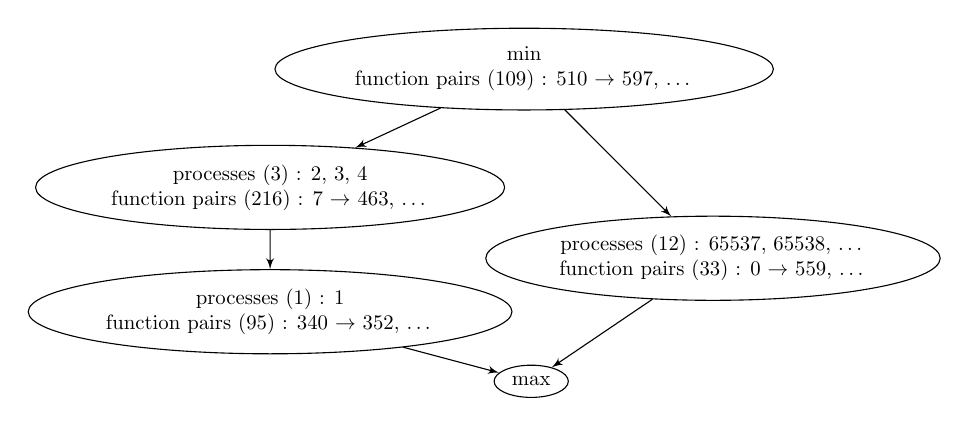
\begin{tikzpicture}[scale=0.75, every node/.style={scale=0.75}]

\node [draw, ellipse, align=center] (min) {
	min \\
	function pairs (109) : 510 $\rightarrow$ 597, \ldots};

\node [draw, ellipse, align=center, below left=0cm of min, xshift=1.5cm, yshift=-1cm] (l) {
	processes (3) : 2, 3, 4 \\
	function pairs (216) : 7 $\rightarrow$ 463, \ldots};

\node [draw, ellipse, align=center, below=0.5cm of l] (ll) {
	processes (1) : 1 \\
	function pairs (95) : 340 $\rightarrow$ 352, \ldots};

\node [draw, ellipse, align=center, right=0.5cm of l, xshift=-1cm, yshift=-1.2cm] (r) {
	processes (12) : 65537, 65538, \ldots \\
	function pairs (33) : 0 $\rightarrow$ 559, \ldots};

\node [draw, ellipse, below right=0.5cm of ll, xshift=0.6cm] (max) {max};

\path [draw, -latex'] (min) edge (l);
\path [draw, -latex'] (min) edge (r);
\path [draw, -latex'] (l)   edge (ll);
\path [draw, -latex'] (ll)  edge (max);
\path [draw, -latex'] (r)   edge (max);

\end{tikzpicture}

	\vspace{0.5ex}
	\caption{Concept lattice of function pairs for a WRF weather simulation run utilising four processes and twelve threads}
	\label{fig:wrf-hybrid-16p-concept-lattice}
	\vspace{0.5ex}
\end{figure}
An example illustrates the procedure of obtaining the similarity matrix from a lattice.
Figure~\ref{fig:wrf-hybrid-16p-concept-lattice} shows the concept lattice of a WRF run using four processes and twelve threads.
Before extracting similarities, the following explains how to read the shown lattice:
\begin{itemize}
	\item Processes have identifiers 1--4, threads have 65,537 and above.\vspace{-0.5ex}
	\item There are three groups of processes/threads: process 1, processes~2--4 and a group containing all threads.\vspace{-0.5ex}
	\item All processes and threads have 109 function pairs in common.\vspace{-0.5ex}
	\item Process~1 subsumes processes~2, 3 and 4.\vspace{-0.5ex}
	\item The twelve threads are in a group of their own and differ from the processes substantially.
\end{itemize}
To obtain the function pair similarity of processes~1 and 2, the following value needs to be calculated:
\vspace{0.5ex}
\begin{equation*}
	\frac{ \mid \text{functionpairs}(\texttt{process 1}) \cap \text{functionpairs}(\texttt{process 2}) \mid }{ \mid \text{functionpairs}(\texttt{process 1}) \cup \text{functionpairs}(\texttt{process 2}) \mid }
\end{equation*}
$\text{functionpairs}(\texttt{process 1})$ are the function pairs contained in the three nodes on the left reachable from process~1's node along upward-edges.
$\text{functionpairs}(\texttt{process 2})$ are the two nodes reachable from process~2's node along upward-edges.
The intersection of both is, therefore, the upper two nodes, whereas the union also includes the function pairs from process~1's node.
Putting it all together, function pair similarity is about 77\%. More formally:
\begin{equation*}
	\text{functionpairsimilarity}(\texttt{process 1}, \texttt{process 2}) = \frac{109 + 216}{109 + 216 + 95} \approx 77\%
\end{equation*}
Function pair similarity of processes~1 and 3, as well as 1 and 4 are the same as for processes~1 and 2.

As for comparing processes~2--4 to the threads, the intersection in the similarity formula consists of the function pairs from the uppermost node. The union contains the ones from the topmost three nodes.
Function pair similarity is therefore:
\begin{equation*}
	\text{functionpairsimilarity}(\texttt{process 2}, \texttt{thread 1}) = \frac{109}{109 + 216 + 33} \approx 30\%
\end{equation*}
The resulting similarity matrix is depicted in Table~\ref{tab:wrf-hybrid-similarity-matrix}.
Since it is symmetric and every diagonal entry is 1, it would suffice to display the three bottom-left entries.
\begin{table}[tb]
	\centering
	\caption{Similarity matrix of the WRF example run}
	\vspace{0.2cm}
	\begin{tabular}{r | r r r}
		                & Process 1 & Process 2, 3, 4 & Threads \\
		\hline
		Process 1       &    1      & 0.77            & 0.24    \\
		Process 2, 3, 4 & 0.77      &    1            & 0.30    \\
		Threads         & 0.24      & 0.30            &    1    \\
	\end{tabular}
	\label{tab:wrf-hybrid-similarity-matrix}
\end{table}

The next section discusses complexity theoretic properties and possible parallelisation of the introduced approach.

%%%%%%%%%%%%%%%%%%%
\section{Scalability Considerations}
\label{sec:new-scalability}
Obtaining the similarity of each pair of processes requires multiple steps.
First, the lattice is constructed, from which in a second step similarities are extracted.
To construct the concept lattice, for each process the set of function pairs has to be inserted using van der Merwe's algorithm.
Next, for each node in the concept lattice that has at least one process, and each other node in the concept lattice that has at least one process the graph is traversed upwards.
During this traversal, the numerator and denominator from the similarity formula for this pair of process groups are obtained.
After finishing the traversal, the fraction is calculated.

The worst-case space complexity of storing a concept lattice, as shown by Godin, Missaoui, and April~\cite{godin93}, is $\mathcal{O}(2^ap)$ where $a$ is the total number of attributes and $p$ the process count.
Therefore and according to van der Merwe et al.~\cite{van04}, the worst-case time complexity of generating the lattice and computing the similarity matrix is $\mathcal{O}(2^ap^3a)$.
The latter bound is not tight.

In practice, as mentioned in Section~\ref{sec:new-structural}, processes are expected to fall into few, i.e. a constant number of, groups.
The attribute count is constant as well, since the number of functions in a program does not increase with rising process counts or increasing problem size.
The space complexity of storing the lattice is, therefore, expected to be independent of the process and attribute count, i.e. $\mathcal{O}(1)$.
Because similarity matrix computation only depends on the number of nodes in the lattice, the most expensive part of the procedure is inserting each process's function pairs into the lattice.
Therefore, the expected time complexity of lattice creation and similarity extraction is $\mathcal{O}(p)$ with $p$ being the process count.

Being faster than linear in the number of processes is not possible when executing the steps serially, since some work has to be done for each process.
One can argue that linear time is not good enough for large process numbers.
Which is why parallelisation of the approach should be considered.
Performance analysis tools for high performance computing, especially tracing tools, heavily depend on parallelism to cope with the large amount of data and associated processing.
Algorithms to generate concept lattices in parallel already exist~\cite{hu07, liu03, njiwoua97}.
They suggest that an algorithm creating the concept lattice in expected $\mathcal{O}(\log p)$ steps can be devised.
One straightforward solution would be to first create multiple lattices in parallel.
These intermediate lattices can then be merged into a final lattice in a tree-esque or all-to-one fashion.
Merging in this case means inserting each node from the previous lattice into the new one.
Each process in a node is known to be equal according to the similarity measure and, therefore, multiple processes can be inserted in one step.
Speeding up the computation of the similarity matrix is straightforward, since each cell can independently be calculated.

The next section uses the introduced techniques with a twist to detect a special class of differences between processes.

%%%%%%%%%%%%%%%%%%%%%%%%%%%%%%%%%%%%%%%
\section{The Subsumption Measure}
\label{sec:new-subsumption}
Slightly modifying the shown techniques makes it possible to discern whether processes are dissimilar because one does additional work, i.e. performs extra function calls.
More specifically, the following cases can be distinguished from other differences:
\begin{itemize}
	\item Function calls are replaced by their implementation (\emph{inlining}).\vspace{-0.5ex}
	\item One process calls additional functions, for example when printing debug output or writing to disk.\vspace{-0.5ex}
	\item Processes have different levels of tracing detail.\vspace{-0.5ex}
	\item Threads are spawned from a process using the fork-join model.
\end{itemize}
This distinction is useful for further differential analysis, and generally automatic comparison of processes inside one and between multiple program runs.

An example (Figure~\ref{fig:subsumption-example-call-stack}) illustrates the idea.
Process~1 calls $A$, which then calls $B$.
For process~2, $A$ has been inlined and $B$ is called directly.
The resulting concept lattice is depicted in Figure~\ref{fig:subsumption-example-concept-lattice}.
Function pair similarity yields 0\%, because processes~1 and 2 have no pairs in common, although there is a certain similarity.
\begin{figure}[tb]
	\centering
	\begin{tikzpicture}[]

\node [draw     , rectangle                                        ] (p1) {\texttt{process 1}};
\node [draw     , ellipse  , below of=p1, yshift=-0.2cm            ] (a1) {$A$};
\node [draw     , ellipse  , below of=a1, yshift=-0.2cm            ] (b1) {$B$};

\path [draw     , -latex'] (p1) edge (a1);
\path [draw     , -latex'] (a1) edge (b1);

\node [draw     , rectangle, right of=p1, xshift=2.0cm             ] (p2) {\texttt{process 2}};
\node [draw=none, ellipse  , below of=p2, yshift=-0.2cm, text=white] (a1) {$0$};
\node [draw     , ellipse  , below of=a2, yshift=-0.2cm            ] (b2) {$B$};

\path [draw     , -latex'] (p2) edge (b2);

\end{tikzpicture}

	\caption{Example call trees, where function $A$ has been inlined in process~2}
	\label{fig:subsumption-example-call-stack}
\end{figure}
\begin{figure}[tb]
	% this figure is sadly about 13.5cm. I would want to have 13cm maximum.
	\centering
	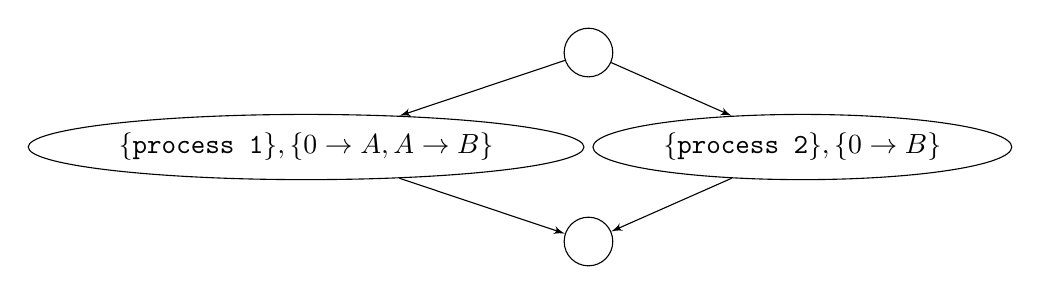
\begin{tikzpicture}[]

% this picture is sadly about 13.5cm. I would want to have 13cm maximum.

\node [draw     , circle                            , text=white             ] (0) {0};
\node [draw=none         , below of=0, yshift=-0.2cm                         ] (x) {};
\node [draw     , ellipse, left  of=x, xshift=0.95cm            , anchor=east] (a) {$\{\texttt{process 1}\}, \{ 0 \rightarrow A, A \rightarrow B \}$};
\node [draw     , ellipse, right of=x, xshift=-0.95cm           , anchor=west] (b) {$\{\texttt{process 2}\}, \{ 0 \rightarrow B \}$};
\node [draw     , circle , below of=x, yshift=-0.2cm, text=white             ] (1) {0};

\path [draw, -latex'] (0) edge (a);
\path [draw, -latex'] (0) edge (b);
\path [draw, -latex'] (a) edge (1);
\path [draw, -latex'] (b) edge (1);

\end{tikzpicture}

	\caption{Concept lattice of function pairs for the example call trees}
	\label{fig:subsumption-example-concept-lattice}
\end{figure}

The proposed \emph{subsumption measure} modifies the previous approach as follows.
The first step is to take the transitive closure $(~)^+$ of the function pair set for each process.
\emph{Transitive closure} of a relation $R \subseteq X \times X$ is commonly defined as:
\begin{equation*}
	\begin{aligned}
		R^+ & := \bigcup_{i \ge 1} R^i \\
		R^1 & := R \\
		R^{j+1} & := R \circ R^j
	\end{aligned}
\end{equation*}
where $j \ge 1$ and $\circ$ denotes the composition of relations, i.e.:
\begin{equation*}
	\begin{aligned}
		S \circ T & := \big\{ (a, c) \in X \times Z \mid ~\text{there exists}~ b \in Y : (a, b) \in T ~\text{and}~ (b, c) \in S \big\}
	\end{aligned}
\end{equation*}
with $S \subseteq Y \times Z$ and $T \subseteq X \times Y$.
This means, function calls with intermediate steps are added to each process's function pair set.
In the example, $0 \rightarrow B$ is added to process~1's set.
Thus, the transitively closed function pair sets for processes~1 and 2 are:
\begin{equation*}
	\begin{aligned}
		\text{functionpairs}(\texttt{process 1})^+ & = \text{functionpairs}(\texttt{process 1}) \cup \{ 0 \rightarrow B \} \\
		\text{functionpairs}(\texttt{process 2})^+ & = \text{functionpairs}(\texttt{process 2})
	\end{aligned}
\end{equation*}
Scalability does not suffer from this step, since the number of function pairs is constant, the transitive closure can be computed for all processes independently, and the size of the resulting lattice does not increase.
Informally, differences between function pair sets cause lattice nodes to be split.
Taking the transitive closure of two function pair sets potentially lessens differences between them, but never creates new differences.
The second step is to construct the lattice the same way as before.
For the example, the resulting lattice is depicted in Figure~\ref{fig:subsumption-example-transitive-concept-lattice}.
\begin{figure}[tb]
	\centering
	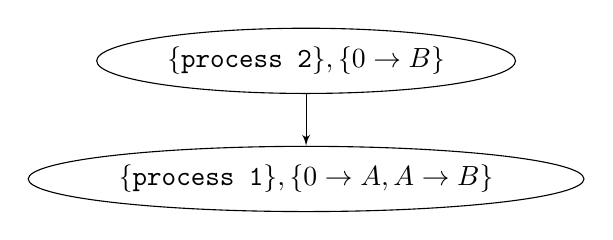
\begin{tikzpicture}[]

\node [draw, ellipse                           ] (0) {$\{\texttt{process 2}\}, \{ 0 \rightarrow B \}$};
\node [draw, ellipse, below of=0, yshift=-0.5cm] (1) {$\{\texttt{process 1}\}, \{ 0 \rightarrow A, A \rightarrow B\}$};

\path [draw, -latex'] (0) edge (1);

\end{tikzpicture}


	\caption{Concept lattice of the transitively closed function pair sets for the example call trees}
	\label{fig:subsumption-example-transitive-concept-lattice}
\end{figure}
The third and last step is to calculate the measure for each pair of process groups.
This approach uses a different measure, a specialisation of the Tversky index~\cite{tversky77}:
\begin{equation*}
	\text{functionpairsubsumption}(P_1, P_2) := \frac{ \mid \text{functionpairs}(P_1)^+ \cap \text{functionpairs}(P_2)^+ \mid }{ \mid \text{functionpairs}(P_2)^+ \mid }
\end{equation*}
If $P_2$'s function pair set is empty, the result is defined to be 1.
For the example, the function pair subsumption measure is 1.
This means that, indeed, process~1 does at least as much work as process~2.
Asking the reverse yields $\frac{1}{3}$, because process~2 calls fewer functions than process~1.
In particular, this means that the measure is not symmetric and, thus, no similarity measure according to the definition.
The modified formula is motivated by the following thoughts:
\begin{itemize}
	\item Imagine scoring subsumption and exclusion element-wise. Subsumption is counted using positive points and exclusion using negative points.
		The measure can, then, be expressed as a fraction of positive points over both positive and negative points.
	\item If $P_2$ carries out work that $P_1$ does not, then this must decrease the measure.
		It, therefore, counts negatively.\vspace{-0.5ex}
	\item If $P_1$ performs work that $P_2$ does not, that is to be ignored.
		Counting them as positives would cause the measure to be arbitrarily close to 1 when $P_1$'s function pair set is much larger than $P_2$'s, despite for example them being disjoint.\vspace{-0.5ex}
	\item Only common function pairs between both sets count positively.
		Therefore, the numerator of the formula is the intersection of both sets.\vspace{-0.5ex}
	\item The denominator is the numerator plus the number of function pairs that $P_2$ alone has.
		In sum, that is the size of $P_2$'s set, possibly overlapping with $P_1$'s.\footnote{$(A \cap B) \cup (B \setminus A) = B$ where $A$ and $B$ are sets}\vspace{-0.5ex}
	\item Thus, if $P_1$'s set includes all of $P_2$'s function pairs, the intersection is the same as $P_2$'s set and the resulting fraction is 1.
\end{itemize}

As a real-world example, take the previous WRF weather simulation (Figure~\ref{fig:wrf-hybrid-16p-concept-lattice} on page~\pageref{fig:wrf-hybrid-16p-concept-lattice}).
Applying the described techniques, yields the concept lattice depicted in Figure~\ref{fig:wrf-hybrid-16p-transitive-concept-lattice}.
Querying it for function pair subsumption, yields that processes~1--4 subsume the threads' function pairs.
One can, therefore, safely assume that these twelve threads perform a subset of the work the processes do.
They are not as different as the 24\% and 30\% similarity in Table~\ref{tab:wrf-hybrid-similarity-matrix} on page~\pageref{tab:wrf-hybrid-similarity-matrix} suggests.
Mind that this conclusion cannot be drawn without transitively closing the function pair sets.
The relation between process~1 and 2--4 does not change, because even without the modification, process~1 subsumes processes~2--4.
\begin{figure}[tb]
	\centering
	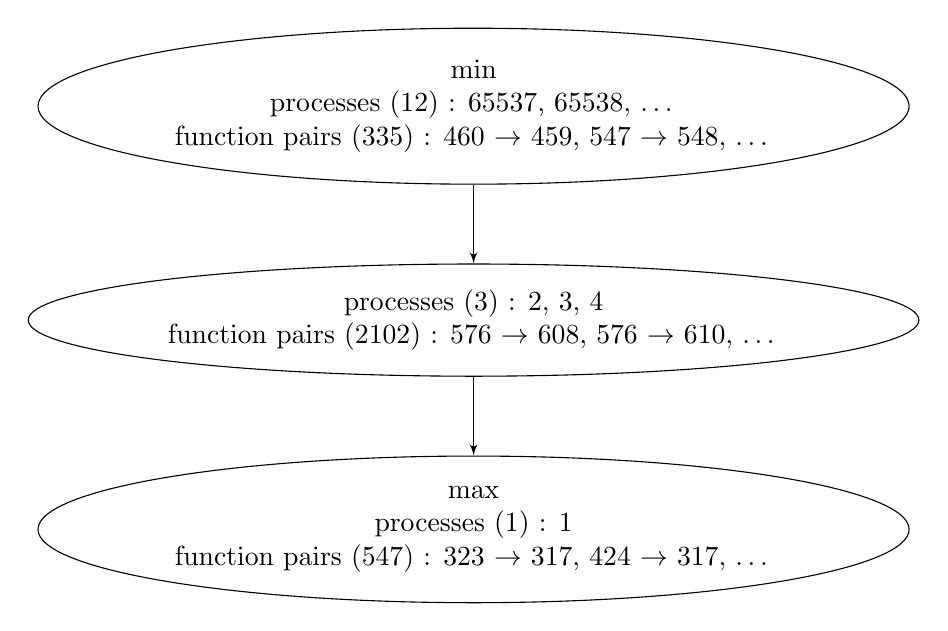
\begin{tikzpicture}[]

\node [draw, ellipse, align=center] (1) {
	min \\
	processes (12) : 65537, 65538, \ldots \\
	function pairs (335) : 460 $\rightarrow$ 459, 547 $\rightarrow$ 548, \ldots
};

\node [draw, ellipse, align=center, below=of 1] (2) {
	processes (3) : 2, 3, 4 \\
	function pairs (2102) : 576 $\rightarrow$ 608, 576 $\rightarrow$ 610, \ldots
};

\node [draw, ellipse, align=center, below=of 2] (3) {
	max \\
	processes (1) : 1 \\
	function pairs (547) : 323 $\rightarrow$ 317, 424 $\rightarrow$ 317, \ldots
};

\path [draw, -latex'] (1)  edge (2);
\path [draw, -latex'] (2)  edge (3);

\end{tikzpicture}

	\caption{Concept lattice of the transitively closed function pair sets for a WRF weather simulation run utilising four processes and twelve threads}
	\label{fig:wrf-hybrid-16p-transitive-concept-lattice}
\end{figure}

The next chapter demonstrates the applicability and scalability of the introduced techniques.
Furthermore, in addition to improving an existing visualisation, a new one leveraging function similarity values is presented.

%%%%%%%%%%%%%%%%%%%%%%%%%%%%%%%%%%%%%%%%%%%%%%%%%%%%%%%%%%%%%%%%%%%%%%%%%%%%%%
\chapter{Evaluation}
\label{sec:evaluation}
This chapter assesses the ability of the introduced techniques to aid software performance analysis and visualisation.
The first two sections evaluate their effectiveness and efficiency.
The third one demonstrates the suitability of the subsumption measure to identify related processes despite apparent differences.
The last part shows how similarity can be used to improve visualisation.

Although this chapter is centred around analysing traces, it is not mandatory to use tracing.
Function or function pair sets can be obtained in many ways including sampling program runs or extracting them from given call trees.
Care has been taken to exclude the effects of tracing in the following evaluation, so that observations, results and conclusions apply regardless of how function pairs are collected.

%%%%%%%%%%%%%%%%%%%%%%%%%%%%%%%%%%%%%%%
\section{Applicability}
\label{sec:evaluation-applicability}
Before evaluating scalability in greater detail, an overview of how the techniques perform on a variety of programs is given.
Table~\ref{tab:many-traces} summarises the results of this broad assessment, which is subsequently discussed.
For each application the concept lattice of function pairs is constructed and then the similarity between all pairs of processes is computed.
\begin{table}[tbh]
	\centering
	\caption{Measured timing and lattice size for selected application traces.}
	\vspace{0.2cm}
	\rowcolors{5}{lightgray}{}
	% \rule{13cm}{3.0pt} % maximum width i wish to use
	% all file sizes have been double checked. all are .z files (except for otf2, there i don't know) files.
	\begin{tabular}{l r r r !{\tablevline} r r r}
		\multicolumn{4}{c !{\tablevline}}{\textbf{Trace} } &
		\multicolumn{3}{c               }{\textbf{Result}} \\

		\multicolumn{1}{c               }{Application    } &
		\multicolumn{1}{c               }{Proc.          } &
		\multicolumn{1}{c               }{$\sim$Size     } &
		\multicolumn{1}{c !{\tablevline}}{Function       } &
		\multicolumn{1}{c               }{$t_{eval}$     } &
		\multicolumn{1}{c               }{Nodes          } &
		\multicolumn{1}{c               }{Groups         } \\

		\multicolumn{1}{c               }{               } &
		\multicolumn{1}{c               }{               } &
		\multicolumn{1}{c               }{(MiB)          } &
		\multicolumn{1}{c !{\tablevline}}{pairs          } &
		\multicolumn{1}{c               }{(ms)           } &
		\multicolumn{1}{c               }{               } &
		\multicolumn{1}{c               }{               } \\

		\hline

		HPL           & 2,360  & 200   &     8 & $<  10$ & 2     & 2  \\ % linpack-deimos-2360p-7tflops % 7 functions
		GROMACS       & 36     & 3,700 & 1,381 & $<  10$ & 24    & 11 \\ % gromacs-mpmd-jens-doleschal-2 % 710 functions
		CCLM          & 180    & 650   &   180 & $<  10$ & 6     & 3  \\ % cclm-cosmo-climate-local-model-180p-24h-weather % 74 functions
		% new measurement is 9ms, CCLM          & 180    & 650   &   180 & $   26$ & 6     & 3  \\ % cclm-cosmo-climate-local-model-180p-24h-weather % 74 functions
		COSMO-SPECS   & 100    & 250   &    50 & $<  10$ & 1     & 1  \\ % cosmo-specs-orig-100p-load-unbalanced % finalize compressed call matrix takes all of that time % 31 functions
		% new measurement is 6ms, COSMO-SPECS   & 100    & 250   &    50 & $   32$ & 1     & 1  \\ % cosmo-specs-orig-100p-load-unbalanced % finalize compressed call matrix takes all of that time % 31 functions
		WRF           & 64     & 300   &   774 & $<  10$ & 2     & 2  \\ % wrf-64p-fpops-l3tcm-io-mem % 561 functions
		FD4           & 65,536 & 1,000 &    55 &     55  & 22    & 14 \\ % fd4-1D-Partitioning-Juqueen_10_64k_final-partbench_065536_m16_gsz01024 % ??? functions
		HOMME         & 1,024  & 200   &   179 & $<  10$ & 3     & 3  \\ % homme-1024p-io-counters-10min-weather % 99 functions
		AMG2006       & 1,024  & 3,700 &   440 &     66  & 11    & 7  \\ % amg2006-filt/1024-proc % finalize compressed call matrix takes all of that time % 207 functions
		IRS           & 64     & 4,250 &   989 &     34  & 18    & 7  \\ % irs-huge % finalize compressed call matrix takes all of that time % 445 functions
		LULESH        & 432    & 350   &   406 &     49  & 182   & 35 \\ % lulesh-432p-hybrid-filt-2iter % 229 functions
		ParaDiS       & 128    & 600   &   649 &  3,486  & 6,367 & 74 \\ % paradis/paradis-2.5.1.1_sk_0128-proc_filt % 325 functions
		PIConGPU      & 39     & 300   &   474 &     11  & 60    & 17 \\ % picongpu-37p-cuda-mpi-pthreads-omp % 280 functions
		BT-MZ         & 16     & 150   &   126 & $<  10$ & 5     & 3  \\ % scorep-bt-mz-16p-B-4x4 % 108 functions
		HPCC MPI-FFTE & 128    & 1,200 &   109 &     70  & 7     & 4  \\ % hpcc-05_mpifft_ice_func % finalize compressed call matrix takes all of that time % 77 functions
		PEPC          & 16,384 & 1,200 &   113 &     15  & 2     & 2  \\ % pepc-16k % ??? functions
	\end{tabular}
	\label{tab:many-traces}
\end{table}

All measurements were done on a notebook featuring an Intel Core i5-2520M processor and dual channel DDR3 PC3-10600 RAM.
For each program run the name of the application and three important parameters of the resulting trace are given.
These three factors namely process count, trace size and total function pair count influence the timing and outcome of applying the techniques.
The number of function pairs lies between the number of functions and its square.
As before, processes include threads and CUDA~\cite{cuda} streams.

For each application the results are depicted on the right side of the table.
The evaluation time $t_{eval}$, the number of nodes in the concept lattice and the number of process groups are of interest.
The evaluation time consists of three steps.
First, add each process's function pairs to the lattice.
After this, finalise the lattice and compute the similarity matrix from it.
It does not include obtaining the function pairs.
Predicting timing is difficult, since it is determined by many factors namely the number of processes to be added, the size and structure of the lattice before each insertion, the number of function pairs to be added in each step and the final lattice's size and structure.
The number of process groups equals the number of nodes with a non-empty process set, and is therefore equal to or smaller than the node count.

The test applications are a selection of benchmarks, pseudo-applications and real-world applications:
\begin{itemize}
	\item HPL~\cite{hpl}, which stands for ``High-Performance Linpack'', is a benchmark that solves systems of linear equations.
		It is used to determine the 500 most powerful, known computers on earth---the TOP500 list~\cite{top500}.\vspace{-0.5ex}
	\item GROMACS~\cite{gromacs, van05}, which stands for ``Groningen Machine for Chemical Simulations'', is a molecular dynamics program specialised in simulating proteins, lipids and nucleic acids.
		It can also be used for non-biological systems, for example polymers.
		GROMACS leverages parallelism using MPI~\cite{mpi}, OpenMP~\cite{openmp} and CUDA.\vspace{-0.5ex}
	\item CCLM~\cite{rockel08}, which stands for ``COSMO Climate Limited-area Modelling'', predicts climate using the COSMO model~\cite{cosmo}.
		COSMO is used, for example, by the Deutscher Wetterdienst to generate weather forecasts.\vspace{-0.5ex}
	\item COSMO-SPECS~\cite{gruetzun08}, improves the accuracy of COSMO's predictions by additionally simulating cloud microphysics.\vspace{-0.5ex}
	\item WRF~\cite{michalakes01, wrf}, which stands for ``The Weather Research \& Forecast Model'' simulates weather, similar to COSMO.\vspace{-0.5ex}
	\item FD4~\cite{lieber, lieber09} stands for ``Four-Dimensional Distributed Dynamic Data structures'' and adds dynamic load balancing to COSMO-SPECS and WRF.
		This particular trace is of a benchmark run that evaluates FD4's scalability.\vspace{-0.5ex}
	\item HOMME~\cite{homme}, which stands for ``High-Order Methods Modeling Environment'', is another weather model.\vspace{-0.5ex}
	\item AMG~\cite{amg}, which stands for ``Algebraic Multigrid Solver'', is a benchmark that solves systems of differential equations.\vspace{-0.5ex}
	\item IRS~\cite{irs}, which stands for ``Implicit Radiation Solver'' benchmarks how suited a computer is to solve systems of diffusion equations.
		AMG2006 and IRS are both part of a benchmark suite compiled at the Lawrence Livermore National Laboratory.\vspace{-0.5ex}
	\item LULESH~\cite{karlin13, lulesh}, which stands for ``Livermore Unstructured Lagrangian Explicit Shock Hydrodynamics'', is a pseudo-application that retains the numerical algorithms, data motion and programming style of a typical hydrodynamics simulation.
		It is used to evaluate the capability of a high performance computer to run such simulations.\vspace{-0.5ex}
	\item ParaDiS~\cite{bulatov04, paradis}, which stands for ``Parallel Dislocation Simulator'', simulates the behaviour of solids under external stress.
		This way one can, for example, predict where cracks appear and how they expand, move and join.\vspace{-0.5ex}
	\item PIConGPU~\cite{bussmann13}, which stands for ``Particle-In-Cell on Graphics Processing Units'', is an implementation of the particle-in-cell method for clusters using NVIDIA graphics cards.
		It simulates the behaviour of charged particles accelerated by a laser.\vspace{-0.5ex}
	\item BT-MZ stands for ``block tri-diagonal multi-zone'' and is a pseudo-application emulating the workload of a typical fluid dynamics simulation.
		The term \emph{multiple zones} means that it uses multiple processes and multithreading for parallelisation.
		BT-MZ is part of the NAS Parallel Benchmarks~\cite{bailey91}.\vspace{-0.5ex}
	\item HPCC MPI-FFTE is a benchmark that performs complex, one-dimensional, discrete Fourier transforms (DFT) using the FFTE package~\cite{ffte}.
		DFT is widely used in digital signal processing, in image processing and to solve partial differential equations.
		MPI-FFTE is included in the HPCC benchmark suite~\cite{luszczek06}.\vspace{-0.5ex}
	\item PEPC~\cite{gibbon04}, which stands for ``Pretty Efficient Parallel Coulomb Solver'', is an $N$-body simulation using an octree as internal representation.
		It simulates the interaction between a laser and charged particles.
\end{itemize}

For each trace, except one, the evaluation time is less than 0.1 second.
Most of the time it is far smaller.
This underlines the applicability of the introduced techniques.
Constructing the lattice for the ParaDiS trace takes a very long 3.226 seconds and calculating the similarity matrix takes the remaining 0.26 seconds.
Most of the time, the number of process groups is below ten.
As expected, group counts vary seemingly independent of the number of processes.
Thus, most applications exhibit fairly regular function call behaviour.
Please note that groups contain processes equal according to the similarity measure.
As indicated in Section~\ref{sec:new-scalability}, the number of steps required to calculate the similarity matrix from a given concept lattice is in $\mathcal{O}(g^2n)$ where $g$ is the number of groups and $n$ the number of nodes in the lattice.
Because of this, the size of the lattice for the ParaDiS run is of concern.

To investigate the findings and concerns more deeply, the next section provides further measurements for two applications, AMG2006 and ParaDiS.

%%%%%%%%%%%%%%%%%%%%%%%%%%%%%%%%%%%%%%%
\section{Scalability}
\label{sec:evaluation-scalability}
This section evaluates the introduced methods in greater detail using two representative applications from the previous section.
The first one is AMG2006, which exhibits a semi-regular function call pattern as a result of employing iterative refinement techniques.
The second one is ParaDiS, where the methods seem to struggle.

To recap, AMG2006 is a benchmark solving systems of differential equations.
ParaDiS simulates solids under external stress.

%%%%%%%%%%%%%%%%%%%
\subsection{Measurement Setup}
\label{sec:evaluation-scalability-measurement}
Every performance measurement was conducted on the computer system Taurus (Figure~\ref{fig:taurus}) at the Technische Universit\"at Dresden.
The partition \emph{sandy} was chosen for all tests.
It features two Intel Xeon E5-2690 processors~\cite{xeone52690} (Sandy Bridge microarchitecture) and 32--128 gibibytes of RAM per motherboard.
Hyper-Threading~\cite{hyperthreading} is disabled system-wide.
Measurements were done using one processor core at a fixed clock rate of 2.9~GHz, without Turbo Boost~\cite{turboboost}.
Even though only one core was used per measurement, the motherboard has been allocated for exclusive access to avoid the influence of other programs running on the same node.
Every measurement was repeated five times and the median of them has been used. Minimum, average and maximum values were monitored for abnormalities.
\begin{figure}[h!]
	\centering
	\includegraphics[width=6.5cm]{taurus}
	\caption{Photo of the high performance computer Taurus, on which scalability testing of the introduced techniques was done}
	\label{fig:taurus}
\end{figure}

%%%%%%%%%%%%%%%%%%%
\subsection{AMG2006}
\label{sec:evaluation-scalability-amg}
The traces generated for the measurements have up to 4,096 processes, are up to 60 gibibytes large, call between 207 and 217 distinct functions and have 436--483 different function pairs.
The discrepancy of function numbers stems from different code paths being taken for different process counts.

Figure~\ref{fig:amg2006-node-and-group-counts} shows the lattice size for increasing process numbers.
\begin{figure}[b!]
	\centering
	% \rule{13cm}{3.0pt} % maximum width i wish to use
	\input{tikz/amg2006-node-counts}
	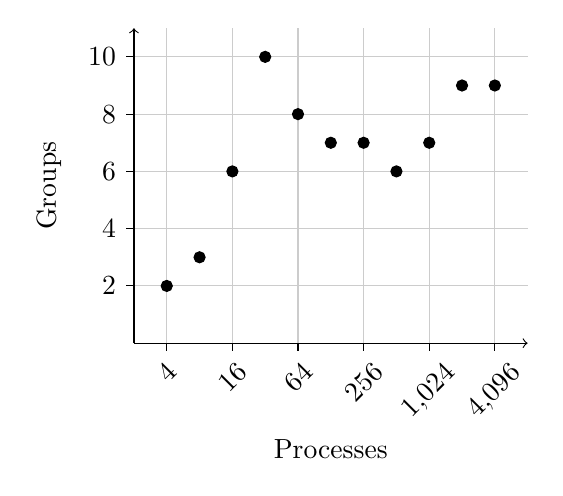
\begin{tikzpicture}[]

\def \xw{5cm}
% \def \xw{4.8cm} % defense slides
\def \xh{4cm}
% \def \xh{2cm} % defense slides

\def \xxmax{12}
\def \xymax{11}

\newcommand{\xx}[1]{#1 / \xxmax * \xw}
\newcommand{\xy}[1]{#1 / \xymax * \xh}

\foreach \x in {1, 3, 5, 7, 9, 11} {
	\draw [lightgray2, thin] (\xx{\x}, 0pt) -- (\xx{\x}, \xy{\xymax}); % x help line
	\draw (\xx{\x}, 0pt) -- (\xx{\x}, -3pt) node[anchor=north] {\rotatebox{45}{\pgfmathparse{2^(\x+1)}\pgfmathprintnumber{\pgfmathresult}}}; % x label
	% \foreach \xa in {0.25, 0.5, 1} { % small log lines
	% 	\pgfmathsetmacro{\xb}{\x - \xa}%
	% 	\draw (\xx{\xb}, 0pt) -- (\xx{\xb}, -2pt);
	% }
}

\foreach \y in {2, 4, 6, 8, 10} {
	\draw[lightgray2, thin] (0pt, \xy{\y}) -- (\xx{\xxmax}, \xy{\y}); % y help line
	\draw (0pt, \xy{\y}) -- (-3pt, \xy{\y}) node[anchor=east] {\y}; % y label
}

\draw[->] (0,0) -- coordinate (x axis mid) (\xw, 0); % x axis
\draw[->] (0,0) -- coordinate (y axis mid) (0  , \xh); % y axis

\node[below=1.1cm] at (x axis mid) {Processes};
\node[left=0.8cm]  at (y axis mid) {\rotatebox{90}{Groups}};

\draw plot[only marks, mark=*] coordinates {
	(\xx{ 1}, \xy{ 2})
	(\xx{ 2}, \xy{ 3})
	(\xx{ 3}, \xy{ 6})
	(\xx{ 4}, \xy{10})
	(\xx{ 5}, \xy{ 8})
	(\xx{ 6}, \xy{ 7})
	(\xx{ 7}, \xy{ 7})
	(\xx{ 8}, \xy{ 6})
	(\xx{ 9}, \xy{ 7})
	(\xx{10}, \xy{ 9})
	(\xx{11}, \xy{ 9})};

\end{tikzpicture}

	\caption{Number of nodes and groups in the concept lattices for AMG2006 runs}
	\label{fig:amg2006-node-and-group-counts}
\end{figure}
One example for such a concept lattice is Figure~\ref{fig:amg2006-512p-concept-lattice} on page~\pageref{fig:amg2006-512p-concept-lattice}.
The time it takes to construct the lattice, finalise it and extract the similarity for each pair of processes is depicted in Figure~\ref{fig:amg2006-lattice-timing}.
\begin{figure}[b!]
	\centering
	% \rule{13cm}{3.0pt} % maximum width i wish to use
	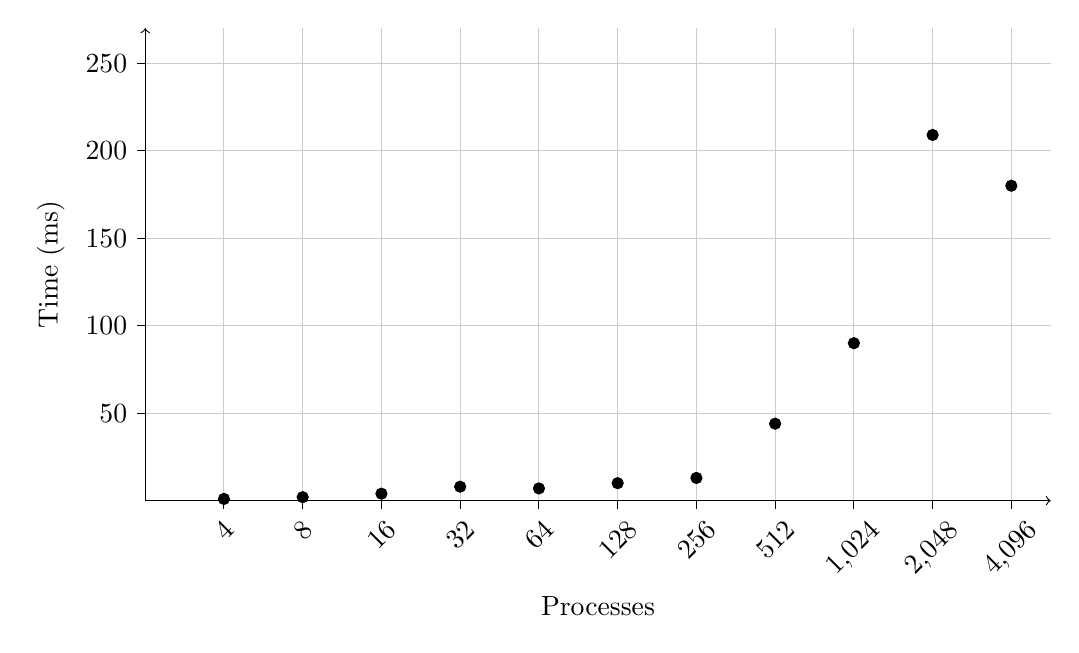
\begin{tikzpicture}[]

\def \xw{11.5cm}
\def \xh{6cm}
% \def \xh{3cm} % defense slides

\def \xxmax{11.5}
\def \xymax{270}

\newcommand{\xx}[1]{#1 / \xxmax * \xw}
\newcommand{\xy}[1]{#1 / \xymax * \xh}

\foreach \x in {1, 2, 3, 4, 5, 6, 7, 8, 9, 10, 11} {
	\draw [lightgray2, thin] (\xx{\x}, 0pt) -- (\xx{\x}, \xy{\xymax}); % x help line
	\draw (\xx{\x}, 0pt) -- (\xx{\x}, -3pt) node[anchor=north] {\rotatebox{45}{\pgfmathparse{2^(\x+1)}\pgfmathprintnumber{\pgfmathresult}}}; % x label
	% \foreach \xa in {0.125, 0.25, 0.5} { % small log lines
	% 	\pgfmathsetmacro{\xb}{\x - \xa}%
	% 	\draw (\xx{\xb}, 0pt) -- (\xx{\xb}, -2pt);
	% }
}

\foreach \y in {50, 100, 150, 200, 250} {
	\draw[lightgray2, thin] (0pt, \xy{\y}) -- (\xx{\xxmax}, \xy{\y}); % y help line
	\draw (0pt, \xy{\y}) -- (-3pt, \xy{\y}) node[anchor=east] {\y}; % y label
}

\draw[->] (0,0) -- coordinate (x axis mid) (\xw, 0); % x axis
\draw[->] (0,0) -- coordinate (y axis mid) (0  , \xh); % y axis

\node[below=1.1cm] at (x axis mid) {Processes};
\node[left=0.9cm]  at (y axis mid) {\rotatebox{90}{Time (ms)}};

\draw plot[only marks, mark=*] coordinates {
	(\xx{ 1}, \xy{  1})
	(\xx{ 2}, \xy{  2})
	(\xx{ 3}, \xy{  4})
	(\xx{ 4}, \xy{  8})
	(\xx{ 5}, \xy{  7})
	(\xx{ 6}, \xy{ 10})
	(\xx{ 7}, \xy{ 13})
	(\xx{ 8}, \xy{ 44})
	(\xx{ 9}, \xy{ 90})
	(\xx{10}, \xy{209})
	(\xx{11}, \xy{180})};

\end{tikzpicture}

	\caption{Timing of the concept lattice construction and evaluation for AMG2006 runs}
	\label{fig:amg2006-lattice-timing}
\end{figure}
Finalising the lattice, i.e. removing redundant function pairs and processes from it, takes almost all of this time.
The rest, i.e. adding each process's function pairs and calculating the similarity matrix at the end, took under four milliseconds for each run.
While iteratively constructing the lattice, van der Merwe's algorithm requires all duplicate function pairs (as shown in Figure~\ref{fig:concept-lattice-example-redundant} on page~\pageref{fig:concept-lattice-example-redundant}) to be present.
Only after constructing the final lattice it is allowed to remove them, so that (as for example in Figure~\ref{fig:concept-lattice-example-not-redundant} on page~\pageref{fig:concept-lattice-example-not-redundant}) each process and function pair is contained exactly once.

The largest number of nodes observed is 36, whereas group counts are at most ten.
There is no definite upward or downward trend.
Numbers vary in an expected fashion.
Different process counts can cause different domain decompositions and therefore different iterative refinement behaviour as well.
It is therefore not surprising that the lattice size is unsteady.
Generally speaking, the techniques are expected to show this kind of differences when changing the number of processes or the problem size.
Observing an upward trend would be concerning.

The time it takes to compute the similarity matrix is expectedly low---at most 209 milliseconds.
As predicted, it seems to depend linearly on the number of processes and is additionally influenced by the size of the lattice.
Particularly, comparing the measurements between 1,024 and 4,096 processes hints at this.
The timing can likely be improved by devising a variant of van der Merwe's algorithm that does not require redundant attributes to be present, through parallelisation, or by fine-tuning the implementation e.g. by reconsidering the choice of containers for internal data storage.

%%%%%%%%%%%%%%%%%%%
\subsection{ParaDiS}
\label{sec:evaluation-scalability-paradis}
The trace files used contain data of up to 4,096 processes, are up to 13 gibibytes large, call between 318 and 325 distinct functions, and have 625--655 different function pairs. Dynamic load balancing has been disabled in ParaDiS.
% Do not say that. Just keep it in mind:
%   Seven more functions were used when running on at least 16 processes.
%   They involve so-called \emph{secondary ghost requests}.

Figures~\ref{fig:paradis-node-counts} and \ref{fig:paradis-group-counts} show the size of the resulting concept lattice for each run.
\begin{figure}[p]
% \begin{figure}[htbp] % defense slides error prevention
	\centering
	% \rule{13cm}{3.0pt} % maximum width i wish to use
	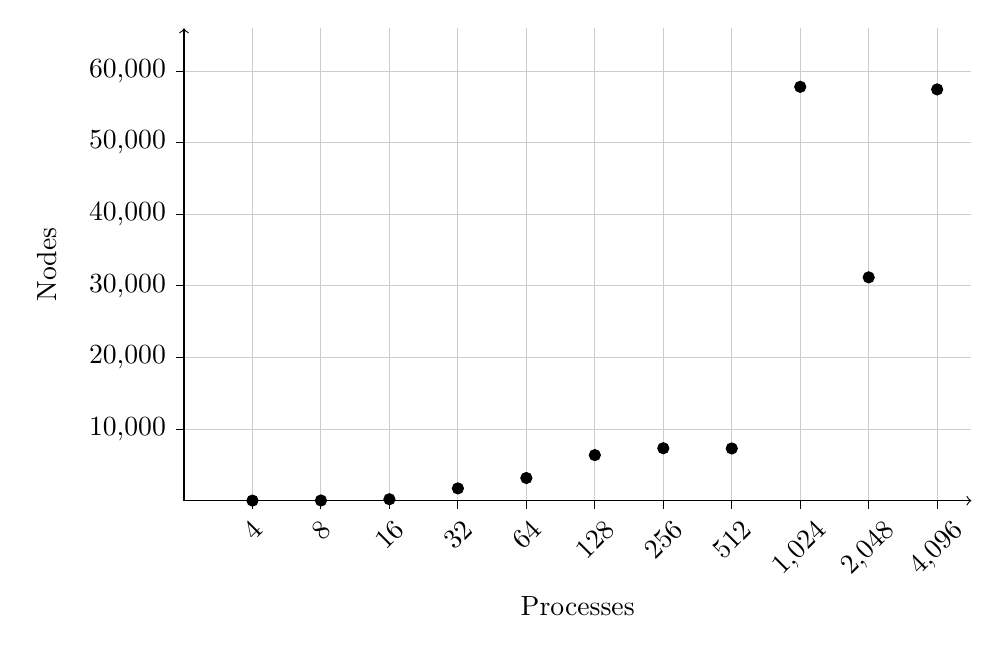
\begin{tikzpicture}[]

% latex tikz (without pgfplots) can only handle values up to 16384. we therefore divide all y values by 1000 and add the missing zeros later on
% the proper way would be to use pgfplots

\def \xw{10cm}
% \def \xw{4.8cm} % defense slides
\def \xh{6cm}
% \def \xh{3.0cm} % defense slides
% \def \xh{2.5cm} % defense slides

\def \xxmax{11.5}
\def \xymax{66}

\newcommand{\xx}[1]{#1 / \xxmax * \xw}
\newcommand{\xy}[1]{#1 / \xymax * \xh}

\foreach \x in {1, 2, 3, 4, 5, 6, 7, 8, 9, 10, 11} {
% \foreach \x in {1, 3, 5, 7, 9, 11} { % defense slides
	\draw [lightgray2, thin] (\xx{\x}, 0pt) -- (\xx{\x}, \xy{\xymax}); % x help line
	\draw (\xx{\x}, 0pt) -- (\xx{\x}, -3pt) node[anchor=north] {\rotatebox{45}{\pgfmathparse{2^(\x+1)}\pgfmathprintnumber{\pgfmathresult}}}; % x label
	% \foreach \xa in {0.125, 0.25, 0.5} { % small log lines
	% 	\pgfmathsetmacro{\xb}{\x - \xa}%
	% 	\draw (\xx{\xb}, 0pt) -- (\xx{\xb}, -2pt);
	% }
}

\foreach \y in {10, 20, 30, 40, 50, 60} {
% \foreach \y in {20, 40, 60} { % defense slides
	\draw[lightgray2, thin] (0pt, \xy{\y}) -- (\xx{\xxmax}, \xy{\y}); % y help line
	\draw (0pt, \xy{\y}) -- (-3pt, \xy{\y}) node[anchor=east] {\y,000}; % y label
}

\draw[->] (0,0) -- coordinate (x axis mid) (\xw, 0); % x axis
\draw[->] (0,0) -- coordinate (y axis mid) (0  , \xh); % y axis

\node[below=1.1cm] at (x axis mid) {Processes};
\node[left=1.5cm]  at (y axis mid) {\rotatebox{90}{Nodes}};

\draw plot[only marks, mark=*] coordinates {
	(\xx{ 1}, \xy{ 0.010})
	(\xx{ 2}, \xy{ 0.026})
	(\xx{ 3}, \xy{ 0.199})
	(\xx{ 4}, \xy{ 1.716})
	(\xx{ 5}, \xy{ 3.168})
	(\xx{ 6}, \xy{ 6.367})
	(\xx{ 7}, \xy{ 7.327})
	(\xx{ 8}, \xy{ 7.297})
	(\xx{ 9}, \xy{57.814})
	(\xx{10}, \xy{31.198})
	(\xx{11}, \xy{57.452})};

\end{tikzpicture}

	\caption{Number of nodes in the concept lattices for ParaDiS runs}
	\label{fig:paradis-node-counts}
\end{figure}
\begin{figure}[p]
% \begin{figure}[htbp] % defense slides error prevention
	\centering
	% \rule{13cm}{3.0pt} % maximum width i wish to use
	\input{tikz/paradis-group-counts}
	\caption{Number of groups for ParaDiS runs}
	\label{fig:paradis-group-counts}
\end{figure}
There are up to 57,814 nodes and 216 groups in a lattice.
The group count is tolerable, whereas the number of nodes is not.
In fact, it is so large that it takes hours to compute the similarity matrix.
Almost all of these nodes neither contain processes nor function pairs.
They are empty.
Nodes like this are necessary for a concept lattice to have for each pair of nodes a unique lowest upper bound and a unique greatest lower bound (see definitions in Section~\ref{sec:new-storage}).
For extracting similarities this property is not strictly necessary.
The described approach traverses the nodes of a concept lattice without using suprema and infima.
Because of this, a new step is added to the techniques.
For each empty node it removes this node and forwards each incoming edge onto all outgoing edges.
The step is invoked after removing redundant information and before computing the similarity matrix.
Implementing this optimisation lowers the node count and, therefore, enables faster similarity matrix computation.
Figure~\ref{fig:paradis-non-empty-node-counts} depicts the number of non-empty nodes for each run.
\begin{figure}[tbh]
	\centering
	% \rule{13cm}{3.0pt} % maximum width i wish to use
	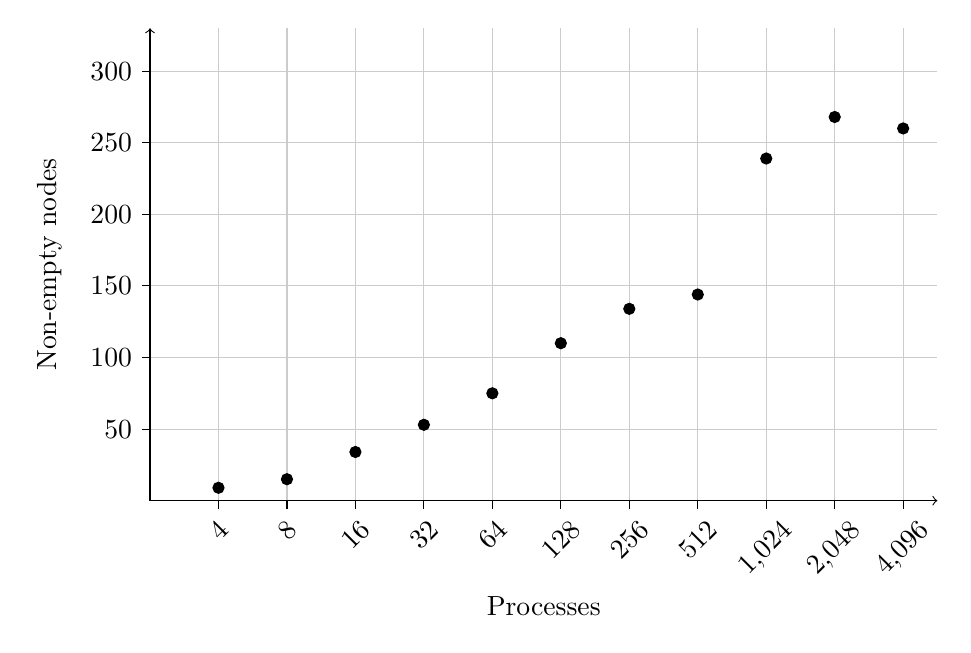
\begin{tikzpicture}[]

\def \xw{10cm}
% \def \xw{4.8cm} % defense slides
\def \xh{6cm}
% \def \xh{2.5cm} % defense slides

\def \xxmax{11.5}
\def \xymax{330}

\newcommand{\xx}[1]{#1 / \xxmax * \xw}
\newcommand{\xy}[1]{#1 / \xymax * \xh}

\foreach \x in {1, 2, 3, 4, 5, 6, 7, 8, 9, 10, 11} {
% \foreach \x in {1, 3, 5, 7, 9, 11} { % defense slides
	\draw [lightgray2, thin] (\xx{\x}, 0pt) -- (\xx{\x}, \xy{\xymax}); % x help line
	\draw (\xx{\x}, 0pt) -- (\xx{\x}, -3pt) node[anchor=north] {\rotatebox{45}{\pgfmathparse{2^(\x+1)}\pgfmathprintnumber{\pgfmathresult}}}; % x label
	% \foreach \xa in {0.125, 0.25, 0.5} { % small log lines
	% 	\pgfmathsetmacro{\xb}{\x - \xa}%
	% 	\draw (\xx{\xb}, 0pt) -- (\xx{\xb}, -2pt);
	% }
}

\foreach \y in {50, 100, 150, 200, 250, 300} {
% \foreach \y in {100, 200, 300} { % defense slides
	\draw[lightgray2, thin] (0pt, \xy{\y}) -- (\xx{\xxmax}, \xy{\y}); % y help line
	\draw (0pt, \xy{\y}) -- (-3pt, \xy{\y}) node[anchor=east] {\y}; % y label
}

\draw[->] (0,0) -- coordinate (x axis mid) (\xw, 0); % x axis
\draw[->] (0,0) -- coordinate (y axis mid) (0  , \xh); % y axis

\node[below=1.1cm] at (x axis mid) {Processes};
\node[left=1.0cm]  at (y axis mid) {\rotatebox{90}{Non-empty nodes}};

\draw plot[only marks, mark=*] coordinates {
	(\xx{ 1}, \xy{  9})
	(\xx{ 2}, \xy{ 15})
	(\xx{ 3}, \xy{ 34})
	(\xx{ 4}, \xy{ 53})
	(\xx{ 5}, \xy{ 75})
	(\xx{ 6}, \xy{110})
	(\xx{ 7}, \xy{134})
	(\xx{ 8}, \xy{144})
	(\xx{ 9}, \xy{239})
	(\xx{10}, \xy{268})
	(\xx{11}, \xy{260})};
	
\end{tikzpicture}


	\caption{Number of non-empty nodes in the concept lattices for ParaDiS runs}
	\label{fig:paradis-non-empty-node-counts}
\end{figure}
It looks very similar to that of the group counts.

As previously stated, van der Merwe's algorithm requires the concept lattice to retain duplicate attributes.
This means that during construction there are no empty nodes which could be removed.
And even if, the algorithm needs an intact concept lattice to work.
Therefore, empty nodes cannot be removed before finalising the lattice.
This in turn means that, unlike for similarity matrix computation, the number of empty nodes still influences the timing of lattice construction.

Figure~\ref{fig:paradis-lattice-timing} depicts the timing of calculating the similarity matrix.
It uses two different time scales to improve readability of the results below 1,024 processes.
\begin{figure}[p]
	\centering
	% \rule{13cm}{3.0pt} % maximum width i wish to use
	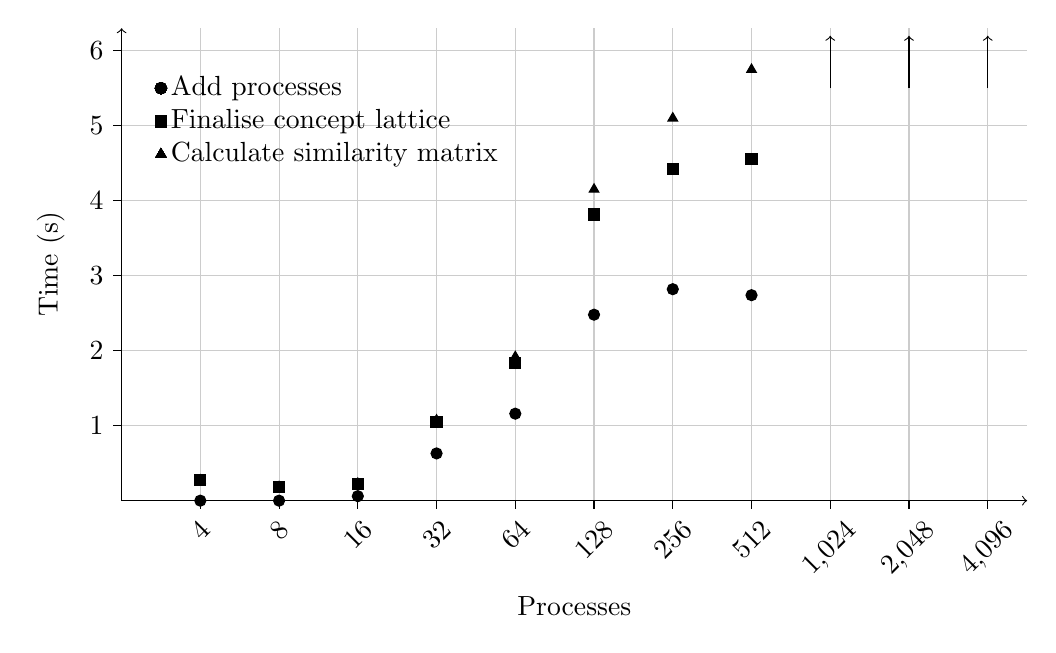
\begin{tikzpicture}[]

\def \xw{11.5cm}
% \def \xw{10.5cm} % defense slides
\def \xh{6cm}
% \def \xh{3.5cm} % defense slides

\def \xxmax{11.5}
\def \xymax{6.3}

\newcommand{\xx}[1]{#1 / \xxmax * \xw}
\newcommand{\xy}[1]{#1 / \xymax * \xh}

\foreach \x in {1, 2, 3, 4, 5, 6, 7, 8, 9, 10, 11} {
	\draw [lightgray2, thin] (\xx{\x}, 0pt) -- (\xx{\x}, \xy{\xymax}); % x help line
	\draw (\xx{\x}, 0pt) -- (\xx{\x}, -3pt) node[anchor=north] {\rotatebox{45}{\pgfmathparse{2^(\x+1)}\pgfmathprintnumber{\pgfmathresult}}}; % x label
	% \foreach \xa in {0.125, 0.25, 0.5} { % small log lines
	% 	\pgfmathsetmacro{\xb}{\x - \xa}%
	% 	\draw (\xx{\xb}, 0pt) -- (\xx{\xb}, -2pt);
	% }
}

\foreach \y in {1, 2, 3, 4, 5, 6} {
	\draw[lightgray2, thin] (0pt, \xy{\y}) -- (\xx{\xxmax}, \xy{\y}); % y help line
	\draw (0pt, \xy{\y}) -- (-3pt, \xy{\y}) node[anchor=east] {\y}; % y label
}

\draw[->] (0,0) -- coordinate (x axis mid) (\xw, 0); % x axis
\draw[->] (0,0) -- coordinate (y axis mid) (0  , \xh); % y axis

\node[below=1.1cm] at (x axis mid) {Processes};
\node[left=0.6cm]  at (y axis mid) {\rotatebox{90}{Time (s)}};

	\draw                         (\xx{0.5},\xy{5.5}) -- plot[mark=*]         (\xx{0.5},\xy{5.5}) -- (\xx{0.5},\xy{5.5}) node[right]{Add processes};
	\draw[yshift=-\baselineskip]  (\xx{0.5},\xy{5.5}) -- plot[mark=square*]   (\xx{0.5},\xy{5.5}) -- (\xx{0.5},\xy{5.5}) node[right]{Finalise concept lattice};
	\draw[yshift=-2\baselineskip] (\xx{0.5},\xy{5.5}) -- plot[mark=triangle*] (\xx{0.5},\xy{5.5}) -- (\xx{0.5},\xy{5.5}) node[right]{Calculate similarity matrix};


\draw plot[only marks, mark=*] coordinates {
	(\xx{ 1}, \xy{ 0   })
	(\xx{ 2}, \xy{ 0   })
	(\xx{ 3}, \xy{ 0.06})
	(\xx{ 4}, \xy{ 0.63})
	(\xx{ 5}, \xy{ 1.16})
	(\xx{ 6}, \xy{ 2.48})
	(\xx{ 7}, \xy{ 2.82})
	(\xx{ 8}, \xy{ 2.74})};
	% (\xx{ 9}, \xy{30.05})
	% (\xx{10}, \xy{14.95})
	% (\xx{11}, \xy{30.2 })};
	
\draw plot[only marks, mark=square*] coordinates {
	(\xx{ 1}, \xy{ 0.272})
	(\xx{ 2}, \xy{ 0.183})
	(\xx{ 3}, \xy{ 0.224})
	(\xx{ 4}, \xy{ 1.049})
	(\xx{ 5}, \xy{ 1.831})
	(\xx{ 6}, \xy{ 3.816})
	(\xx{ 7}, \xy{ 4.422})
	(\xx{ 8}, \xy{ 4.555})};
	% (\xx{ 9}, \xy{50.609})
	% (\xx{10}, \xy{24.478})
	% (\xx{11}, \xy{50.318})};
	
\draw plot[only marks, mark=triangle*] coordinates {
	(\xx{ 1}, \xy{ 0.272})
	(\xx{ 2}, \xy{ 0.183})
	(\xx{ 3}, \xy{ 0.228})
	(\xx{ 4}, \xy{ 1.072})
	(\xx{ 5}, \xy{ 1.918})
	(\xx{ 6}, \xy{ 4.151})
	(\xx{ 7}, \xy{ 5.1  })
	(\xx{ 8}, \xy{ 5.748})};
	% (\xx{ 9}, \xy{57.09 })
	% (\xx{10}, \xy{34.362})
	% (\xx{11}, \xy{58.92})};

\draw [->] (\xx{ 9}, \xy{5.5}) -- (\xx{ 9}, \xy{6.2});
\draw [->] (\xx{10}, \xy{5.5}) -- (\xx{10}, \xy{6.2});
\draw [->] (\xx{11}, \xy{5.5}) -- (\xx{11}, \xy{6.2});

\end{tikzpicture}

	\vspace{2.7cm} \\
	\input{tikz/paradis-lattice-timing-2}
	\caption{Stacked plot of the different concept lattice construction and evaluation phases for ParaDiS runs}
	\label{fig:paradis-lattice-timing}
\end{figure}
Notice that the timing has been split into three phases.
The first one iteratively constructs the lattice.
The second one removes redundant information from it and deletes empty nodes.
The last one computes the similarity matrix from the final lattice.
Mind that the timing of subsequent phases is stacked in the chart.

The time it takes to insert all processes into the lattice mainly depends on the number of processes and the number of nodes in the lattice.
It takes at most 30 seconds for 1,024 processes.
Finalising the lattice, which takes a maximum of 20.5 seconds for 1,024 processes, is influenced by the number of nodes.
Therefore, the timing of these two phases strongly resembles the node count chart (Figure~\ref{fig:paradis-node-counts}).
Computing the similarity matrix, which takes up to 9.9 seconds, depends on the number of non-empty nodes and the group count.
Therefore, calculating the similarity matrix does not take less time for 2,048 processes than for 1,024 and 4,096 as is the case in the previous two phases.

Overall, the number of nodes and groups is much larger than hoped for.
From these measurements, one cannot clearly determine a trend.
It is possible, that the number of nodes and groups increase with rising process counts.
Assuming the techniques are used for grouping similar processes in preparation for further performance analysis, the timing is unacceptable.

Detecting whether the lattice grows too large is simple.
An implementation can set an upper limit for the number of nodes and monitor adherence to it.
The more interesting question is how to alleviate the problem.
One straightforward way is to use functions instead of function pairs for the lattice.
The rest of the techniques is applied without modification.
This yields a coarsening of the grouping.
This means, processes that are equal according to the function pair similarity measure are equal under function similarity measure, as well.
Although being unlikely, the similarity of two unequal processes can decrease when switching to functions.
% example:
%
% 0* 0*
% |  |
% A* A*
% |
% B
% function pairs: 3/4, functions: 2/3
%
% * means self loop

Figures~\ref{fig:paradis-l-node-and-group-counts} and \ref{fig:paradis-l-lattice-timing} depict the lattice size and timing when using functions instead of function pairs.
\begin{figure}[tbp]
	\centering
	%\rule{13cm}{3.0pt} % maximum width i wish to use
	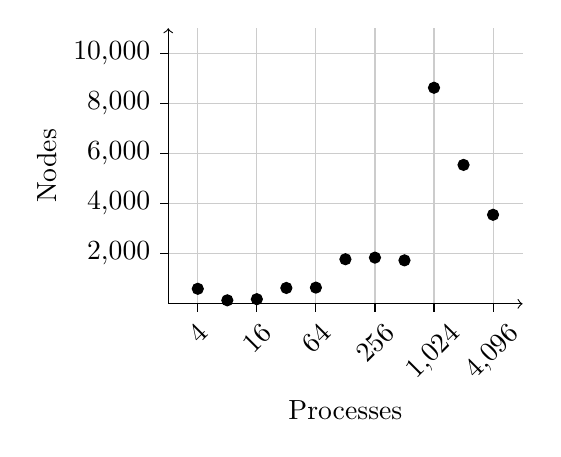
\begin{tikzpicture}[]

\def \xw{4.5cm}
% \def \xw{4.8cm} % defense slides
\def \xh{3.5cm}
% \def \xh{2.5cm} % defense slides

\def \xxmax{12}
\def \xymax{11}

\newcommand{\xx}[1]{#1 / \xxmax * \xw}
\newcommand{\xy}[1]{#1 / \xymax * \xh}

\foreach \x in {1, 3, 5, 7, 9, 11} {
	\draw [lightgray2, thin] (\xx{\x}, 0pt) -- (\xx{\x}, \xy{\xymax}); % x help line
	\draw (\xx{\x}, 0pt) -- (\xx{\x}, -3pt) node[anchor=north] {\rotatebox{45}{\pgfmathparse{2^(\x+1)}\pgfmathprintnumber{\pgfmathresult}}}; % x label
	% \foreach \xa in {0.25, 0.5, 1} { % small log lines
	% 	\pgfmathsetmacro{\xb}{\x - \xa}%
	% 	\draw (\xx{\xb}, 0pt) -- (\xx{\xb}, -2pt);
	% }
}

\foreach \y in {2, 4, 6, 8, 10} {
	\draw[lightgray2, thin] (0pt, \xy{\y}) -- (\xx{\xxmax}, \xy{\y}); % y help line
	\draw (0pt, \xy{\y}) -- (-3pt, \xy{\y}) node[anchor=east] {\y,000}; % y label
}

\draw[->] (0,0) -- coordinate (x axis mid) (\xw, 0); % x axis
\draw[->] (0,0) -- coordinate (y axis mid) (0  , \xh); % y axis

\node[below=1.1cm] at (x axis mid) {Processes};
\node[left=1.3cm]  at (y axis mid) {\rotatebox{90}{Nodes}};

\draw plot[only marks, mark=*] coordinates {
	(\xx{ 1}, \xy{0.6  })
	(\xx{ 2}, \xy{0.14 })
	(\xx{ 3}, \xy{0.185})
	(\xx{ 4}, \xy{0.633})
	(\xx{ 5}, \xy{0.647})
	(\xx{ 6}, \xy{1.779})
	(\xx{ 7}, \xy{1.844})
	(\xx{ 8}, \xy{1.735})
	(\xx{ 9}, \xy{8.624})
	(\xx{10}, \xy{5.545})
	(\xx{11}, \xy{3.554})};

\end{tikzpicture}

	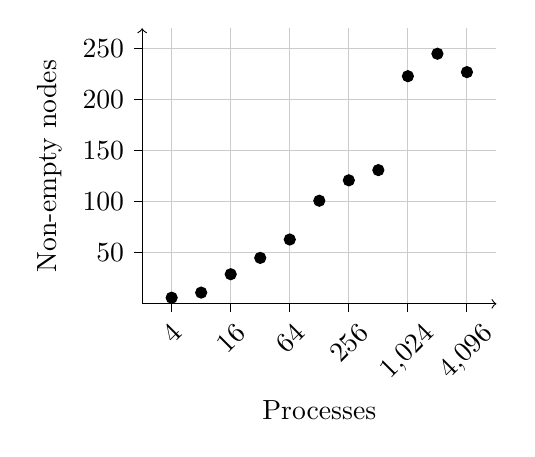
\begin{tikzpicture}[]

\def \xw{4.5cm}
% \def \xw{4.8cm} % defense slides
\def \xh{3.5cm}
% \def \xh{2.5cm} % defense slides

\def \xxmax{12}
\def \xymax{270}

\newcommand{\xx}[1]{#1 / \xxmax * \xw}
\newcommand{\xy}[1]{#1 / \xymax * \xh}

\foreach \x in {1, 3, 5, 7, 9, 11} {
	\draw [lightgray2, thin] (\xx{\x}, 0pt) -- (\xx{\x}, \xy{\xymax}); % x help line
	\draw (\xx{\x}, 0pt) -- (\xx{\x}, -3pt) node[anchor=north] {\rotatebox{45}{\pgfmathparse{2^(\x+1)}\pgfmathprintnumber{\pgfmathresult}}}; % x label
	% \foreach \xa in {0.25, 0.5, 1} { % small log lines
	% 	\pgfmathsetmacro{\xb}{\x - \xa}%
	% 	\draw (\xx{\xb}, 0pt) -- (\xx{\xb}, -2pt);
	% }
}

\foreach \y in {50, 100, 150, 200, 250} {
	\draw[lightgray2, thin] (0pt, \xy{\y}) -- (\xx{\xxmax}, \xy{\y}); % y help line
	\draw (0pt, \xy{\y}) -- (-3pt, \xy{\y}) node[anchor=east] {\y}; % y label
}

\draw[->] (0,0) -- coordinate (x axis mid) (\xw, 0); % x axis
\draw[->] (0,0) -- coordinate (y axis mid) (0  , \xh); % y axis

\node[below=1.1cm] at (x axis mid) {Processes};
\node[left=0.9cm]  at (y axis mid) {\rotatebox{90}{Non-empty nodes}};

\draw plot[only marks, mark=*] coordinates {
	(\xx{ 1}, \xy{6  })
	(\xx{ 2}, \xy{11 })
	(\xx{ 3}, \xy{29 })
	(\xx{ 4}, \xy{45 })
	(\xx{ 5}, \xy{63 })
	(\xx{ 6}, \xy{101})
	(\xx{ 7}, \xy{121})
	(\xx{ 8}, \xy{131})
	(\xx{ 9}, \xy{223})
	(\xx{10}, \xy{245})
	(\xx{11}, \xy{227})};

\end{tikzpicture}

	\\[0.5cm]
	\begin{minipage}{13cm}\raggedright
		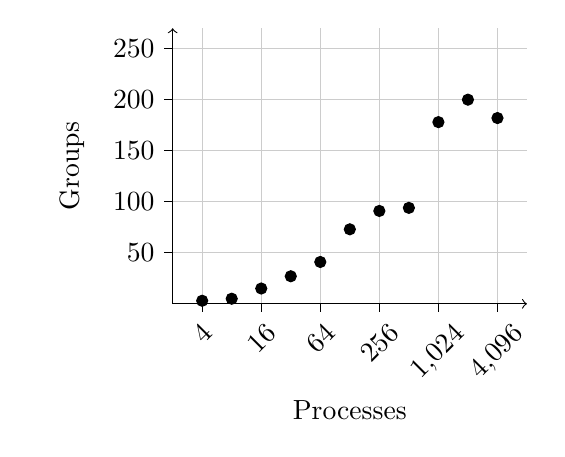
\begin{tikzpicture}[]

\def \xw{4.5cm}
% \def \xw{4.8cm} % defense slides
\def \xh{3.5cm}
% \def \xh{2.5cm} % defense slides

\def \xxmax{12}
\def \xymax{270}

\newcommand{\xx}[1]{#1 / \xxmax * \xw}
\newcommand{\xy}[1]{#1 / \xymax * \xh}

\foreach \x in {1, 3, 5, 7, 9, 11} {
	\draw [lightgray2, thin] (\xx{\x}, 0pt) -- (\xx{\x}, \xy{\xymax}); % x help line
	\draw (\xx{\x}, 0pt) -- (\xx{\x}, -3pt) node[anchor=north] {\rotatebox{45}{\pgfmathparse{2^(\x+1)}\pgfmathprintnumber{\pgfmathresult}}}; % x label
	% \foreach \xa in {0.25, 0.5, 1} { % small log lines
	% 	\pgfmathsetmacro{\xb}{\x - \xa}%
	% 	\draw (\xx{\xb}, 0pt) -- (\xx{\xb}, -2pt);
	% }
}

\foreach \y in {50, 100, 150, 200, 250} {
	\draw[lightgray2, thin] (0pt, \xy{\y}) -- (\xx{\xxmax}, \xy{\y}); % y help line
	\draw (0pt, \xy{\y}) -- (-3pt, \xy{\y}) node[anchor=east] {\y}; % y label
}

\draw[->] (0,0) -- coordinate (x axis mid) (\xw, 0); % x axis
\draw[->] (0,0) -- coordinate (y axis mid) (0  , \xh); % y axis

\node[below=1.1cm] at (x axis mid) {Processes};
\node[left=1.0cm]  at (y axis mid) {\rotatebox{90}{Groups}};
\node[left=1.6cm]  at (y axis mid) {}; % used for alignment with the other figures

\draw plot[only marks, mark=*] coordinates {
	(\xx{ 1}, \xy{3  })
	(\xx{ 2}, \xy{5  })
	(\xx{ 3}, \xy{15 })
	(\xx{ 4}, \xy{27 })
	(\xx{ 5}, \xy{41 })
	(\xx{ 6}, \xy{73 })
	(\xx{ 7}, \xy{91 })
	(\xx{ 8}, \xy{94 })
	(\xx{ 9}, \xy{178})
	(\xx{10}, \xy{200})
	(\xx{11}, \xy{182})};

\end{tikzpicture}


	\end{minipage}
	\caption{Number of nodes, non-empty nodes and groups in the concept lattices for ParaDiS runs using functions instead of function pairs}
	\label{fig:paradis-l-node-and-group-counts}
\end{figure}
\begin{figure}[tbp]
	\centering
	%\rule{13cm}{3.0pt} % maximum width i wish to use
	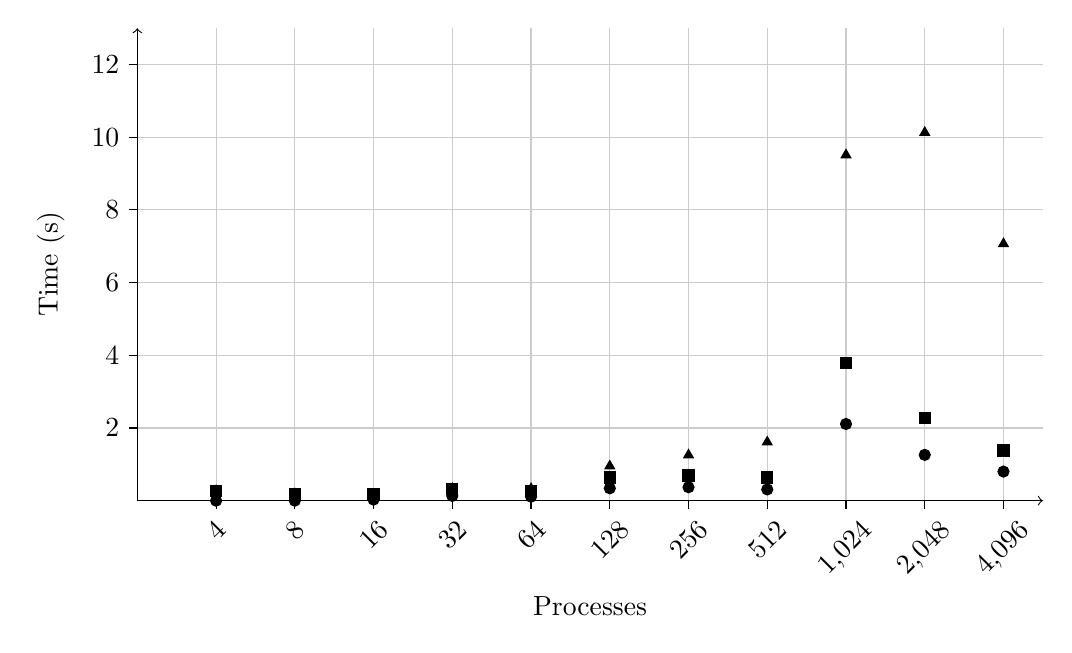
\begin{tikzpicture}[]

\def \xw{11.5cm}
% \def \xw{4.8cm} % defense slides
\def \xh{6cm}
% \def \xh{2.5cm} % defense slides

\def \xxmax{11.5}
\def \xymax{13}

\newcommand{\xx}[1]{#1 / \xxmax * \xw}
\newcommand{\xy}[1]{#1 / \xymax * \xh}

\foreach \x in {1, 2, 3, 4, 5, 6, 7, 8, 9, 10, 11} {
% \foreach \x in {1, 3, 5, 7, 9, 11} { % defense slides
	\draw [lightgray2, thin] (\xx{\x}, 0pt) -- (\xx{\x}, \xy{\xymax}); % x help line
	\draw (\xx{\x}, 0pt) -- (\xx{\x}, -3pt) node[anchor=north] {\rotatebox{45}{\pgfmathparse{2^(\x+1)}\pgfmathprintnumber{\pgfmathresult}}}; % x label
	% \foreach \xa in {0.125, 0.25, 0.5} { % small log lines
	% 	\pgfmathsetmacro{\xb}{\x - \xa}%
	% 	\draw (\xx{\xb}, 0pt) -- (\xx{\xb}, -2pt);
	% }
}

\foreach \y in {2, 4, 6, 8, 10, 12} {
% \foreach \y in {4, 8, 12} { % defense slides
	\draw[lightgray2, thin] (0pt, \xy{\y}) -- (\xx{\xxmax}, \xy{\y}); % y help line
	\draw (0pt, \xy{\y}) -- (-3pt, \xy{\y}) node[anchor=east] {\y}; % y label
}

\draw[->] (0,0) -- coordinate (x axis mid) (\xw, 0); % x axis
\draw[->] (0,0) -- coordinate (y axis mid) (0  , \xh); % y axis

\node[below=1.1cm] at (x axis mid) {Processes};
\node[left=0.8cm]  at (y axis mid) {\rotatebox{90}{Time (s)}};

% 	\draw                         (\xx{0.5},\xy{11}) -- plot[mark=*]         (\xx{0.5},\xy{11}) -- (\xx{0.5},\xy{11}) node[right]{Add processes};
% 	\draw[yshift=-\baselineskip]  (\xx{0.5},\xy{11}) -- plot[mark=square*]   (\xx{0.5},\xy{11}) -- (\xx{0.5},\xy{11}) node[right]{Finalise concept lattice};
% 	\draw[yshift=-2\baselineskip] (\xx{0.5},\xy{11}) -- plot[mark=triangle*] (\xx{0.5},\xy{11}) -- (\xx{0.5},\xy{11}) node[right]{Calculate similarity matrix};

\draw plot[only marks, mark=*] coordinates {
	(\xx{ 1}, \xy{0   })
	(\xx{ 2}, \xy{0   })
	(\xx{ 3}, \xy{0.03})
	(\xx{ 4}, \xy{0.13})
	(\xx{ 5}, \xy{0.11})
	(\xx{ 6}, \xy{0.34})
	(\xx{ 7}, \xy{0.37})
	(\xx{ 8}, \xy{0.31})
	(\xx{ 9}, \xy{2.11})
	(\xx{10}, \xy{1.26})
	(\xx{11}, \xy{0.8 })};

\draw plot[only marks, mark=square*] coordinates {
	(\xx{ 1}, \xy{0.271})
	(\xx{ 2}, \xy{0.184})
	(\xx{ 3}, \xy{0.169})
	(\xx{ 4}, \xy{0.31 })
	(\xx{ 5}, \xy{0.267})
	(\xx{ 6}, \xy{0.64 })
	(\xx{ 7}, \xy{0.691})
	(\xx{ 8}, \xy{0.64 })
	(\xx{ 9}, \xy{3.794})
	(\xx{10}, \xy{2.271})
	(\xx{11}, \xy{1.382})};

\draw plot[only marks, mark=triangle*] coordinates {
	(\xx{ 1}, \xy{ 0.271})
	(\xx{ 2}, \xy{ 0.184})
	(\xx{ 3}, \xy{ 0.172})
	(\xx{ 4}, \xy{ 0.327})
	(\xx{ 5}, \xy{ 0.327})
	(\xx{ 6}, \xy{ 0.95 })
	(\xx{ 7}, \xy{ 1.255})
	(\xx{ 8}, \xy{ 1.611})
	(\xx{ 9}, \xy{ 9.511})
	(\xx{10}, \xy{10.129})
	(\xx{11}, \xy{ 7.066})};

\end{tikzpicture}

	\caption{Stacked plot of the different concept lattice construction and evaluation phases for ParaDiS runs using functions instead of function pairs}
	\label{fig:paradis-l-lattice-timing}
\end{figure}
The trends are, as expected, similar to the function pair variant.
While the number of nodes decreases to roughly 15\% of the function pair lattice, the number of non-empty nodes and groups is only slightly less.
The maximum number of nodes is 8,624, the largest number of non-empty nodes is 245 for 2,048 processes and the maximum group count is 200 for 2,048 processes.
As expected from these numbers, adding processes and finalising the concept lattice is significantly faster.
Adding processes takes up to 2.1 seconds.
Finalisation takes at most 1.7 seconds.
Since the number of non-empty nodes and groups is only a little less, computing the similarity matrix improves just slightly.
A maximum of 7.9 seconds is measured.

While the node count is much lower than in the function pair variant, the number of non-empty nodes and groups improved only slightly.
The upside is that the resulting groups are almost the same as in the function pair case.
In an implementation, it is advisable to construct both, the function and function pair lattice, at the same time and pick one (or neither) upon hitting a set limit of nodes or groups.
Using this variant, the time required to compute the similarity matrix is lowered from 58.9 to 10.1 seconds for the worst-case.
If a performance analysis tool is only interested in the grouping and not the specific similarity values, the needed time is lowered from 50.6 down to 3.8 seconds.

There are two other ways to improve scalability.
The first one is to filter functions on demand.
While iteratively constructing the concept lattice, the implementation can monitor the number of nodes.
When the insertion of a particular process causes the node count to increase steeply, the implementation can repeat the insertion excluding attributes causing the blow-up.
Alternatively, it redoes the whole construction omitting them completely.
The difference between the two is that the former one is faster but some attributes are not added to all processes that should have them, which might be undesirable.
By removing functions or function pairs, information about program structure is lost.
Therefore, one has to plan for this loss of accuracy and/or retain important information.

The second approach is to use hashing.
It is viable only if the process grouping and no specific similarity values are needed.
For each process the canonical form of the function pair set is hashed and inserted into a hash table.
The set itself can be discarded.
This yields the same equalities as before.
Hash collisions introduce false positives.
The likelihood of negative effect can be decreased by using a strong hash function.
Compared to the techniques presented in this thesis the hashing approach can only detect equality but is extremely fast, requires less memory and can be parallelised easily.

The next section explains why lattice-based similarity fails for ParaDiS.
It generalises the findings and discusses implications.

%%%%%%%%%%%%%%%%%%%
\subsection{Irregular Function Call Patterns}
\label{sec:evaluation-scalability-irregular}
Programs exhibit regular function call patterns~\cite{allineaddt, arnold07, johnson91}.
This is especially true for the dominant style of parallel programming \emph{single program multiple data}~\cite{spmd}.
Which functions are called on which process and in which order is largely independent of the process count and problem size.
However, this is not entirely true.
Two classes of applications have been identified that have substantial differences in the code paths taken between different processes.
ParaDiS fits into one of them.

A \emph{scheduler} is a mechanism distributing tasks to processes, e.g. to optimise resource usage.
Different functions encapsulate different tasks.
The process on which a function then runs is practically random from the perspective of the performance analysis tool.
This is, for example, the case for CUDA streams.
A graphics card is assigned one or more streams.
A scheduler dynamically assigns work packages to streams at runtime.
Generally, two runs of the same program do not produce the same function or function pair sets for the streams.
For the same reason, comparing two streams inside one run yields random differences.
Consequently, the results of the techniques are unpredictable, if the analysed application implements scheduling.

Imagine an application using domain decomposition, where every process simulates one or more cells of a three-dimensional grid.
On this grid a number of objects, for examples planets, stars, lasers, spaceships and explosions are placed.
Simulating a time step for an object invokes object-specific functions.
Objects interact with each other and travel between cells as the simulation progresses.
The functions a process calls, then, depend on the spatial position of each object.
The described scenario can also use dynamic load balancing and, therefore, reassign objects between processes at runtime.
Comparing two runs or two processes inside one run can yield differences that the techniques of this thesis cannot process effectively.
ParaDiS is such an application.
The execution of code paths on a process depends on the domain decomposition and the location and state of each object.

In both cases, the effects also depend on the total execution time of the program.
The longer an application runs, e.g. the more time steps it simulates, the more similar the function and function pair sets can get.
The opposite is less likely but possible.

To conclude this section, it can be stated that the introduced similarity methods are unsuited for the described application types.
Fortunately, these programs represent a minority and there exists a number of remedies.
For example, one can filter functions, or use hashing as described at the end of the previous section.
Another possibility is to combine irregular processes into one and apply the techniques to the combined process and the regularly behaving ones.
Depending on the situation this approach might be acceptable.

The next section evaluates the suitability of the subsumption measure to detect a special class of differences using two applications.

%%%%%%%%%%%%%%%%%%%%%%%%%%%%%%%%%%%%%%%
\section{Subsumption Measure}
\label{sec:evaluation-subsumption}
Section~\ref{sec:new-subsumption} introduced a variant of the similarity measure that is robust to fluctuations in function call patterns due to the omission of calls.
If two processes are dissimilar according to function pair similarity, it might still be the case that they are similar, but some functions are missing or some invocations have been inlined.
First, this section demonstrates the effectiveness of the subsumption measure for detecting threads.
Second, the measure is used to identify granularity differences between traces of different processes.

\begin{figure}[h]
	% \rule{13cm}{3.0pt} % maximum width i wish to use
	% traces/scorep-bt-mz-16p-B-4x4
	\centering
	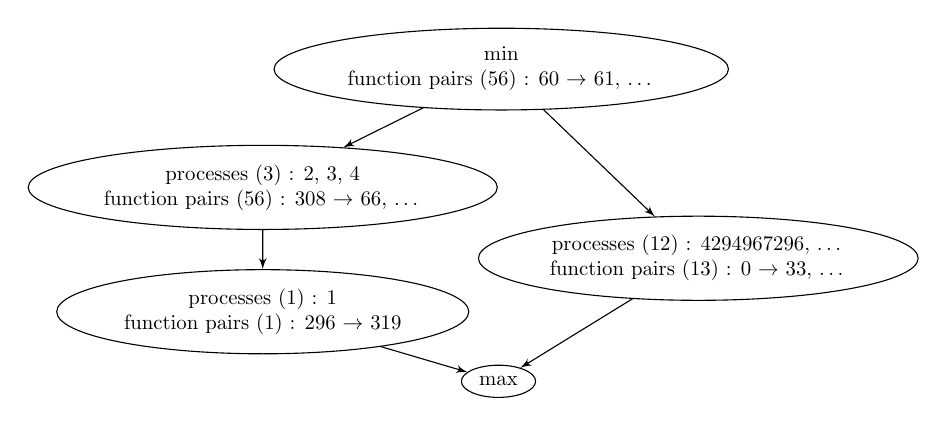
\begin{tikzpicture}[scale=0.75, every node/.style={scale=0.75}]

\node [draw, ellipse, align=center] (min) {
	min \\
	function pairs (56) : 60 $\rightarrow$ 61, \ldots};

\node [draw, ellipse, align=center, below left=0cm of min, xshift=1.5cm, yshift=-1cm] (l) {
	processes (3) : 2, 3, 4 \\
	function pairs (56) : 308 $\rightarrow$ 66, \ldots};

\node [draw, ellipse, align=center, below=0.5cm of l] (ll) {
	processes (1) : 1 \\
	function pairs (1) : 296 $\rightarrow$ 319};

\node [draw, ellipse, align=center, right=0.5cm of l, xshift=-1cm, yshift=-1.2cm] (r) {
	processes (12) : 4294967296, \ldots \\
	function pairs (13) : 0 $\rightarrow$ 33, \ldots};

\node [draw, ellipse, below right=0.5cm of ll, xshift=0.6cm] (max) {max};

\path [draw, -latex'] (min) edge (l);
\path [draw, -latex'] (min) edge (r);
\path [draw, -latex'] (l)   edge (ll);
\path [draw, -latex'] (ll)  edge (max);
\path [draw, -latex'] (r)   edge (max);

\end{tikzpicture}


	\caption{Concept lattice of function pairs for a BT fluid dynamics simulation run utilising four processes and twelve threads}
	\label{fig:bt-16p-concept-lattice}
\end{figure}
\begin{table}[b]
	\centering
	\caption{Similarity matrix for a BT fluid dynamics simulation run utilising four processes and twelve threads}
	\vspace{0.2cm}
	\begin{tabular}{r | r r r}
						& Process 1 & Process 2, 3, 4 & Threads \\
		\hline
		Process 1       &    1      & 0.99            & 0.44    \\
		Process 2, 3, 4 & 0.99      &    1            & 0.45    \\
		Threads         & 0.44      & 0.45            &    1    \\
	\end{tabular}
	\label{tab:bt-similarity-matrix}
\end{table}
In Section~\ref{sec:new-subsumption} the capability of the approach for detecting spawned threads has already been demonstrated for the WRF weather simulation.
A second instance, using the pseudo-application BT, is presented here.
As mentioned in Section~\ref{sec:evaluation-applicability}, BT imitates the computation of a typical fluid dynamics simulation and solves systems of partial differential equations for this purpose.
It uses MPI and OpenMP for parallelisation.
Figure~\ref{fig:bt-16p-concept-lattice} shows the regular concept lattice for the BT run, which executes on four processes and twelve threads.
To recap, each node contains a set of processes and function pairs.
The size of the set is in parenthesis and a few example entries follow.
Each node inherits the function pair sets from nodes reachable along upward-edges.
In this run, processes have the identifiers 1 to 4, whereas threads are 4,294,967,296 ($= 2^{32}$) and above.
All processes and threads share 56 function pairs.
Process~1 has one additional pair compared to processes~2--4 and, thus, subsumes them even before taking the transitive closure of their function sets.
Threads differ from processes.
Table~\ref{tab:bt-similarity-matrix} depicts the resulting similarity values.
Remember, similarity is symmetric and returns 100\% when comparing something to itself.

Transitively closing all function pair sets and constructing the lattice anew yields the concept lattice (Figure~\ref{fig:bt-16p-transitive-concept-lattice}) from which the subsumption measure for each pair of processes/threads is subsequently computed.
Now, the threads are indeed identified as having a subset of the processes' function pairs, since their node is reachable along upward-edges starting at the processes.
Table~\ref{tab:bt-subsumption-metric-matrix} shows the resulting subsumption measure matrix.
The cells represent the likelihood of the process/thread in the row doing at least as much work as the one in the corresponding column.
The main diagonal is always 1.
Process~1 has all function pairs, possibly using intermediate steps, of every other process and thread (100\%).
One can therefore conjecture that process 1 does at least as much work as the other processes and threads.
Processes~2--4 subsume the threads (100\%).
The opposite is unlikely since the subsumption measure is 31\%.
Process~1 is more likely to subsume processes~2--4 than the opposite being the case (99\% < 100\%), but they are very similar.
In fact, process~1 calls the extra function \texttt{print\_results}.
\begin{figure}[t]
	% \rule{13cm}{3.0pt} % maximum width i wish to use
	% traces/scorep-bt-mz-16p-B-4x4
	\centering
	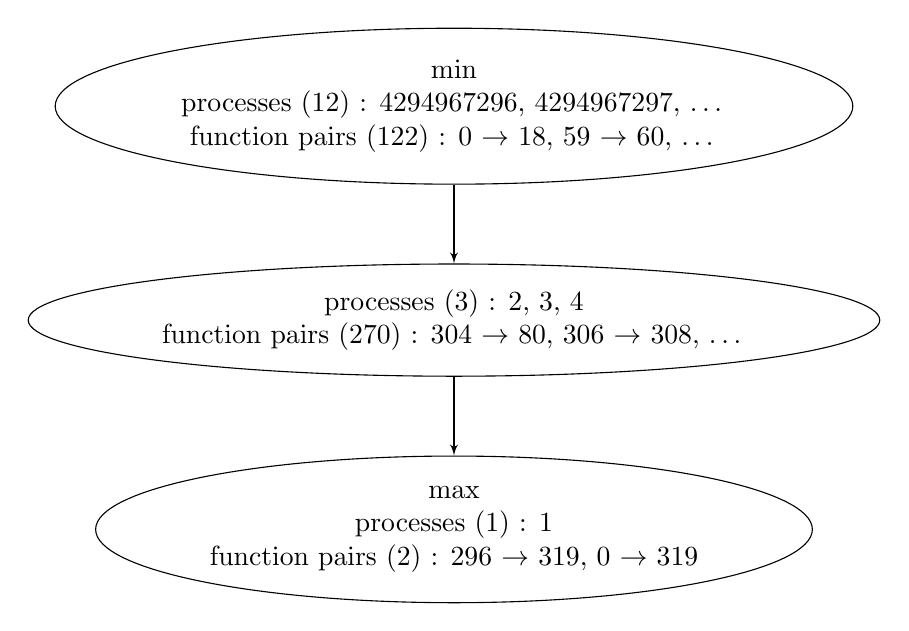
\begin{tikzpicture}[]

\node [draw, ellipse, align=center] (1) {
	min \\
	processes (12) : 4294967296, 4294967297, \ldots \\
	function pairs (122) : 0 $\rightarrow$ 18, 59 $\rightarrow$ 60, \ldots
};

\node [draw, ellipse, align=center, below=of 1] (2) {
	processes (3) : 2, 3, 4 \\
	function pairs (270) : 304 $\rightarrow$ 80, 306 $\rightarrow$ 308, \ldots
};

\node [draw, ellipse, align=center, below=of 2] (3) {
	max \\
	processes (1) : 1 \\
	function pairs (2) : 296 $\rightarrow$ 319, 0 $\rightarrow$ 319
};

\path [draw, -latex'] (1)  edge (2);
\path [draw, -latex'] (2)  edge (3);

\end{tikzpicture}

	\caption{Concept lattice of the transitively closed function pair sets for a BT fluid dynamics simulation run utilising four processes and twelve threads}
	\label{fig:bt-16p-transitive-concept-lattice}
\end{figure}
\begin{table}[b]
	\centering
	\caption{Subsumption measure matrix for a BT fluid dynamics simulation run utilising four processes and twelve threads}
	\vspace{0.2cm}
	\begin{tabular}{r | r r r}
						& Process 1 & Process 2, 3, 4 & Threads \\
		\hline
		Process 1       &    1      &    1            & 1       \\
		Process 2, 3, 4 & 0.99      &    1            & 1       \\
		Threads         & 0.31      & 0.31            & 1       \\
	\end{tabular}
	\label{tab:bt-subsumption-metric-matrix}
\end{table}

Mind, that the call trees of the threads are not sub-trees of the processes'.
Therefore, straightforward call tree comparison does not yield the above results.
The same holds when using function pair sets.
Taking the transitive closure of each set is key.

\begin{figure}[p]
	% gromacs-mpmd-jens-doleschal-1
	\centering
	\includegraphics[width=13.08cm]{gromacs-call-tree}
	\vspace{2cm} \\
	\includegraphics[width=13.08cm]{gromacs-process-timeline}
	\caption{Call tree excerpts and Vampir Process Timelines of the four master threads with decreasing detail from left to right / top to bottom. Application-specific functions are depicted in green. OpenMP regions and functions are brown. MPI functions are red. CUDA functions turquoise.}
	\label{fig:gromacs-call-tree-and-process-timeline}
\end{figure}
Another use for this approach is to detect whether differences between processes across two runs, or equally inside one run, are due to inlining or different levels of recording granularity.
For example, rarely are the full execution details needed for every process.
One representative might be enough.
To evaluate the effectiveness of the subsumption techniques, the molecular dynamics simulator GROMACS is used.
The program run executes on four processes, each spawning five threads and three CUDA streams.
Each process has its own executable with different built-in instrumentation.
From process~1 to 4, the recording detail decreases.
The first process records the most, the second one a little less.
The third one only records OpenMP, MPI and CUDA calls.
Process 4 observes only MPI and CUDA.
To provide more context, Figure~\ref{fig:gromacs-call-tree-and-process-timeline} shows an excerpt of the call tree and function call stack over time for each process, called \emph{master thread} from here on.

Creating the lattice and computing the subsumption measure matrix (Table~\ref{tab:gromacs-m-subsumption-measure-matrix}) does not yield what one would expect.
Master thread~0 is identified to subsume master thread~1, but master thread~2 and 3 still show substantial differences (63\% and 50\%).
Due to an implementation detail in the trace recording software Score-P~\cite{scorep10}, a new artificial main function called \texttt{PARALLEL} is introduced when only recording OpenMP, MPI and CUDA events or less.
This function lies at the lowest call stack level and calls each recorded function.
Therefore, master thread 2 and 3 are not correctly identified as subsumed by master thread~0 and 1.
This problem can easily be fixed via string matching.
The preferred way would be to remove this artificial function from Score-P.
\begin{table}[tb]
	\centering
	\caption{Function-pair-based subsumption measure matrix for the four master threads of a GROMACS simulation run}
	\vspace{0.2cm}
	\begin{tabular}{r | r r r r}
						& MT:0 & MT:1 & MT:2 & MT:3 \\
		\hline
		Master thread:0 & 1    & 1    & 0.63 & 0.5  \\
		Master thread:1 & 0.73 & 1    & 0.63 & 0.5  \\
		Master thread:2 & 0.05 & 0.07 & 1    & 1    \\
		Master thread:3 & 0.01 & 0.01 & 0.24 & 1    \\
	\end{tabular}
	\label{tab:gromacs-m-subsumption-measure-matrix}
\end{table}
\begin{table}[tb]
	\centering
	\caption{Function-based subsumption measure matrix for the four master threads of a GROMACS simulation run}
	\vspace{0.2cm}
	\begin{tabular}{r | r r r r}
						& MT:0 & MT:1 & MT:2 & MT:3 \\
		\hline
		Master thread:0 & 1    & 1    & 0.99 & 0.98 \\
		Master thread:1 & 0.76 & 1    & 0.99 & 0.98 \\
		Master thread:2 & 0.24 & 0.31 & 1    & 1    \\
		Master thread:3 & 0.08 & 0.10 & 0.33 & 1    \\
	\end{tabular}
	\label{tab:gromacs-l-subsumption-measure-matrix}
\end{table}

Calculating the subsumption measure for the functions instead of function pairs yields the expected results (Table~\ref{tab:gromacs-l-subsumption-measure-matrix}).
The four upper-right cells are not 100\% due to this one extra function.

As demonstrated using three real-world applications, the subsumption approach is an effective tool for detecting spawned threads, different levels of recording granularity and inlining.
This information is valuable for further comparative performance analysis.
The next section evaluates how the introduced similarity techniques can aid performance visualisation.

%%%%%%%%%%%%%%%%%%%%%%%%%%%%%%%%%%%%%%%
\section{Visualisation}
\label{sec:evaluation-visualisation}
The function and function pair similarity measures are intended to be a low-overhead, early filtering mechanism that automatically clusters processes according to their structure.
As an auxiliary tool, the subsumption measure finds out what causes differences discovered by the similarity measure.
It answers questions like: ``Are processes~2 to 4 different from process~1, because process~1 additionally prints debug output and writes to log files?'', or ``Are threads 1--4 spawned from process~1?''.
The concept lattice is an efficient way of storing the information needed to determine the similarity or subsumption measure for each pair of processes.

\begin{figure}[b!]
	% traces/wrf_0016cpus_hybrid_counter
	\centering
	\includegraphics[width=7.7cm]{wrf-hybrid-16p-user-presentable-concept-lattice} % 7.7cm = 13.0 / 667px * 395px
	\caption{User-friendly version of Figure~\ref{fig:wrf-hybrid-16p-concept-lattice} on page~\pageref{fig:wrf-hybrid-16p-concept-lattice}, based on the concept lattice of function pairs for a WRF weather simulation run, annotated with function groups and condensed process names. The run utilises four processes and twelve threads. Percentages depict the amount of new function pairs a node introduces.}
	\label{fig:wrf-hybrid-16p-user-presentable-concept-lattice}
\end{figure}
Visualising the lattice itself works for cases with a sufficiently small number of nodes.
Annotating the concept lattice with information about applied parallel programming paradigms and APIs yields a useful tool for program structure inspection.
Using the WRF weather simulation, Figure~\ref{fig:wrf-hybrid-16p-user-presentable-concept-lattice} shows what this new tool could look like.
Unfortunately not all application runs yield low lattice node counts, as is demonstrated in the previous sections.
No mechanism for reducing the number of nodes to arbitrarily small levels whilst preserving important information exists, yet.
Therefore, visualising the lattice in an automated way is not recommended.
Instead, the introduced techniques should be incorporated into existing visualisations or used to develop new ones on top of it.
The following two sections demonstrate the applicability of the methods to aid visualisation.
First, they are applied to improve an existing Vampir display.
Second, a novel profile view is proposed which leverages the introduced clustering.

%%%%%%%%%%%%%%%%%%%
\subsection{Improving Vampir's Process Summary}
\label{sec:evaluation-visualisations-process}
\begin{figure}[b!]
	% traces/pi-ring-100p-hybrid
	\centering
	\includegraphics[width=13.08cm]{pi-ring-100p-hybrid-process-summary}
	\caption{Vampir's Master Timeline, Function Summary and Process Summary for an example program computing decimal places of $\pi$ using MPI and OpenMP. The run utilises ten processes and 90 threads.}
	\label{fig:pi-ring-100p-hybrid-process-summary}
\end{figure}
Vampir's Process Summary display is first introduced in Section~\ref{sec:background-clustering}.
Figure~\ref{fig:pi-ring-100p-hybrid-process-summary} gives another example of its visualisation.
Aside from the Process Summary at the bottom, the Master Timeline and Function Summary are depicted to provide some context.
Subsequently, an overview of the display, which is described in greater detail by Brunst~\cite{brunst07}, is given.
The Process Summary presents a clustered per-process Function Summary.
The $k$-means algorithm~\cite{forgy65, lloyd82, macqueen67, steinhaus56} determines the clustering.
It generates a clustering of $p$ $d$-dimensional points for a target number of clusters $k$ in $\mathcal{O}(p^{dk+1} \log p)$ steps.
The display uses a fixed number of dimensions, which are the ten functions having the overall largest accumulated exclusive time.
Each process is a point in this ten-dimensional space with coordinates corresponding to the accumulated exclusive times of the respective functions in this process.
The number of clusters is, by default, determined by the available vertical space in the chart.
Users can also set this number manually.
For each cluster the display shows (from left to right) the number of processes in this cluster, a simple graphical representation of the position of these processes and a stacked bar chart.
The stacked bar chart has one bar for each of the ten functions.
Each bar has a staircase representation marking the minimum, average and maximum accumulated exclusive time of all processes in this cluster.
The added length of all bars is of little interest, since it is the summed maxima from different processes.
In conclusion, the Process Summary presents an overview of the time each process spends in the ten most time-consuming functions.
It gives insight into a program's structure by scalably clustering processes according to their profile.
The clustering minimises variation of the shown numbers in each cluster.

The effects of replacing the current clustering approach with the new techniques is illustrated, subsequently.
First, an application calculating the decimal places of $\pi$, utilising ten processes and 90 threads, is used.
It employs MPI and OpenMP to run in parallel.
Figure~\ref{fig:pi-ring-100p-hybrid-new-clustering} shows the result of applying function pair similarity grouping to the Process Summary.
\begin{figure}[tb]
	% traces/pi-ring-100p-hybrid
	\centering
	\includegraphics[width=13cm]{pi-ring-100p-hybrid-new-clustering}
	\caption{Vampir's Process Summary using the new methods to generate clusters for a $\pi$ example program run}
	\label{fig:pi-ring-100p-hybrid-new-clustering}
\end{figure}
All ten processes are in one cluster, whereas the threads form the second cluster.
Using fixed two clusters, the current approach yields the clustering depicted in Figure~\ref{fig:pi-ring-100p-hybrid-old-clustering}.
\begin{figure}[tb]
	% traces/pi-ring-100p-hybrid
	\centering
	\includegraphics[width=13cm]{pi-ring-100p-hybrid-old-clustering}
	\caption{Vampir's Process Summary using the current clustering to create two clusters for a $\pi$ example program run}
	\label{fig:pi-ring-100p-hybrid-old-clustering}
\end{figure}
Interestingly, it mixes threads and processes, even though they do not call the same functions.
Mind that \texttt{MPI\_Recv} and \texttt{tracing} are absent on the threads.
This occurs, because the variations in execution time of the OpenMP barrier and parallel region are larger than the difference between non-existent (zero) and actual \texttt{MPI\_Recv} and \texttt{tracing} timings.
If one process in a cluster does not call a function, the corresponding bar's minimum defaults to zero.
The current approach, thus, hides some of the variation in OpenMP barrier and parallel region timings of cooperating and functionally equal processes/threads.
Using the new methods, on the other hand, reveals more relevant variations, gives better minima and overall yields a more meaningful clustering.

Figure~\ref{fig:fd4-4096p-old-clustering} shows the clustering for a large FD4 trace using the current approach.
For such a highly parallel, homogeneous application the resulting clusters seem to be random.
Applying the new methods (Figure~\ref{fig:fd4-4096p-new-clustering}) reduces the number of clusters to two.
One cluster contains the first and last process.
The other processes form the second cluster.
In this case, it is not obvious what the more meaningful approach is.
Displaying more or fewer clusters does not reveal any more information.
Showing a limited number of clusters might be the preferred choice, since the minimum, average and maximum taken over all similar processes reveals variations between all of them, instead of the variation of a seemingly random subset of processes.
A second argument for limiting the number of clusters is that the user might be confused by looking at the many similar bar charts.
Most eye-catching is the apparent difference in total stacked bar length, which gives no insight.
\begin{figure}[tb]
	% traces/fd4-04096p-bluegenep
	\centering
	\includegraphics[width=13.08cm]{fd4-4096p-old-clustering}
	\caption{Vampir's Master Timeline, Function Summary and Process Summary for an FD4 run utilising 4,096 processes.}
	\label{fig:fd4-4096p-old-clustering}
\end{figure}
\begin{figure}[tb]
	% traces/fd4-04096p-bluegenep
	\centering
	\includegraphics[width=13cm]{fd4-4096p-new-clustering}
	\caption{Vampir's Process Summary using the new methods to generate clusters for an FD4 trace}
	\label{fig:fd4-4096p-new-clustering}
\end{figure}

The current approach aims to minimise time variation inside each cluster.
This can yield unnatural clusters as demonstrated for the $\pi$-example.
The new method, instead, groups processes according to their function call behaviour.

Currently, processes are clustered considering the ten most time-consuming functions.
This means it disregards variation in other functions, possibly overlooking important differences.
The new methods have the advantage of incorporating every function's structure.

The current method determines the number of clusters disregarding information about the analysed program.
The new approach, on the other hand, yields a natural maximum cluster count.
This number can be reduced by using a fixed or user-specified similarity threshold.
An implementation should use a default threshold, because many traces contain small differences which cause processes to be split into multiple groups.
For example in Figure~\ref{fig:fd4-4096p-new-clustering} the difference between the two clusters is 3\%.
They practically do the same work.
For programs with sufficiently regular function call patterns, the new methods yield an intuitive clustering.
As shown in Section~\ref{sec:evaluation-scalability-paradis}~and~\ref{sec:evaluation-scalability-irregular}, they are not suited for all types of applications.

The current approach employs $k$-means, of which the execution time is bounded by $\mathcal{O}(p^{dk+1} \log p)$ for $p$ processes, $d$ dimensions and $k$ clusters.
The number of dimensions is fixed.
The number of clusters is limited by the vertical screen space.
The process count is not limited.
Vampir's implementation is well optimised and generally fast.
A worst-case clustering time of about seven seconds has been measured.
The new approach is expected to be quicker in most scenarios, i.e. bounded by $\mathcal{O}(p)$, especially for large process counts.
As described in Section~\ref{sec:evaluation-scalability-paradis}, there exist applications for which calculating the clustering takes very long---longer than the current approach.
Therefore, in an actual implementation one has to take care to remain responsive under all circumstances, which is an achievable engineering goal.

After demonstrating the effectiveness of the introduced techniques to improve an existing visualisation, the next section offers an innovative take on displaying profiles.
Aside from incorporating the new clustering, further novel ideas are presented.

%%%%%%%%%%%%%%%%%%%
\subsection{A Novel Profile View}
\label{sec:evaluation-visualisations-new}
Profilers play a central role in software performance optimisation.
This section first gives an overview on current parallel profilers and motivates improvements.
Next, a novel profile view is proposed, which leverages the developed clustering, adds novel features and improves usability over existing solutions.

%%%%%%%%
\paragraph{Current Profilers}
\label{sec:evaluation-visualisations-new-current}
Surveying today's profiling tools, this section focusses on their features and usability.
Since parallel programming is becoming increasingly important, and the techniques introduced in this thesis aim to improve analysing parallel applications, concurrency-specific features are of special interest.

Although multithreading is used in many programs today, GNU~gprof~\cite{graham82} does not account for it.
It only observes the main thread and ignores all others~\cite{gprof-multithreading}.
The profiler included in the Google Performance Tools~\cite{googleperftools} supports multithreading by accumulating measurements of all threads.
It has no parallelism-specific features.
Neither profiler supports analysing multi-process applications.
Two well-known profilers that explicitly enable inspecting multithreading and multi-process programs are Allinea~MAP~\cite{allineamap} and HPCToolkit~\cite{adhianto10}.
Vampir~\cite{knuepfer08b}, as a trace visualiser for massively parallel applications, offers profile displays as well.

Allinea~MAP's main focus is usability.
Figure~\ref{fig:allinea-map} shows its user interface after profiling one of the tools created for this thesis.
In addition to function timing, MAP records and displays various performance metrics like the number of floating-point operations and memory usage.
Users are able to profile a program run and view results with little effort even on high performance computers.
This is thanks to MAP integrating with MPI and job schedulers.
It offers several sensibly constructed default views so users can quickly grasp the important characteristics of their program, and start investigating performance issues.
In addition to providing accumulated values, it also displays metrics in a timeline-esque fashion.
Values are always aggregated over all processes.
It, thus, provides no means of displaying timing or performance counters for individual processes.
MAP claims to scale well with increasing process counts and growing program execution time.
\begin{figure}[tb]
	% trace of the call matrix program
	\centering
	%\includegraphics[width=13cm]{allinea-map}
	\includegraphics[width=12.3cm]{allinea-map2} % 667px * 633px = 12.3cm
	\caption{Allinea~MAP presenting the results of profiling an application based on \cpp~\cite{cpp} and Qt~\cite{qt}. The top part shows performance metrics over time. Using the menu on the right side, users can choose from a great variety of metrics. The middle part displays the source code enriched with profile information. The bottom table shows the traditional profile plus an illustration of how much time is spent in each function over time.}
	\label{fig:allinea-map}
\end{figure}

HPCToolkit consists of a few command-line tools and a viewer program.
Their use is reasonably simple.
Figure~\ref{fig:hpctoolkit} shows the user interface component displaying the profile of a simple MPI example program running on eight processes.
One notable feature of HPCToolkit is that one can view the timing of any function on a per-process basis.
This can be seen in the middle part of the screenshot.
Furthermore, it supports recording performance counters and allows the user to combine and customise these to create new metrics.
HPCToolkit includes a feature called \emph{hot path analysis}, which unrolls the call tree to the point where functions spend less than 50\% of the whole program runtime.
This way users are navigated to likely points of interest.
Generally, HPCToolkit's focus is on customisability and features, less on usability.
For example users have a hard time reading timing information in scientific notation.
\begin{figure}[tb]
	% ping pong example, probably taken from vampir trace
	\centering
	\includegraphics[width=10.37cm]{hpctoolkit}
	\caption{HPCToolkit showing the results of profiling an MPI ping-pong example. The source code view is at the top. The middle part shows how much time has been spent in a particular loop for all eight processes. The bottom part presents the profile with different information arrangements for each tab.}
	\label{fig:hpctoolkit}
\end{figure}

Vampir contains three profile-esque displays---the Function Summary, Process Summary and Call Tree.
They all accumulate values and then present a condensed view.
Figure~\ref{fig:profile-displays-in-vampir} shows them displaying the results of a GROMACS run.
The Function Summary presents a traditional profile.
The Process Summary, which has been the subject of the previous section, clusters per-process profiles to expose differences between them.
The Call Tree unravels the flat profile, so statistics of functions called via different paths are distinguished.
These three displays somewhat overlap in purpose and functionality.
Call path profiling~\cite{hall92} is not supported.
Statistics of calls to the same function in a given function but from different lines of code are aggregated into one value.
This prevents exact attribution of profiling results to source code locations.
Both MAP and HPCToolkit support call path profiling.
For each Vampir display numerous filters are available.
For example users can choose which functions and processes they want to view statistics about.
Overall, Vampir has a highly flexible, powerful and yet simple to use user interface.
\begin{figure}[tb]
	% traces/gromacs-mpmd-jens-doleschal-1
	\centering
	\includegraphics[width=13.08cm]{profile-displays-in-vampir}
	\caption{Vampir's three profile displays. At the top is the flat profile. The middle shows the Process Summary. Below is a call-tree-based profile.}
	\label{fig:profile-displays-in-vampir}
\end{figure}

Having investigated the capabilities of these tools, there is arguably potential in developing a novel profile viewer.
Parallel programming support and usability are the focus areas where it improves upon existing solutions.
It should enable users to compare performance data for multiple runs and between processes of the same run.
Instead of creating a standalone profiler, one could also replace Vampir's three profile displays with one holistically designed one.
How to achieve these goals is the topic of the next section.

%%%%%%%%
\paragraph{Proposal}
\label{sec:evaluation-visualisations-new-proposal}
The following proposition reflects, in part, my personal opinion of how a profiler for parallel programming should be designed.
This opinion is based on eight years of work experience in the field of parallel performance analysis and visualisation.

Structurally similar processes more likely interact with each other than dissimilar ones.
Two prime examples are programs using the fork-join concurrency model, and applications that compute in iterations between which they share information via scatter and gather operations.
Therefore, the proposed profile view only presents information for similar processes.
Not doing so might lead to unintuitive results, since functions used differently on some processes still influence measures, like sums and averages, computed over all processes.
Averages, deviations and minima get distorted by zero values from functions that are not called on some processes.
Functions wasting time on many processes overshadow others that spend as much time but on fewer processes.
Initially, the profile view presents the user all process groups and similarity information, obtained via the introduced techniques, and lets him decide which processes to consider for analysis.

To display variation between the chosen processes, the proposed profile viewer uses box plots~\cite{mcgill78} instead of single values.
Box plots (Figure~\ref{fig:box-plot}) depict the second, 25th, 50th, 75th and 98th percentile, plus optionally outliers, of a given distribution.
\begin{figure}[tb]
	\centering
	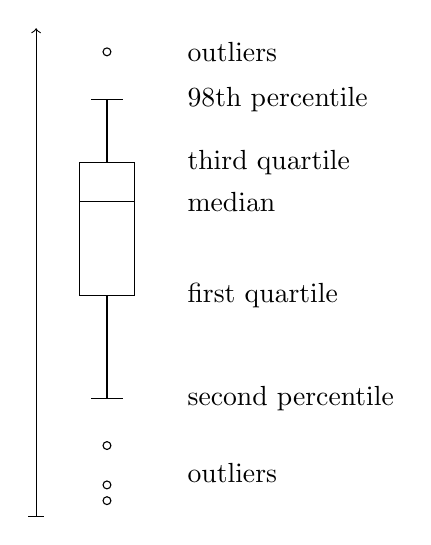
\begin{tikzpicture}[]

\def \xmid{0.9cm}
\def \xtext{1.8cm}
\def \boxwidth{0.7cm}
\def \whiskerwidth{0.4cm}

\def \youtlierbelowa{0.2cm}
\def \youtlierbelowb{0.4cm}
\def \youtlierbelowc{0.9cm}
\def \youtlierabove{5.9cm}

\def \ysec{1.5cm} % 2nd percentile
\def \yfir{2.8cm} % 1st quartile
\def \ymed{4.0cm} % median
\def \ythi{4.5cm} % 3rd quartile
\def \ynin{5.3cm} % 98th percentile

% y axis
\draw[->] (0cm , 0cm) -- (0cm, 6.2cm);
\draw[-] (-0.1cm, 0cm) -- (0.1cm, 0cm);

% hor lines from bottom to top
\draw[-] (\xmid - \whiskerwidth/2, \ysec) -- (\xmid + \whiskerwidth/2, \ysec);
\draw[-] (\xmid - \boxwidth    /2, \yfir) -- (\xmid + \boxwidth    /2, \yfir);
\draw[-] (\xmid - \boxwidth    /2, \ymed) -- (\xmid + \boxwidth    /2, \ymed);
\draw[-] (\xmid - \boxwidth    /2, \ythi) -- (\xmid + \boxwidth    /2, \ythi);
\draw[-] (\xmid - \whiskerwidth/2, \ynin) -- (\xmid + \whiskerwidth/2, \ynin);

% vert lines from bottom to top and left to right
\draw[-] (\xmid                  , \ysec) -- (\xmid              , \yfir);
\draw[-] (\xmid - \boxwidth    /2, \yfir) -- (\xmid - \boxwidth/2, \ythi);
\draw[-] (\xmid + \boxwidth    /2, \yfir) -- (\xmid + \boxwidth/2, \ythi);
\draw[-] (\xmid                  , \ythi) -- (\xmid              , \ynin);

% outliers from bottom to top
\node[draw, circle, inner sep=0pt, minimum size=0.1cm] at (\xmid, \youtlierbelowa) {};
\node[draw, circle, inner sep=0pt, minimum size=0.1cm] at (\xmid, \youtlierbelowb) {};
\node[draw, circle, inner sep=0pt, minimum size=0.1cm] at (\xmid, \youtlierbelowc) {};
\node[draw, circle, inner sep=0pt, minimum size=0.1cm] at (\xmid, \youtlierabove)  {};

% text from bottom to top
\node[draw=none, anchor=west] at (\xtext, \youtlierbelowa/2 + \youtlierbelowc/2) {outliers};
\node[draw=none, anchor=west] at (\xtext, \ysec)          {second percentile};
\node[draw=none, anchor=west] at (\xtext, \yfir)          {first quartile};
\node[draw=none, anchor=west] at (\xtext, \ymed)          {median};
\node[draw=none, anchor=west] at (\xtext, \ythi)          {third quartile};
\node[draw=none, anchor=west] at (\xtext, \ynin)          {98th percentile};
\node[draw=none, anchor=west] at (\xtext, \youtlierabove) {outliers};

\end{tikzpicture}

	\caption{Box plot}
	\label{fig:box-plot}
\end{figure}
The $p$th \emph{percentile} is the smallest value such that $p$ percent of all data points are less than or equal to that value.
The 50th percentile is also called the \emph{median}.
\emph{Quartiles} are multiples of the 25th percentile.
Inside the box of a box plot, half of all data points are located.
96\% of all values lie between the whiskers.
For a given function each process adds one data point to the distribution from which the box plot is derived.
Possible values for display are the accumulated exclusive time, average exclusive time, accumulated inclusive time, invocation count, performance counters and many others.
Accumulation and averaging is done over individual function calls.
Each function, function group or call stack configuration, depending on what is desired, is depicted as one box plot.
Imagine a traditional profile where bars are replaced with box plots to illustrate variation between processes.
Via mouse hovering, users can find out which processes lie in specific parts of the box plot.
Figure~\ref{fig:box-plot-profile-mockup} shows what this could look like.
Most performance analysis tools rely on minimum, average, maximum and some form of deviation for display.
These values strongly depend on outliers and may, thus, mislead.
Percentiles are robust to outliers, more intuitive and lead to a better understanding of a distribution.
Conclusions like ``50\% of all processes spend one to two seconds in \texttt{MPI\_Recv}.'' are impossible to draw from accumulated/selected values like minimum, average, maximum and deviation.
Another drawback is that deviation is indifferent to whether values lie above or below average.
Using percentiles, tendencies in variation can be displayed more clearly.
The downside is that obtaining percentiles is more costly in terms of computation and space.
\begin{figure}[tb]
	% traces/cosmo-specs-orig-100p-load-unbalanced
	\centering
	\includegraphics[width=12.6cm]{box-plot-profile-mockup} % 13.0cm / 667px * 648px = 12.6cm
	\caption{Excerpt of a box plot based-profile for a COSMO-SPECS run on 100 processes. The tooltip shows that process 50 and 63 to 87 are between the median and third quartile.}
	\label{fig:box-plot-profile-mockup}
\end{figure}

To ease access to the wealth of information contained in profiles, few well-defined starting points should be provided.
Not all scenarios where inclusive time, exclusive time and invocation count can be displayed make sense intuitively.
A call tree should, first and foremost, provide inclusive timing.
One can then repeatedly unfold functions where much inclusive time is spent, to locate points of interest.
If desired, the user can view additional information like exclusive time, invocation count and other performance metrics.
To find out where the most time in a program run is spent, one should first look at the accumulated exclusive time displayed per function group.
These groups can then be unfolded, e.g. by double-clicking, to inspect in which functions exactly the time is spent.
To find candidates for inlining, it makes sense to display a flat list of functions with their respective invocation count, perhaps in conjunction with average and/or accumulated exclusive time.
Other combinations of exclusive time, inclusive time, invocation count over functions, function groups or the call tree should only be supplied if the user desires.

Furthermore, it should be easy to find out which functions call a specific function, and which functions are called by it.
This enables users to quickly investigate where inclusive time is spent further down the stack or unwind a function into multiple entries to inspect timing and other metrics distinguished by calling location.

Emphasis should be put on avoiding to provide confusing or useless information.
Therefore, sensible sorting order defaults should be in place.
Additional orders help users obtain interesting information more quickly.
In general, the larger the accumulated exclusive time of a function, the more important it is.
Repeatedly calling a function using the same arguments, modulo external influences and global state, mostly yields the same execution time.
Therefore, large variations in accumulated exclusive time of a function between processes, especially when called via the same call path, hints at load imbalance.
A sorting order based on both accumulated exclusive time and its variation should, thus, be provided.
Another example for a helpful auxiliary order is sorting functions by invocation count paired with accumulated exclusive time.
This helps users find candidates for inlining.

In addition to these central features, there are lots of smaller ones that are to be realised.
Mind that smaller does not imply easier or quicker to implement.
Much of what follows is part of that extra mile which makes software good.
\begin{itemize}
	\item Users should be able to quickly search and filter for functions, processes and performance metrics everywhere.
		Searching for specific information in a given view can be tedious.
		For example, a simple search dialog (Ctrl+F) which highlights the searched word already helps.\vspace{-0.5ex}
	\item Proper undo and redo support is imperative.
		Neither HPCToolkit nor MAP have it.
		Users want to quickly go back and forth during an investigation and not having to remember the steps they take in order to do that.\vspace{-0.5ex}
	\item The user interface should be persistent.
		It ought to memorise the choices a user makes while navigating through different views, selecting functions, changing sort orders, moving up and down the stack.
		A view should be restored to its last state when being opened again.
		This includes storing an analysis session and restoring it once the same program is profiled again, or a previous profile is viewed.
		In general, the user interface should never present something unexpected or unintuitive.\vspace{-0.5ex}
	\item The user should be able to choose from viewing time in CPU cycles, seconds and percentages.\vspace{-0.5ex}
	\item Functions should automatically be grouped.
		Programs have hundreds and thousands of functions.
		Providing function groups improves overview and readability.
		VampirTrace~\cite{vampirtrace} provides very few default function groups.
		The successor Score-P and its file format OTF~2 do not support the concept of function groups.
		One has to improvise function groups using auxiliary information about programming paradigms and parallelism-specific properties, as is done in Vampir.
		These groups have to be generated automatically.
		Libraries, source files, \cpp~classes are likely candidates.
		Membership can be identified via string matching.\vspace{-0.5ex}
	\item Functions should be easy to regroup.
		Automatically generating a grouping that is 100\% correct and suits the users needs is hard if not impossible.
		Therefore, enabling easy and quick regrouping is key.
		One has to take extra care when functions are part of multiple groups, because it makes comparing values and applying percentages more difficult.
		A straightforward remedy is to only show mutually exclusive function groups.\vspace{-0.5ex}
	\item Cycle detection should be implemented.
		In recursive programs, straightforward calculation of inclusive timing, i.e. subtracting start from end time, leads to unintuitive results.
		For example, if $A$ takes 5 seconds of which 3 are used in a sub-call to $A$, then $A$ did not spend 8 seconds but 5.
		The inclusive time of a single function can, thus, exceed the execution time of the program.
		By using \emph{cycle detection}, the inclusive time of a function is only considered if this function is not already present on a lower stack level.
		This feature has been overlooked during Vampir development, and will be part of the next release.
\end{itemize}
Weaving these loosely organised threads together into a coherent tool potentially yields the best parallel profiler available.

This chapter demonstrates the effectiveness of the introduced techniques for two visualisations.
First, an existing one is improved.
Second, a novel profile viewer is proposed.
Its main contributions are greatly enhanced support for parallel programming and improved usability.

%%%%%%%%%%%%%%%%%%%%%%%%%%%%%%%%%%%%%%%%%%%%%%%%%%%%%%%%%%%%%%%%%%%%%%%%%%%%%%
\chapter{Conclusion \& Future Work}
\label{sec:conclusion}
This work introduces methods to cluster similar processes in sub-quadratic time.
For this purpose, it presents two measures.
One for detecting structural similarity between processes, and one to discern inlining and spawned threads from other differences.
Their effectiveness and efficiency to aid performance analysis is demonstrated using 15 different applications with up to 65,000 processes.
Due to their interesting characteristics, two of these applications are investigated in greater detail.
The improvement of an existing visualisation and introduction of a promising, novel profile viewer exhibit the aptitude of the methods to assist performance visualisation.

The contributions of this thesis advance comparative performance analysis and visualisation.
The introduced profile viewer improves over current ones, especially in support for parallel programming and usability.
Most notably, it visualises variations in performance measures, like timing and hardware performance counters, between processes using box plots.
With this, trends and outliers are easily spotted.

One of the investigated applications shows that the clustering approach is less effective for programs that exhibit irregular function call patterns.
This can be detected and steps to alleviate the situation are proposed.

Three categories of future directions of this work can be identified.
On the theoretical side, removing the requirement of van der Merwe's algorithm to retain duplicate attributes in the concept lattice would yield an appreciable speedup.
For that, a modification of the algorithm is to be devised.
To make the approach practical for every application, a method to reduce the lattice node count to arbitrary levels is needed.
It must retain meaningful and interesting information and yield intuitive program run lattices.
This reduction would also enable visualisation of the lattice itself.
This in turn, annotated with information about used APIs and parallel programming paradigms, can yield valuable insight into a program's structure.

A second direction is to advance the implementation.
To make it production-ready, the clustering should be parallelised, fall-backs must be implemented, and general optimisation is to be applied.

The third and last direction is to further software performance visualisation.
The proposed profile viewer has the potential to be the best in the field and is, therefore, to be implemented as a standalone tool or as a component of an existing visualisation tool, such as Vampir.
Leveraging the introduced techniques, novel visualisations to aid developers in understanding their programs and uncovering performance problems should be devised.

%%%%%%%%%%%%%%%%%%%%%%%%%%%%%%%%%%%%%%%%%%%%%%%%%%%%%%%%%%%%%%%%%%%%%%%%%%%%%%
\end{document}
